\chapter{High Voltage}
\label{ch:sp-hv}
%%%%%%%%%%%%%%%%%%%%%%%%%%%%%%%%%%%%%%%%%%%%%%%%%%%%%%%%%%%%%%%%%%%%
\section{High Voltage System Overview}
\label{sec:fdsp-hv-ov}

%%%%%%%%%%%%%%%%%%%%%%%%%%%%
\subsection{Introduction}
\label{sec:fdsp-hv-intro}

A \dword{lartpc} requires an equipotential cathode plane at \dword{hv} and a precisely regulated interior \efield{} to drive 
electrons from particle interactions to sensor planes.  In the case of the DUNE \dlong{sp} technology, 
this requires vertical cathode planes, called the \dword{cpa}, held at \dword{hv}; vertical anode planes, called \dwords{apa}, described in Chapter~\ref{sec:fdsp-apa-intro}; and formed sets of conductors at graded voltages surrounding the
 the central drift volume, collectively called the \dlong{fc}. The \dword{fc} consists of portions on the top and bottom  
of the drift volume (called the \dword{topfc} and \dword{botfc}, respectively), and along the sides, called \dwords{ewfc}.


The SP \dword{tpc} construction is shown in Figure~\ref{fig:dune_sp_fd}.
%A DUNE \dword{spmod} is made up of 4 drif, plus two complete  \dword{ewfc} planes, with 
The  drift fields transport the ionization electrons 
%in the direction \dword{cpa} $\Rightarrow$ \dword{apa}. 
towards the \dwords{apa} at sides and center.
One should note that the \dword{hv} systems for the \single and \dual TPC concepts share components with similar designs. These include the \dwords{fc} profiles and supporting FRP beams as well as the voltage divider boards. More details can be found in  Chapter 4.


\begin{dunefigure}[One unit of the \dword{spmod}]% showing \dwords{cpa} and \dwords{apa}]
{fig:dune_sp_fd}
{%Interior of a \dword{spmod}. The \dwords{cpa} occupy the second and fourth positions, between the three \dwords{apa}.  \Dwords{topfc} and \dwords{botfc} field cages are shown in blue (Image: CAD model).
A schematic of a \dword{spmod} showing the three \dword{apa} arrays (at the far left and right and in the center, spanning the entire \dword{detmodule} length) and the two \dword{cpa} arrays, occupying the intermediate second and fourth positions. The top and bottom \dword{fc} modules are shown in blue; the \dwords{ewfc} are not shown. 
On the right, the front top and bottom \dword{fc} modules are shown folded up against the \dword{cpa} panels to which they connect, as they are positioned for shipping and insertion into the cryostat.  The \dwords{cpa}, \dwords{apa} and \dwords{fc} together define the four drift volumes of the \dword{spmod}.}
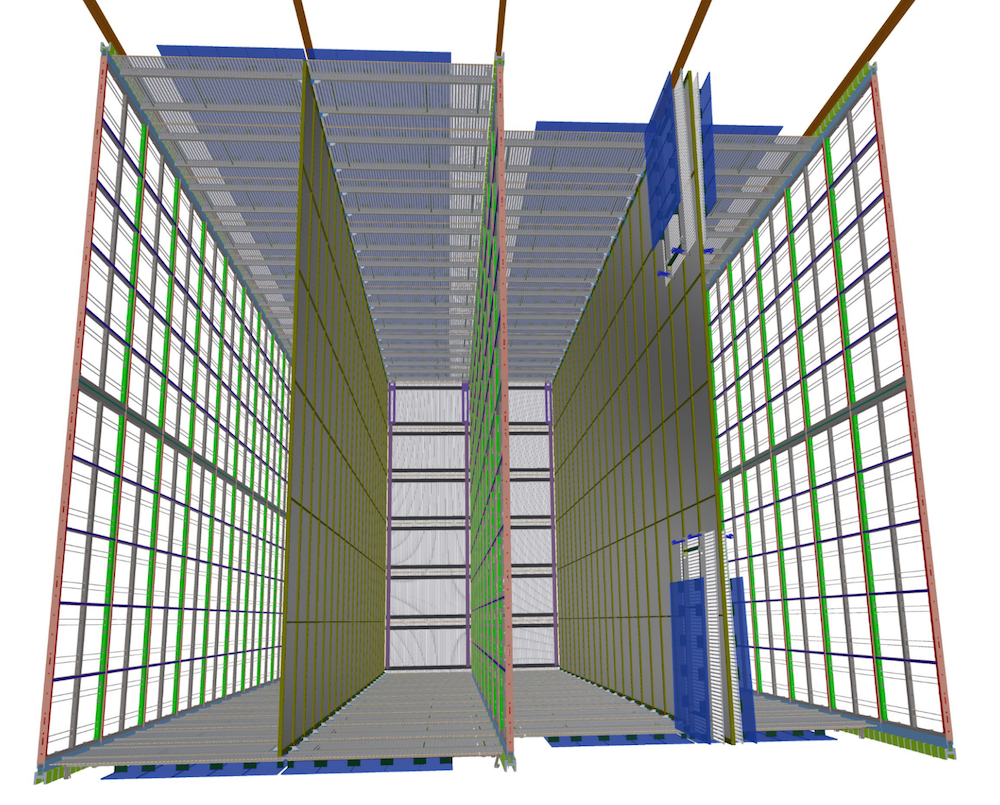
\includegraphics[width=0.8\textwidth]{dune_sp_fd}
\end{dunefigure}

The \dword{hv} consortium provides systems that operate at the full range of voltages, %all voltages, from the highest 
maximum to ground, inside the \dword{tpc} volume. As a result, its systems constitute a large fraction of the total internal structures of the \dword{tpc} itself, the principal exception being the \dwords{apa} and the \dword{pds}. In addition, the \dword{hv} system largely bounds the useful fiducial volume of the experiment, and thus plays a key role in determining the event rate for all DUNE physics processes. Mechanical and structural concerns are integrated with electrical design to meet the requirements. 

%\subsection{Design Considerations}

Two possible anode-cathode plane configurations exist for the fixed DUNE maximum electron drift length: cathode planes facing cryostat wall (C-A-C-A-C) or anode planes facing the cryostatic wall (A-C-A-C-A).  The latter configuration keeps most of the cathode plane surfaces far away from the grounded cryostat walls, reducing electrostatic breakdown risks and decreasing the total energy stored in the electric field to \SI{800}{J}.

In this configuration, energy is mostly stored in the high \efield{} region between the field cage and the nearby grounded conductors.  In an unexpected \dword{hv} breakdown, the entire \SI{400}{J} associated with one cathode could be released into a small volume of material, possibly causing physical damage.
%As an example, if this energy is converted to heat, it is sufficient to melt about 6\,mm$^3$ of stainless steel. 
It is difficult to predict the distribution of energy along a discharge path. A conservative approach treats this energy as a risk to the TPC and the cryostat membrane.  
%Given the size of the cryostat and the total TPC volume required, it is difficult to reduce this energy much further.  
Mitigating this risk entails slowing down the energy release as much as possible to minimize the potential damage by subdividing the \dword{fc} into electrically isolated modules, and constructing the cathode with highly resistive material.

Previous large \lartpc{}s (ICARUS, \microboone) have used continuous stainless steel tubes as electrodes. 
%There are disadvantages to scale this design to multi-kiloton  LArTPCs such as the DUNE Far Detector: 
Electrically, linking such electrodes to span more than \SI{100}{\m} in total length increases the stored energy each electrode has, and increases the risk of damaging the field cage components in a HV discharge. 
%Moreover, mechanically, such field cages cannot be built as completely independent modules and therefore require labor intensive steps to interconnect the electrodes, many at great heights inside the cryostat; 

Having the \dword{fc} divided into mechanically and electrically independent modules eases the construction and assembly of the \dword{fc}, and also greatly restricts the extent of drift field distortion caused by a resistor failure on the divider chain of a \dword{fc} module.

If the cathode is made of metal, a \dword{hv} discharge can cause the electrical potential of the entire cathode surface to swing from its nominal bias (e.g., \SI{-180}{kV}) to \SI{0}{V} in nanoseconds. This would induce a large current into the analog \dword{fe} amplifiers connected to the sensing wires on the \dwords{apa} (mostly to the first induction wire plane channels). Internal study (docdb 1320) has shown that this surge of current would overwhelm the internal ESD protection in the \dword{fe} ASICs.  To reduce this induced current, we chose to construct the cathode out of material with high resistivity.  Figure~\ref{fig:cpa-frame-discharge} shows the release of stored energy in time and the voltage distribution of a section of the cathode at one moment in time.  To minimize the induced current to the amplifiers, the surface resistivity should be raised until the ionization current from the TPC starts to cause significant voltage drop along the cathode.  In the DUNE FD the current is dominated by $^{39}$Ar decay, and we can tolerate surface resistivity well above \SI{1}{\giga\ohm/sq}. 


\begin{dunefigure}[Simulated \dword{cpa} discharge event]
{fig:cpa-frame-discharge}
{Bottom: Simulated \dword{cpa} Discharge event on a highly resistive cathode surface (1\,G$\Omega$/$\Box$), showing the voltage distribution on a section of the cathode (2.3\,m $\times$ 12\.m) 0.2\,ms after the discharge. Top: Time dependence of removal of stored energy.}
\centering
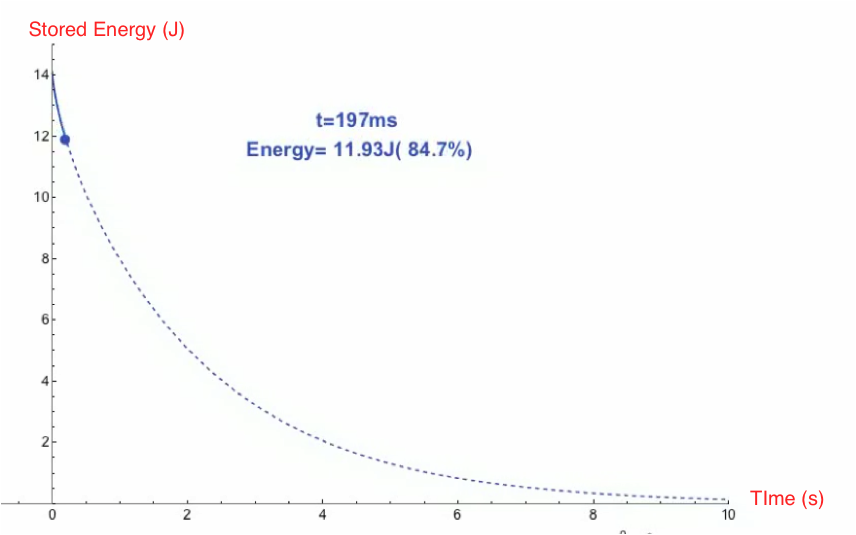
\includegraphics[width=0.6\textwidth,trim=2mm 2mm 2mm 2mm,clip]{A2r} \\ \vspace{30pt}    %update image with red labels, trim border
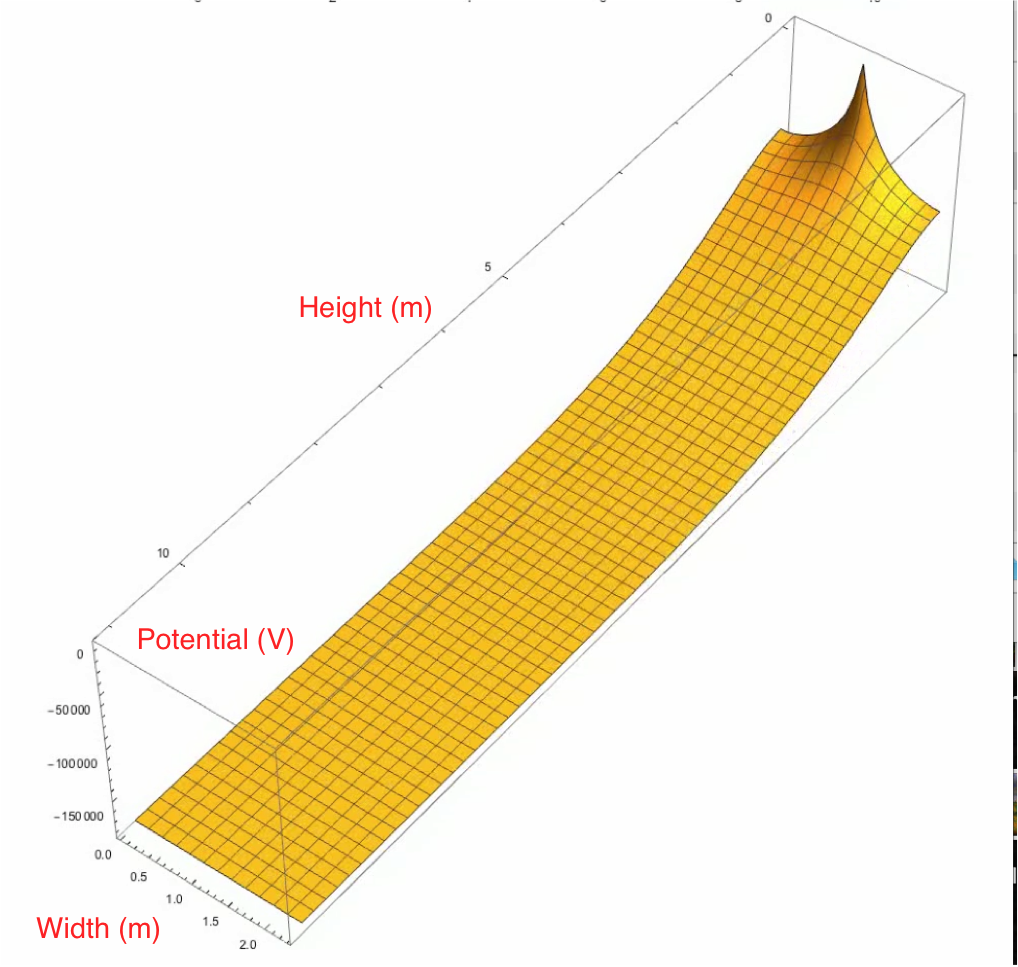
\includegraphics[width=0.5\textwidth,trim=2mm 2mm 2mm 2mm,clip]{A3r}
\end{dunefigure}

The SP \dword{hv} system may have modifications if problems are identified in the present design in \dword{pdsp}. Issues identified in earlier testing form the basis of an ongoing R\&D program.


%%%%%%%%%%%%%%%%%%%%%%%%%%%%
\subsection{Design Requirements}
\label{sec:fdsp-hv-des-consid}

%\fixme{Table of Requirements goes in this section.}
%\input{/files/generated/hv7fields-test}

The %\dword{tpc} 
\dword{hv} system is designed to meet the physics requirements of the DUNE experiment. These are both physical requirements (such as \efield{}s that allow robust event reconstruction) and operational (a system that avoids over-complication so as to maximize the time that the detector can collect neutrino events). An important collection of the requirements affecting \dword{hv} is shown in 
Table~\ref{tab:hvphysicsreqs}.
%\fixme{the most important requirements? Could there be multiple important collections of them? Also, the way some are worded they are impossible to verify (maximize, adequate...RKP: Language here was chosen carefully.}

\begin{dunetable}
[HV system requirements]
{p{0.05\textwidth}p{0.2\textwidth}p{0.35\textwidth}p{0.15\textwidth}p{0.15\textwidth}}
{tab:hvphysicsreqs}
{\dword{hv} system requirements}   
No. & Requirement & Physics Requirement Driver & Requirement & Goal \\ \toprowrule
1 & Establish uniform minimum \efield{} in \dword{tpc} drift volume. & Limit recombination, diffusion, and space charge impacts $e$, $\mu$, $p$ particle ID.  Establish constant drift velocity and adequate \dword{s/n} on induction planes for tracking. & >\SI{250}{V/cm} & \spmaxfield \\ \colhline
 2 & Do not exceed maximum \efield{} in \dword{lar} volume. %; subsystems that have been validated under working conditions in pure \lar may exceed cited limit. 
 & Avoid damage to detector to enable data collection over long periods. & \SI{30}{kV/cm} & \dword{alara} \\  \colhline
3 & Minimize power supply ripple & Keep readout electronics free from external noise, which confuses event reconstruction.  & 0.9~mV & 0.9~mV\\ \colhline
4 &  Maximize power supply stability. & Maintain ability to reconstruct data taken over long period.  Maintain high operational uptime to maximize experimental statistics. \\ \colhline
5 & Provide adequate resistivity to create acceptable decay constant for discharge of the cathode surface and \dword{fc}.  & Avoid discharge damage to \dword{detmodule} or electronics to enable data collection over long periods. %Value is set to allow extraction of stored energy over periods of seconds. Maintain high operational uptime to maximize experimental statistics.  
& \SI{1}{\mega\ohm}/sq & \SI{1}{\giga\ohm}/sq \\ \colhline
6 & Provide redundancy in all \dword{hv} connections. & Avoid single point failures in \dword{detmodule} that interrupt data collection. & Two-fold & Four-fold \\ 
\end{dunetable}
%\fixme{This should match the list of requirements that are eventually put into the DOORS system. Anne}

%%%%%%%%%%%%%%%%%%%%%%%%%%%%
\subsection{Scope}
\label{sec:fdsp-hv-scope}

%\fixme{Component Summary Table goes in this section}
%This section discusses 
The scope of the \dword{hv} system includes the selection and procurement of materials for, and the fabrication, testing, delivery and installation of systems to generate, distribute, and regulate the voltages that
create a stable and precise \efield{} within a DUNE \dword{spmod}. % the DUNE detector volume. 

The \dword{hv} system consists of components both exterior and interior to the cryostat. The voltage generated at the \dword{hv} power supplies passes through the cables, filters, and the \dword{hv} feedthrough into the cryostat. From the voltage delivery into the cryostat, it is further distributed by components that form part of the \dword{tpc} structure. 
These components are:
\begin{itemize}
\item \dword{hv} power supply;
\item \dword{cpa};
\item \Dword{topfc}, \dword{botfc}, and \dwords{gp};
\item \Dword{ewfc}.
\end{itemize}

%\fixme{Here I propose a figure that illustrates how these cpa and fc pieces relate to each other, could be based off of figure 11. Anne}
%\fixme{CPA was missing from the above items - I added it - SRM}

The \dword{tpc} has two \dwords{cpa} \textit{arrays}, that span the length and height of the \dword{spmod}, as shown in Figure~\ref{fig:dune_sp_fd}. Given the modular design, each array is assembled a set of 25 adjacent \dword{cpa} \textit{planes}, which in turn are constructed of smaller pieces.  Each plane is a set of two adjacent \textit{panels} (full height, half length, as measured along the \dword{detmodule} length). Each panel consists of three stacked \textit{units}, approximately \SI{4}{\m} high by \SI{1.2}{\meter} long. The units each consist of two half-height vertically stacked resistive panels enclosed within a FR4\footnote{NEMA grade designation for flame-retardant glass-reinforced epoxy laminate material, multiple vendors, National Electrical Manufacturers Association\texttrademark{},  \url{https://www.nema.org/pages/default.aspx}.} frame.

An  installation rail supports the panels from above through a single mechanical link.

%\fixme{Consortium contributed pgraph; see Anne's below}
The sides of the drift volumes on both sides of the \dword{cpa} plane are covered by the \dword{fc} and \dword{ewfc}  modules to define a uniform drift field of \spmaxfield{}, with a increasing potential over \SI{3.5}{m} from the \dword{hv} \dword{cpa} (\SI{-180}{kV}) to ground potential at the \dword{apa} sensor planes. The cathode bias is provided by an external \dword{hv} power supply through an \dword{hv} \fdth connecting to the \dword{cpa} plane inside the cryostat.
The \dword{fc} modules come in two distinct types: the top and bottom (\dword{fc}), which run the full length of the \dword{detmodule}, and the \dwords{ewfc}, %end walls (EW's), 
which complete the detector at either end. The modules of both systems are constructed from an array of extruded aluminum open profiles supported by FRP\footnote{Fiber-reinforced plastic, a composite material made of a polymer matrix reinforced with fibers, many vendors.} (fiber-reinforced plastic) structural beams. A resistive divider chain connects adjacent metal profiles to provide a linear voltage gradient between the cathode and anode planes.  The \dword{topfc} and \dword{botfc} modules are nominally  \SI{2.3}{\meter} wide by  \SI{3.5}{\meter} long. At the ends, the \dword{ewfc} modules are \SI{3.5}{\meter} wide by \SI{1.5}{\meter} in height.

Structurally, the frames of the cathode and field cages are made from materials with similar thermal expansion coefficients, minimizing issues of differential thermal expansion. The field cage frames support aluminum profiles but these are restrained at only one location and are allowed to float within the frame.
%Cold testing of a \dword{cpa}, with monitoring of its geometry and electrical resistance is documented in DocDB 2338. In addition, Docdb 1504 documents the testing at cryogenic temperatures of kapton/FR4 laminates and the shrinkage of the detector was examined in Docdb 6011.
%Each \dword{topfc} and \dword{botfc} module is nominally \SI{2.3}{\m} wide by  \SI{3.5}{\m} long (along the \dword{detmodule} length). 
The \dwords{ewfc} modules, each \SI{1.5}{\m} high by \SI{3.5}{\m} wide (along the drift volume dimension), stack eight units high to cover the \tpcheight{} height of the \dword{tpc}.  
Extensive tests have been performed of mechanical and electrical properties of materials used in the \dword{hv} system.  These are fully documented elsewhere\fixme{Add to bib: \textit{CPA Electrical Connections Cold Test}, DUNE DocDB 2338; \textit{CPA and FC Design}, DUNE DocDB 1504; \textit{Technical Review: Mechanical Specifications for \dword{pdsp} \dword{fc} test in \dword{35t} at \fnal}, DUNE DocDB 1601.
}

The \dwords{cpa} and \dwords{apa} support the \dword{topfc} and \dword{botfc} modules, whereas
%The \dword{topfc} and \dword{botfc} modules are supported by the \dwords{cpa} and \dwords{apa}. 
%The \dwords{ewfc} modules are \SI{1.5}{\meter} tall by \SI{3.5}{\meter} long. They are stacked eight units high to cover the \SI{12}{\meter} height of the \dword{tpc}.  
installation rails above the \dwords{apa} and \dwords{cpa} support the \dword{ewfc} modules. 
%are supported by the installation rails above  the \dwords{apa} and \dwords{cpa}, which are part of the \dword{dss}. 
A \dlong{gp} consisting of tiled, perforated stainless steel sheets % panels %is mounted on 
runs along the outside surface of each of the %top and bottom \dword{fc} modules 
\dword{topfc} and \dword{botfc}, with a \SI{20}{\centi\meter} clearance. 

%For ease of understanding the rather complex physical layout of the systems comprising the \dword{hv} and \efield{} hardware, 
Tables~\ref{tab:cpaparts} and~\ref{tab:fcparts} contain summaries of terminology and parts.

\begin{dunetable}
[\dword{hv} \dword{cpa} components]
{p{0.4\textwidth}p{0.12\textwidth}
p{0.12\textwidth}p{0.32\textwidth}}
{tab:cpaparts}
{\dword{hv} Cathode Plane Components} 
Component and Quantity &  Length (z) & Height (y) & Per \dword{spmod} \\ \toprowrule
\dword{cpa} Array (2 per \dword{spmod}) & \SI{58}{\meter} & \SI{12}{\meter} & 2  \\ \colhline
\dword{cpa} Plane (25 per \dword{cpa} Array)  & \SI{2.3}{\meter}  &\SI{12}{\meter} & 50  \\ \colhline
\dword{cpa} Panel (2 per \dword{cpa} Plane)  & \SI{1.2}{\meter}   & \SI{12}{\meter} & 100  \\ \colhline
\dword{cpa} Unit (3 per \dword{cpa} Panel)  & \SI{1.2}{\meter}  & \SI{4}{\meter} & 300 \\ \colhline
\dword{cpa} RP (2 per \dword{cpa} Unit)  & \SI{1.2}{\meter}  & \SI{2}{\meter} & 600 \\
\end{dunetable}


\begin{dunetable}
[\dword{hv} \dword{fc} components]
{p{0.37\textwidth}p{0.07\textwidth}p{0.07\textwidth}p{0.07\textwidth}p{0.07\textwidth}
p{0.1\textwidth}p{0.15\textwidth}}
{tab:fcparts}{\dword{hv} Field Cage Components}
Component & Count & Length (z) & Width (x) & Height (y) & Submodules & Grand Total \\ \toprowrule
\dword{fc} (Top/Bottom Field Cage) & 200 & 2.3 m & 3.5 m & - & 57 & 200 \\ \colhline
\dword{fc}-Profiles (per \dword{fc}) & 57 & 2.3 m & - & - & - & 11400 \\ \colhline
Ground Plane Modules (per \dword{fc}) & 5 & 2.3 m & 0.7 m & - & - & 1000 \\ \colhline
EW-Plane (Endwall Field Cage) & 2 & - & 14.4 m & 12 m & 4 & 2 \\ \colhline
EW (per EW-Plane) & 4 & - & 3.5 m & 12 m & 8 & 8 \\ \colhline
EW-Modules (per EW) & 8 & - & 3. m & 1.5 m & 57 & 64 \\ \colhline
EW-Profiles (per EW-Module) & 57 & - & - & 1.5 m & - & 3648 \\
\end{dunetable}
\clearpage
%%%%%%%%%%%%%%%%%%
\subsection{Design Safety}
\label{fdsp-hv-design-safety}

Safety is central to the design of the \dword{hv} system. In all phases including fabrication, installation, and operations, safety will be the highest priority. There will be documented assembly, testing, transport, and installation procedures. Particular attention was paid to these topics in the design of  
\dword{pdsp}  with explicit concern to a design that is identical to the \dword{spmod} design, the most critical of which are also noted in the preliminary \dword{hv} risk assessment, which is under development. %Commented for IDR -\fixme{ref properly. RKP: Requires reference policy, under discussion.}

The structural and electrical designs for the \dword{sp} \dword{hv} are based on designs that were vetted and validated in the \dword{pdsp} construction. Previously, Fermilab \dword{hv} tests implemented a full-voltage and full-scale \dword{hv} feedthrough, power supply, filtering, and monitoring system, along with the \dword{hv} connection cup and arm, after completing full safety reviews. These devices worked as designed and are essentially reproduced in both \dword{pdsp} and the \dword{spmod}. 

When operating the \dword{fc} at its full operating voltage there is a substantial amount of stored energy. The design of the \dword{cpa} is centered around storing charge  at the highest voltage on a resistive surfaces to limit the power dissipated during a power supply trip or other failure which unexpectedly drops the \dword{hv}. This design has been successfully tested at full voltage over \num{2}\,m$^2$ surfaces and at larger scale in \dword{pdsp}.  

Integral to the \dword{sp} \dword{fc} design, both in \dword{pdsp} and the \dword{spmod}, is the concept of pre-assembled modular panels of field-shaping conductors with individual voltage divider boards. The structural design and installation procedures used in \dword{pdsp} were selected to be compatible with use at the Far Detector site and were vetted by project engineers, engineering design review teams, and CERN's safety engineers. Any revisions to these designs based on lessons learned in \dword{pdsp}  installation and operations will be reviewed both within the Project and by Fermilab \dword{esh} personnel. The overall design is on solid footing. 

%%%%%%%%%%%%%%%%%%%%%%%%%%%%%%%%%%%%%%%%%%%%%%%%%%%%%%%%%%%%%%%%%%%%
\section{ProtoDUNE-SP High Voltage Experience}
%NOTE -- this is a work in progress... still needs to be refined...
%NOTE a nice number to quote somewhere in this section will be the uptime % during the beam run
\label{sec:fdsp-hv-protodune}
The protoDUNE-SP detector \cite{protoDUNSP-tdr} is a prototype for the single phase \lartpc \dword{dune} far detector.
Approximately 1/20th the size of a DUNE 10kt module, protoDUNE-SP contains one CPA array, which bisects the TPC, and two APA arrays arranged in an A-C-A configuration.
The CPA array is built up from three CPA planes with dimensions 2.3m $\times$ 6.0m and is positioned 360 cm away from each CPA array, matching the maximum drift distance of a DUNE module.
Six top FC units and six bottom FC units connect the horizontal edges of the CPA and APA arrays, and four endwalls connect the vertical edges.
Each endwall is comprised of four endwall modules.
A Heinzinger -300kV 0.5mA high voltage power supply delivers voltage to the cathode.
Two HV filters in series between the power supply and HV feedthrough filter out high frequency fluctuations upstream of the cathode.

\begin{dunefigure}[ProtoDUNE-SP TPC HV components]
{fig:protodune_sp_hv}
{One of the two drift volumes of the protoDUNE-SP detector. The FC modules are shown enclosing the drift volume between CPA array(middle) and APA array (right). The end wall FCs are oriented vertically while the top and bottom units are horizontal. The staggered printed circuit boards connecting the FC profiles are the voltage divider boards, which introduce a uniform resistance between neighboring electrodes.}
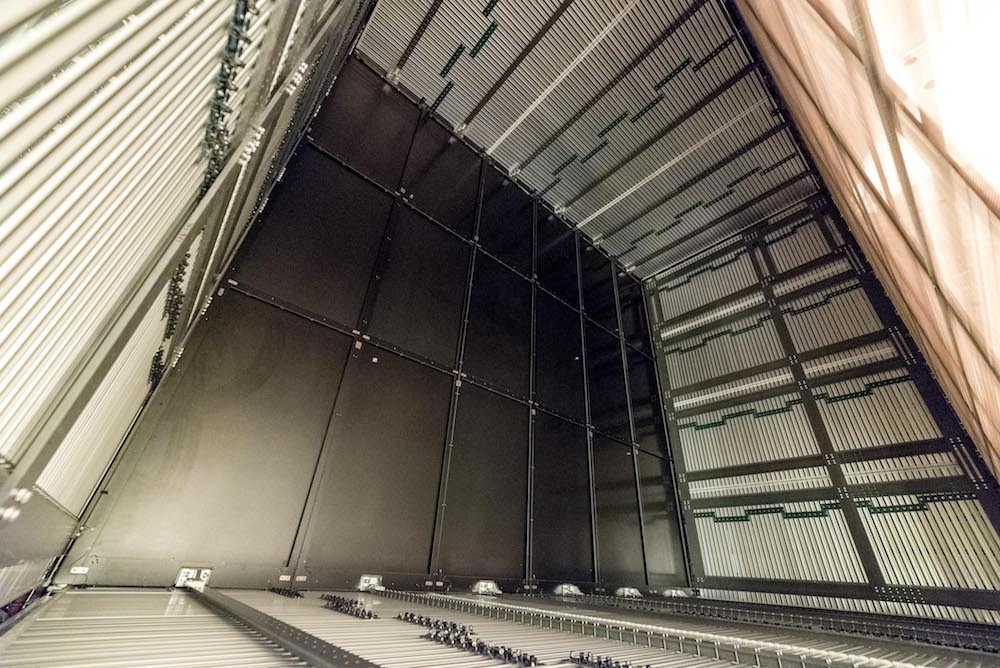
\includegraphics[width=0.8\textwidth]{protoDUNE-SP_TPCHV}
\end{dunefigure}

\subsection{Summary of Construction and Operation}
The \dword{tpc} \dword{hv} components underwent some level of preassembly off site.
Parts for the top and bottom field cage frames were acquired and test fit at Stony Brook University before being shipped to CERN for module assembly in a clean room about 5km away from the detector hall.
Fully assembled modules were transported on a flatbed to the detector hall for storage until installation.
Similarly, end wall frame parts were aqcuired and test fit at Louisiana State University before being sent to CERN.
In this case, the end wall frames were sent fully assembled, and the field shaping profiles were installed and voltage dividor boards mounted in the same CERN clean room facility.
CERN provided the field shaping profiles and, in the case of the top and bottom FC units, the ground planes, while Louisiana State University provided all voltage divider boards.
The \dword{cpa} material was sent to the detector hall from Argonne in preassembled resistive panels held in a G10 frame.

In the ProtoDUNE-SP cleanroom, the resistive panels were connected, mechanically and electrically, into a 3x2 grid to produce a cathode plane unit of a size corresponding to that of an \dword{apa}, as shown on the left in Figure~\ref{fig:cpas-in-cryostat}.
Two 3-panel-tall columns (one of which is pictured in Figure~\ref{fig:cpa_panel-complete}) were assembled horizontally and lifted to vertical to be connected while suspended.
Two top and two bottom FC modules were brought into the clean room, lifted to vertical and attached to the \dword{cpa}.
Once the load was transfered onto the \dword{cpa}, the top FCs were allowed to hang vertically below their support at the top of the CPA, and the bottom FCs were folded up and attached to their top FC counterparts.
The resulting CPA-FC assemblies were rolled onto the central bridge beam inside the cryostat.

Also in the ProtoDUNE-SP clean room, the end walls were built out of the preassembled panels (4 panels/end wall).
The beam plug was also installed onto the corresponding panel here before the beam right, upstream endwall was built.
An electric hoist was used to lift the top panel to a height where the next panel can be wheeled underneath and connected via FRP plates.
The hoist would then raise the pair and the procedure would continue in this way until the endwall was 4 panels tall.
The load of the end wall was then transfered to a trolley on a transport beam, which allowed the assembly to be pushed into the cryostat onto the appropriate bridge beam.

The TPC components of ProtoDUNE-SP were installed first for the beam right drift and then for the beam left.
The APAs and CPAs were locked into position along their respective bridge beams, and then the bridge beams were locked into their position along the drift direction.
Next, 2 end walls were moved and rotated into their upstream and downstream positions to bridge the gap between the vertical edges of the corresponding APA and CPA.
The end wall loads were transfered onto the APA and CPA bridge beams, which freed the intermediate bridge beam for top/bottom field cage deployment.
Two mechanical hoists were used to lower (raise) the bottom (top) field cages to bridge the gap between the horizontal edges of the APAs and CPAs.
Finally, the HV cup was connected on the downstream CPA, and the HV feedthrough was lowered through the cryostat penetration to make contact with the cup.

During the cool-down and \dword{lar} filling, a field cage termination power supply was used to supply -1kV to the cathode and monitor the current draw of the system.
As the system cooled from room temperature to \dword{lar} temperature, the resistance increased by $\sim$10\%.

TOADD:
\begin{itemize}
\item beam-run conditions/operations (``streamers'' exist, costs about 10 minutes per 4 hrs of operation)
\begin{itemize}
\item uptime \% during beam on periods (>90\%, needs to be calculated still)
\end{itemize}
\end{itemize}

\label{sec:fdsp-hv-protodune-summary}
%%%%%%%%%%%%%%%%%%%%%%%%%%%%

\subsection{Lessons from ProtoDUNE}
\label{sec:fdsp-hv-protodune-lessons}
The protoDUNE-SP HV experience was, in general, a very encouraging one.
An ability to operate the TPC with a drift field of 500 V/cm was demonstrated.
However, throughout the run the system did experience various instabilities, the source of which are in the process of being investigated further.
A more systematic study will be able to be made after the test beam run.

\subsubsection{Design}
\label{sec:fdsp-hv-protodune-lessons-design}
The general design of the DUNE HV system was validated by the success of protoDUNE-SP, although various opportunities for improvement were noted during its construction and operation:

\begin{itemize}
\item Adopting a ``pot-style'' filter design would prevent leaks from causing interventions for refilling.
\item Raising the cable insert to the HV feedthrough above the cold insulation space (if space allows). In the event the cable needs to be removed from the feedthrough, there is danger of moisture freezing on the walls and preventing good electrical contact. \item Toroid signals would be a welcomed addition to the feedthrough.
\item Increasing the distance between the ground planes and field shaping profiles and eliminating direct paths for potential surface currents could improve stability.
\end{itemize}

It is worth noting, the instrumented ground planes on the top and bottom field cages proved to be a valuable source of information during moments of instability.
Furthermore, having a dedicated data acquisition system to readout the signals from the ground plane monitoring system, beam plug current monitor, and power supply read back at a rate of 20 kHz upon a trigger, provided very useful information for diagnosing the high voltage behavior inside the TPC.
This system was not run continuously, but requires significant disk space to store the data it awuire

\subsubsection{Part Production and Handling}
\label{sec:fdsp-hv-protodune-lessons-assy}
The production and handling of HV components must be approached with sufficient care to avoid compromising the electrical components or introducing scratches and other sharp edges.
The aluminum field shaping profiles are particularly prone to acquiring scratches if they are not packaged and handled in such a way to avoid direct contact with other profiles and materials.
Kapton strips separated the profiles and the FRP of the FC frames as they were being inserted to avoid scratching and removal of the profile coating.
If scratches were found in the FRP beams, they were covered with epoxy to prevent fibers from escaping into the \dword{lar}.

QC tests were conducted on sub-modules and individual components at every step of the construction - part procurement, assembly, integration, and installation.
Individual components or assembled submodules that were shipped to another facility had their previously administered QC tests repeated to ensure nothing was compromised during transport. 
%Resistance between steps on the voltage divider boards were measured and verified to be within specification both after their production at LSU and after they were shipped to CERN.
%Once the voltage divider boards were mounted onto an assembled FC module, the resistance between adjacent profiles was measured to verify sound electrical connection 
\begin{itemize}
\item avoid sharp edges
\begin{itemize}
\item buckling of ground plane corners when being pressed
\end{itemize}
\end{itemize}


\subsubsection{Assembly and Installation}
\label{sec:fdsp-hv-protodune-lessons-assy}
\begin{itemize}
\item FC module assembly - 1.5 days/module with 2 workers
\item EW module assembly - 1.5 days/module with 2 workers
\item CPA plane - 2 days/plane with 4 workers
\item CPA plane + FC integration - 1 day/assembly with 4 workers
\item QC throughout the assembly and installation process invaluable (examples)
\item bowing of end wall when connecting panels and fix
\item misalignments when TPC is partially deployed
\end{itemize}

\subsubsection{Performance}
\label{sec:fdsp-hv-protodune-lessons-perf}
\begin{itemize}
\item Continuous operation at -180kV on the cathode
\item Fast discharges
\item "Streamers" (no impact on TPC signals observed, some evidence on PDS)
\end{itemize}

%%%%%%%%%%%%%%%%%%%%%%%%%%%%

\subsection{Suggestions for future R\&D}
\label{sec:fdsp-hv-protodune-RD}
From the ProtoDUNE-SP experience, a number of R\&D items have been proposed including:
\begin{itemize}
\item Evaluate the charge and discharge behavior of the UHMW PE caps on the end of the profiles compared to metallic capped profiles.  The goal is to check if the PE endcaps contribute to HV instability.
\item Compare the HV stability of 90 degree bent profiles with capped profiles at right angle.  The goal is to check if the bent profiles are more stable for HV performance than a capped design meeting at a right angle.
\item Evaluating resistive/metallic caps.  If the PE caps are shown to be problematic, find an alternative solution to maintain segmented field cage modules.
\item Study the surface charging behavior of the field cage insulation structures.  Evaluation of general insulator performance for LArTPCs including charge-up effects and geometry remains an outstanding task.  In this test, the goal is to find out if any geometrical feature or surface treatment can reduce HV instability.
\item Evaluation of higher resistivity Kapton films.  The goals is to check the feasibiligy of increasing the surface resistivity of the cathode plane up to 1~G$\Omega$/square.  The task includes verifying the lamination quality on FR4 sheet and production availability.
\item Full HVS discharge behavior study (Spice simulation).  While modelling other field cage designs and DUNE will take considerable effort, the possibility of understanding the source of instabilities or exposing any design weaknesses makes this a worthwhile endeavor.
\end{itemize}
\clearpage

%%%%%%%%%%%%%%%%%%%%%%%%%%%%%%%%%%%%%%%%%%%%%%%%%%%%%%%%%%%%%%%%%%%%

\section{HV System Design}
\label{sec:fdsp-hv-design}

%%%%%%%%%%%%%%%%%%%%%%%%%%%%
\subsection {High Voltage Power Supply and Feedthrough}

The \dword{hv} delivery system consists of
\begin{itemize}
\item two power supplies,
\item \dword{hv} cables,
\item filter resistors, and
\item \dword{hv} feedthroughs into the cryostat.
\end{itemize}

For \dword{hv} delivery, two power supplies are used to generate the voltage, one for each \dword{cpa} array. 
This separated setup more easily accommodates different running conditions and helps isolate any instabilities. %In addition, t
The cryostat design has two feedthrough ports for each \dword{cpa} array, one at each end of the cryostat. The spare, downstream port provides redundancy against any failure of the primary \dword{hv} delivery system. 
%In the event only one power supply is available, the system will be run by using a \dword{hv} splitter outside of the cryostat while another power supply is procured. 

Each \dword{cpa} connects to two drift volumes in parallel, presenting a net resistance of \SI{1.14}{\giga\ohm} to each supply. At the nominal \SI{180}{kV} cathode voltage, each power supply must provide \SI{0.16}{mA}.

The planned power supply model for the \dword{spmod} is similar to the power supply\footnote{Heinzinger, PNC HP200000 \dword{hv} power supply, Heinzinger\texttrademark{} Power Supplies, \url{http://www.heinzinger.com/}.} used on \dword{pdsp} %, with a maximum output voltage of \SI{200}{kV} and a maximum current draw of \SI{0.5}{mA}.  
An %additional 
option is an existing \SI{300}{kV}, \SI{0.5}{mA} model from the same vendor.
The \dword{hv} cables are commercially available models compatible with the selected power supplies. 

%The \dword{hv} cables will be either Dielectric Sciences model number 2134 capable of \SI{200}{kV} DC or 2236 capable of \SI{320}{kV} DC. 
%ielectrThe \dword{hv} cables are preferred to be Dielectric Sciences model number 2134 capable of \SI{200}{kV} DC.  A back up plan is to use model 2236 capable of \SI{320}{kV} DC. 

Filter resistors are placed in between the power supply and the feedthrough.  Along with the cables, these resistors reduce the discharge impact by partitioning the stored energy in the system.  The resistor-cable assembly also serves as a low-pass filter reducing 
the \SI{30}{kHz} voltage ripple on the output of the power supply.  With filtering, such supplies have been used successfully in other \lartpc experiments, such as \microboone and ICARUS.

Figure~\ref{fig:ps_filter_ft_schematic} provides a sample schematic of the \dword{hv} supply circuit.

\begin{dunefigure}[A schematic showing the \dword{hv} delivery system to the cryostat.]  %The two filters are placed such that one is near the power supply and one is near the feedthrough.
{fig:ps_filter_ft_schematic}
{Right:  A schematic showing the \dword{hv} delivery system to the cryostat (Credit:  SEL). %The two filters are places such that one is near the power supply and one is near the feedthrough. 
One of the two filters sits near the power supply; the other sits near the feedthrough. Left:   %An example 
A Heinzinger power supply (Credit: H.~Wang).}
%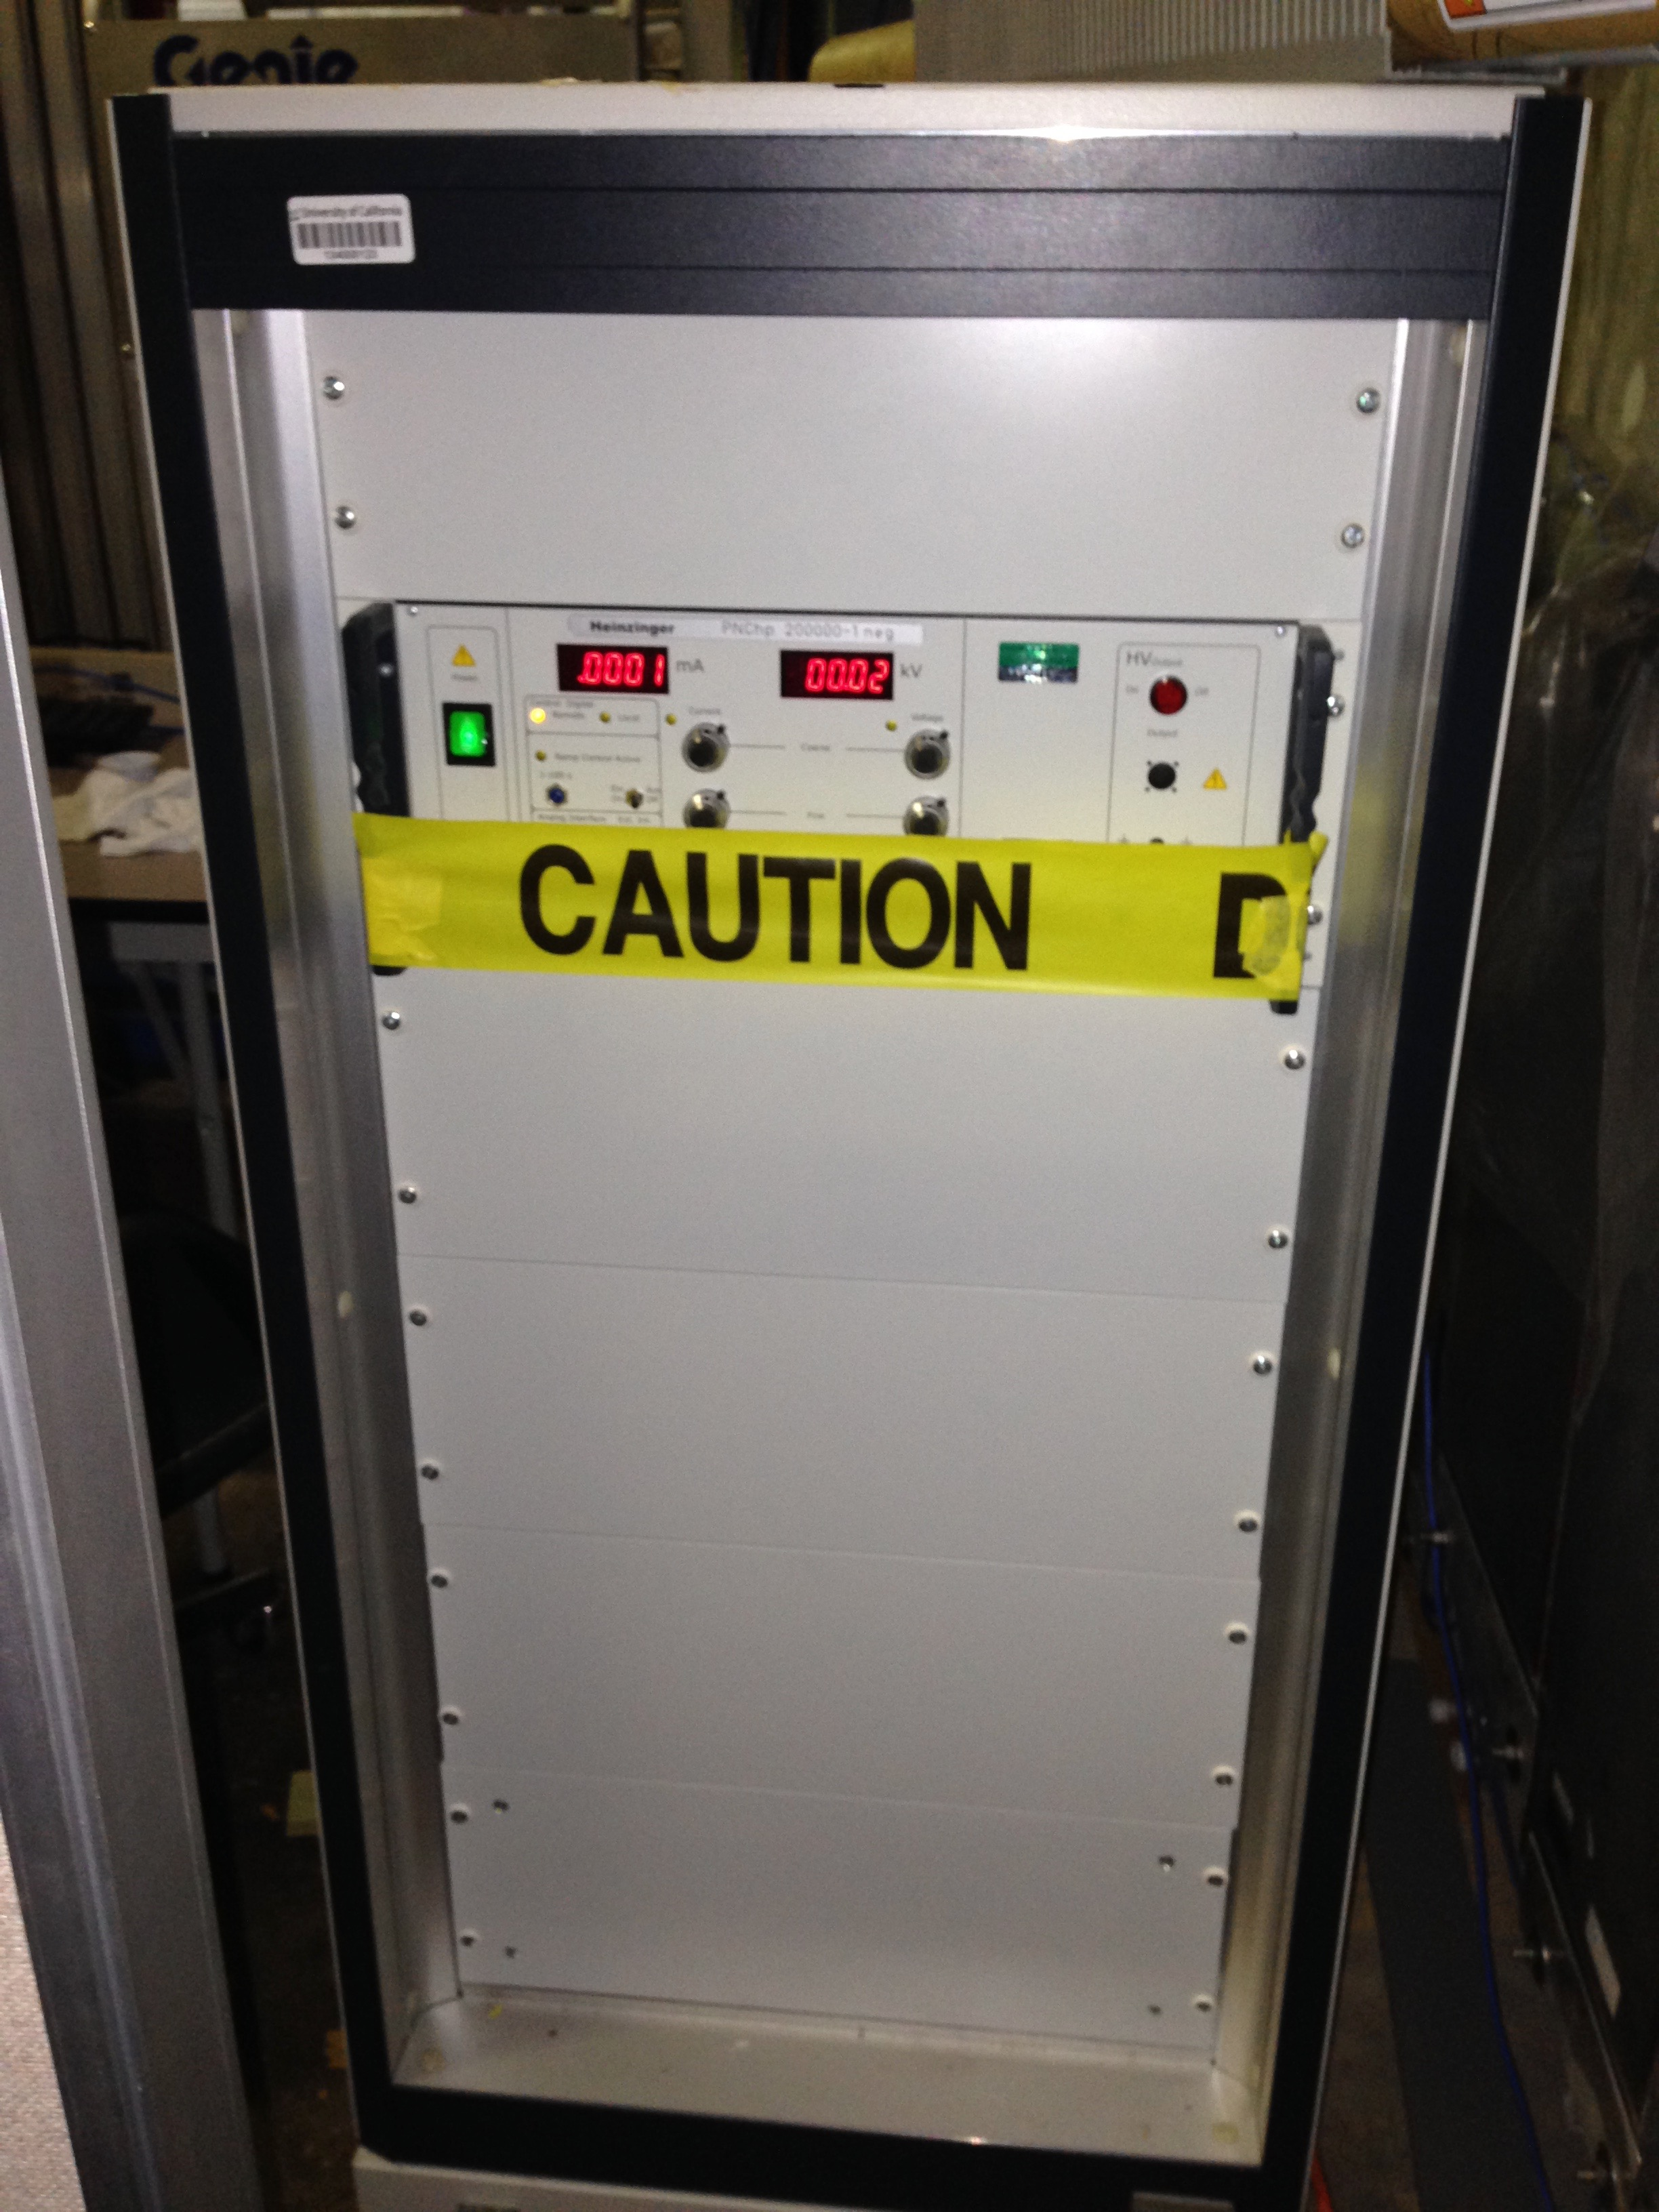
\includegraphics[width=0.2\textwidth]{heinzy}
%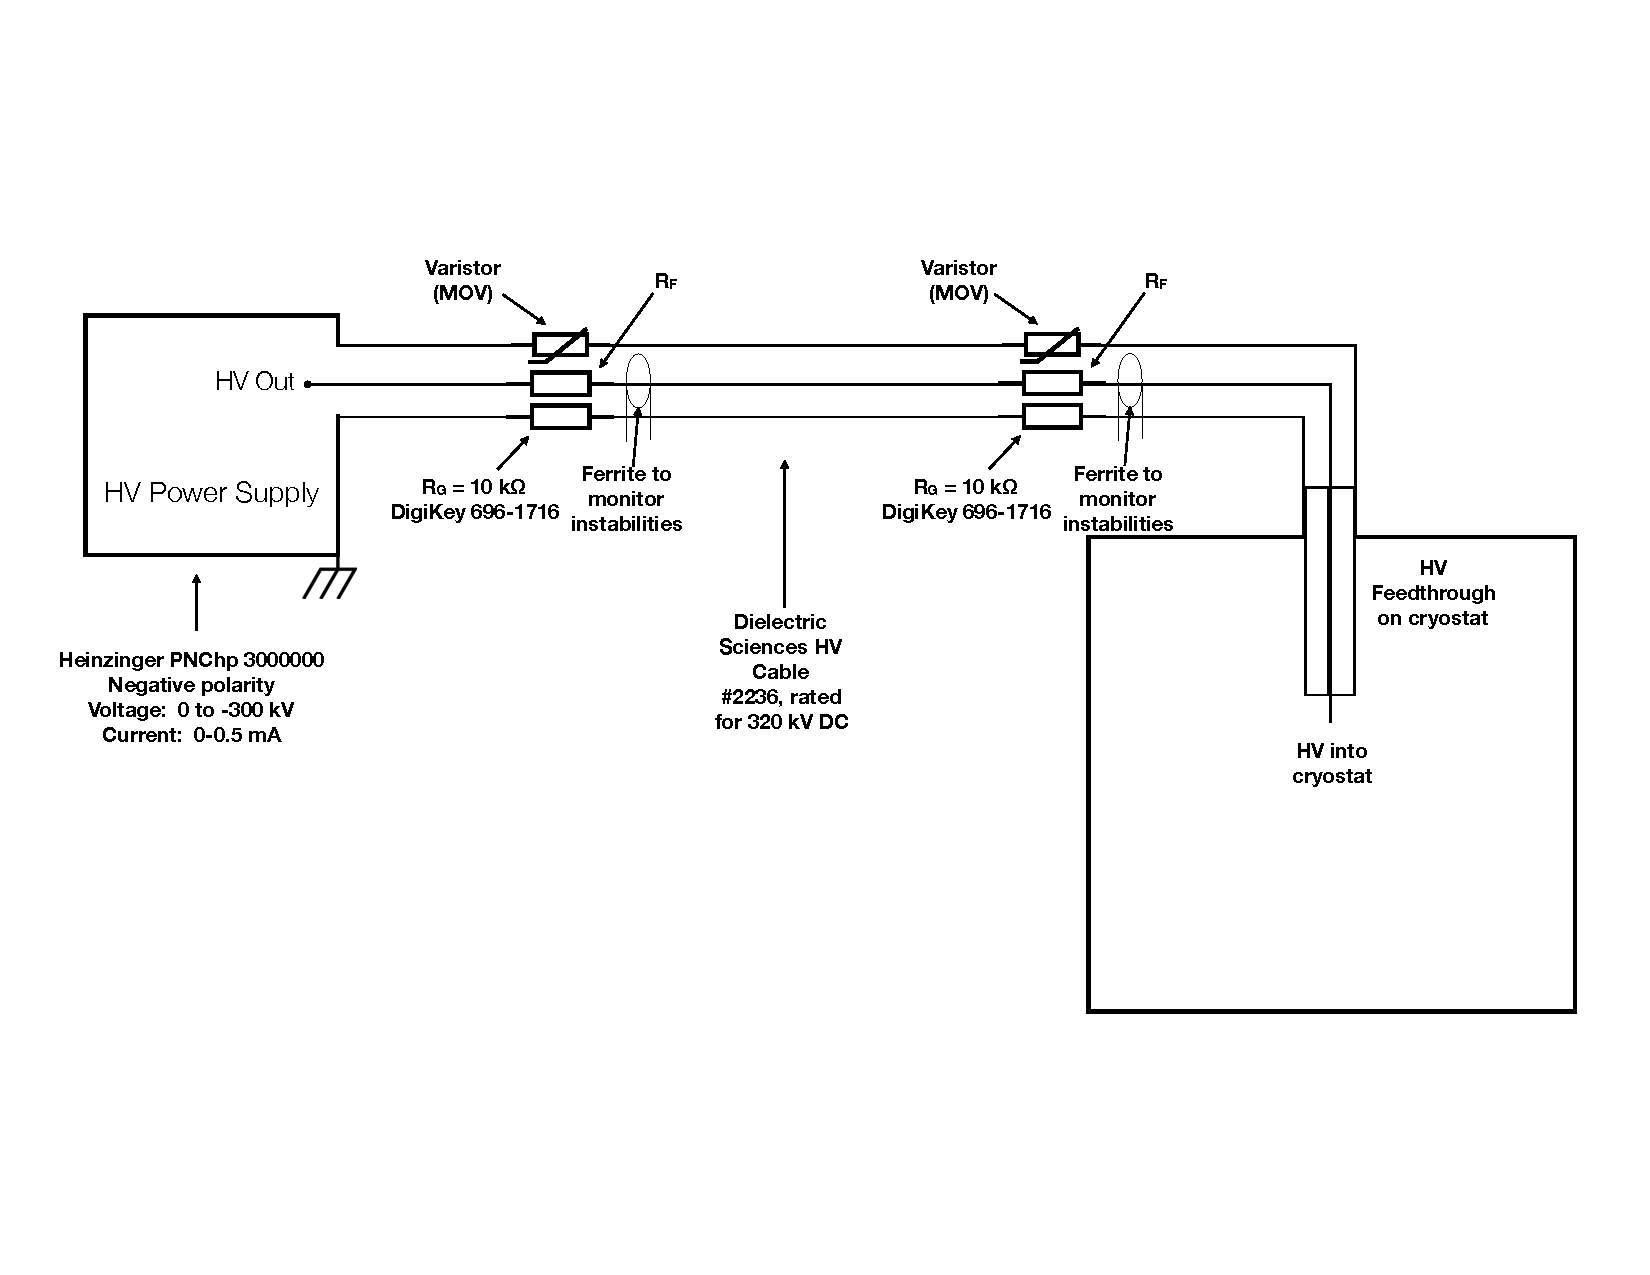
\includegraphics[width=0.7\textwidth]{ps_filter_ft_schematic}  %requested image edits by DeMuth
\begin{minipage}{6in}
  \centering
  $\vcenter{\hbox{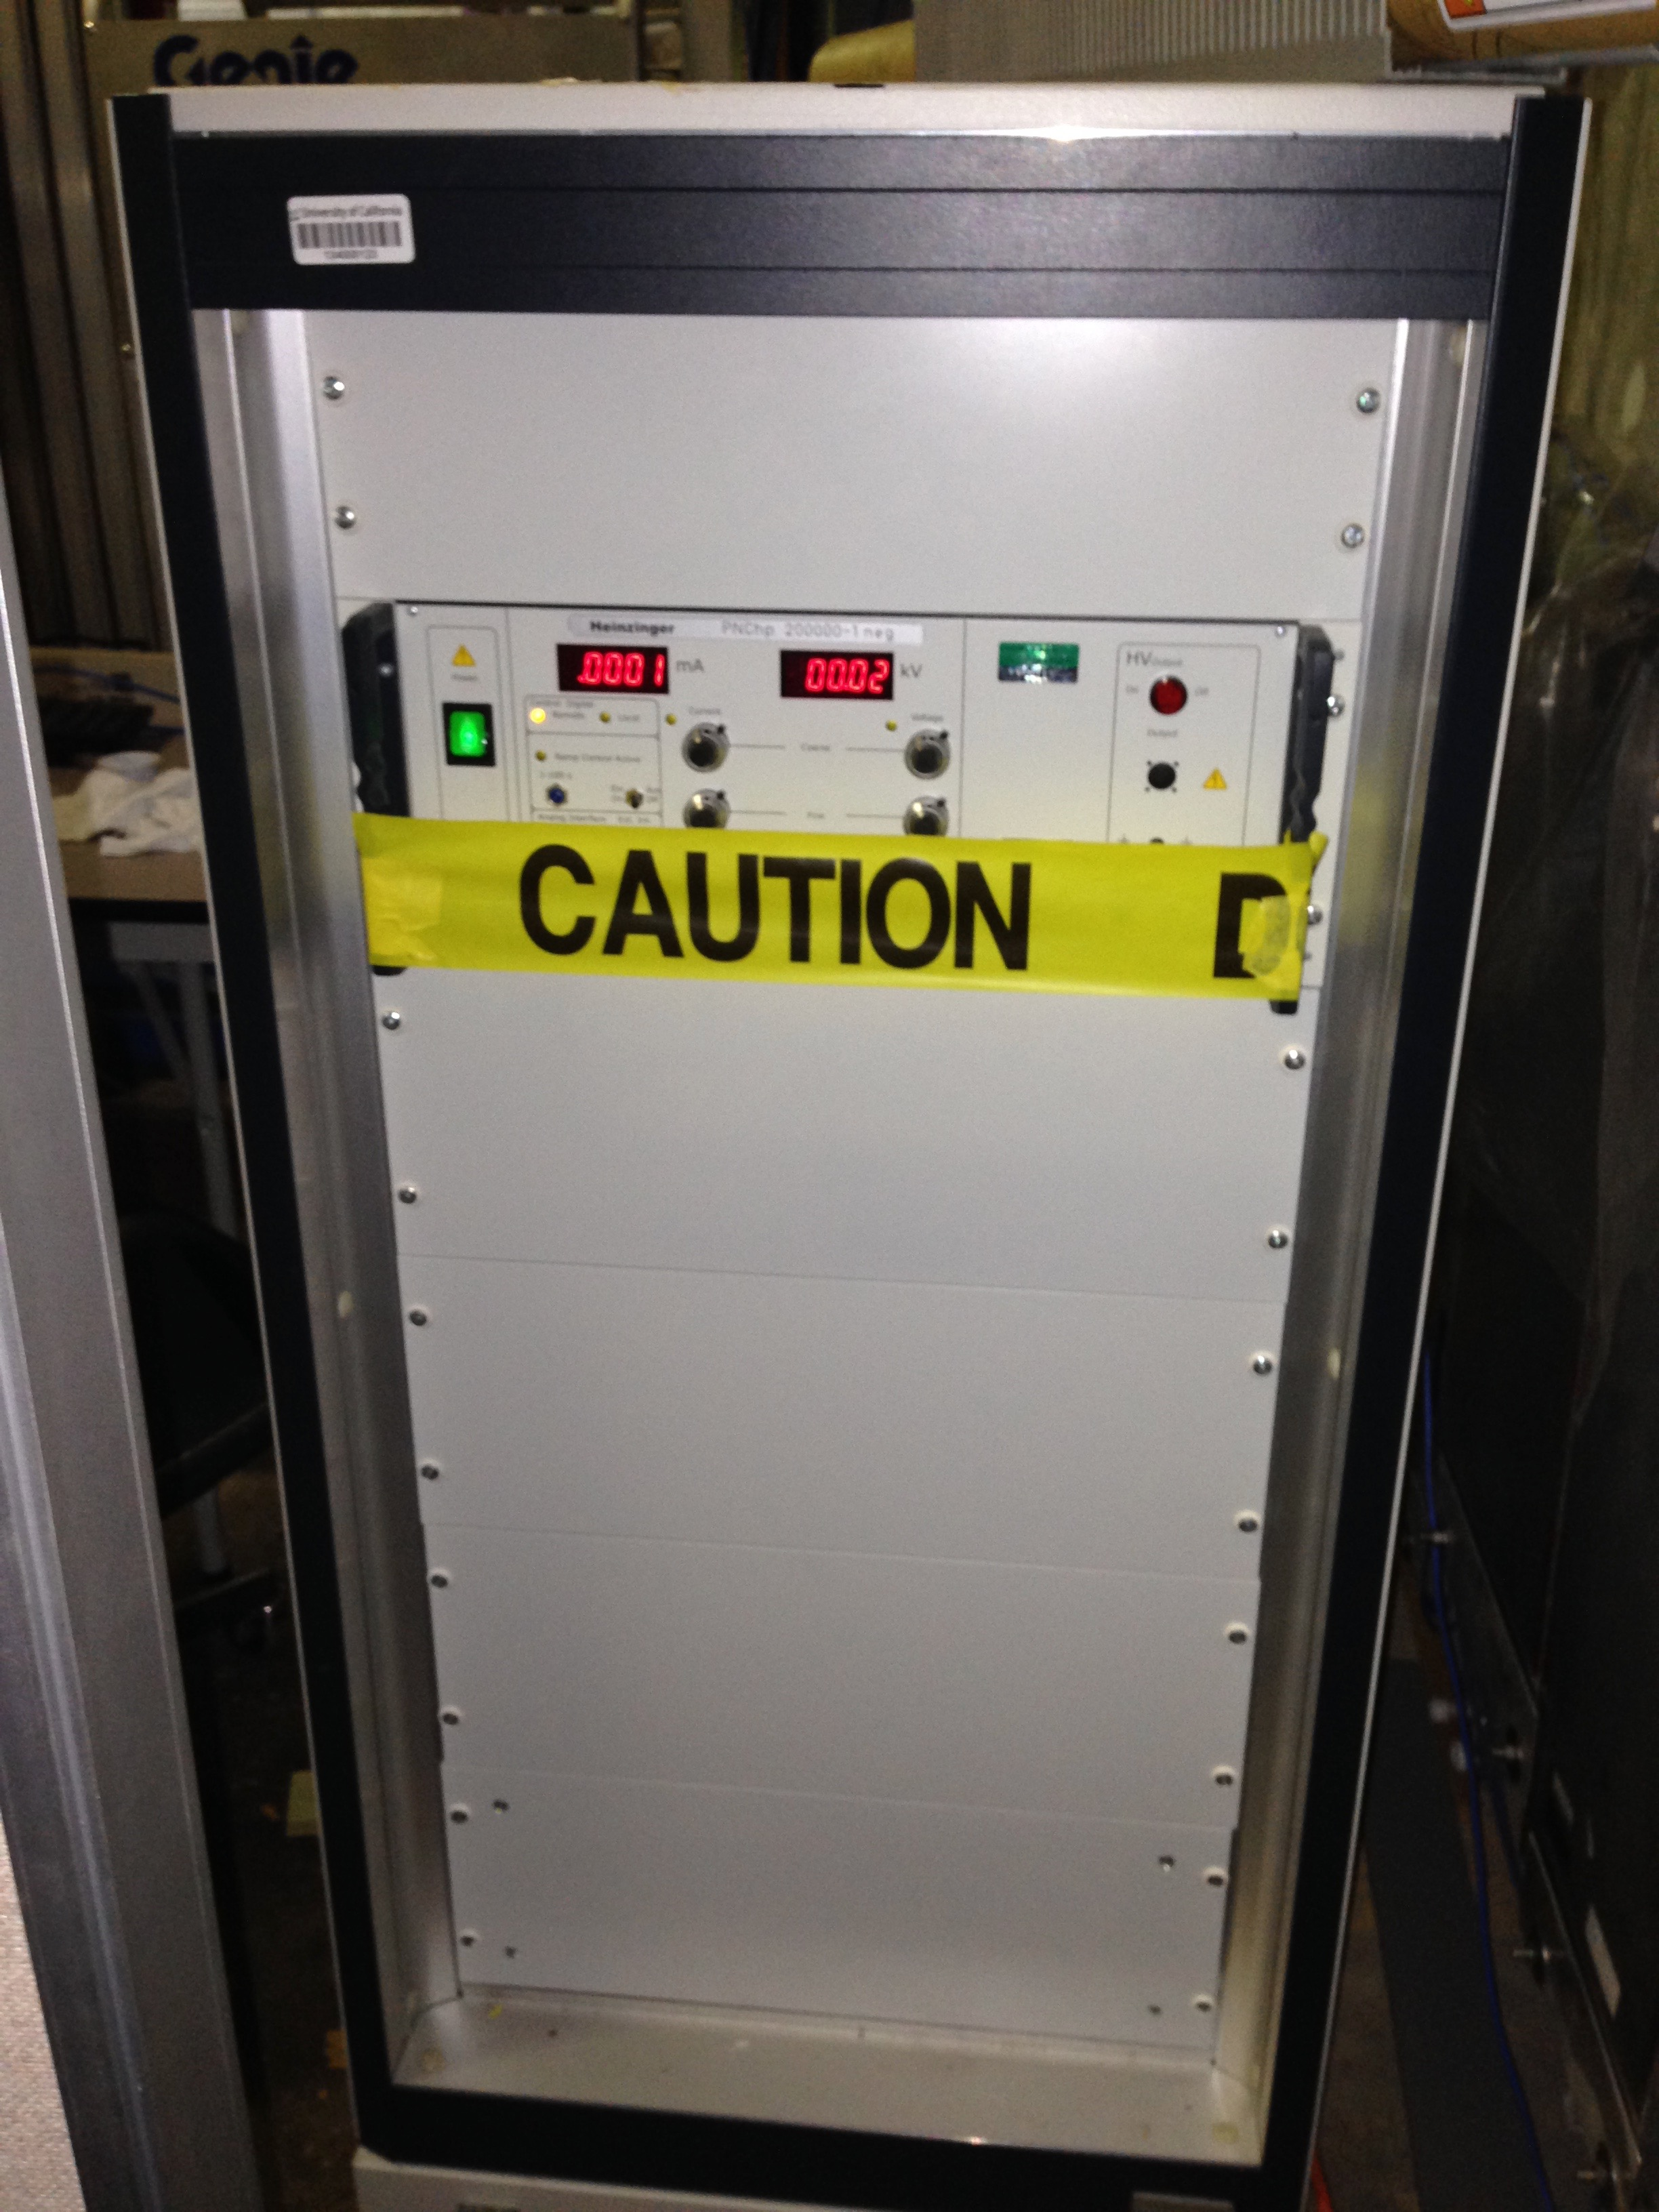
\includegraphics[width=0.2\textwidth]{heinzy}}}$
  \hspace*{.2in}
  $\vcenter{\hbox{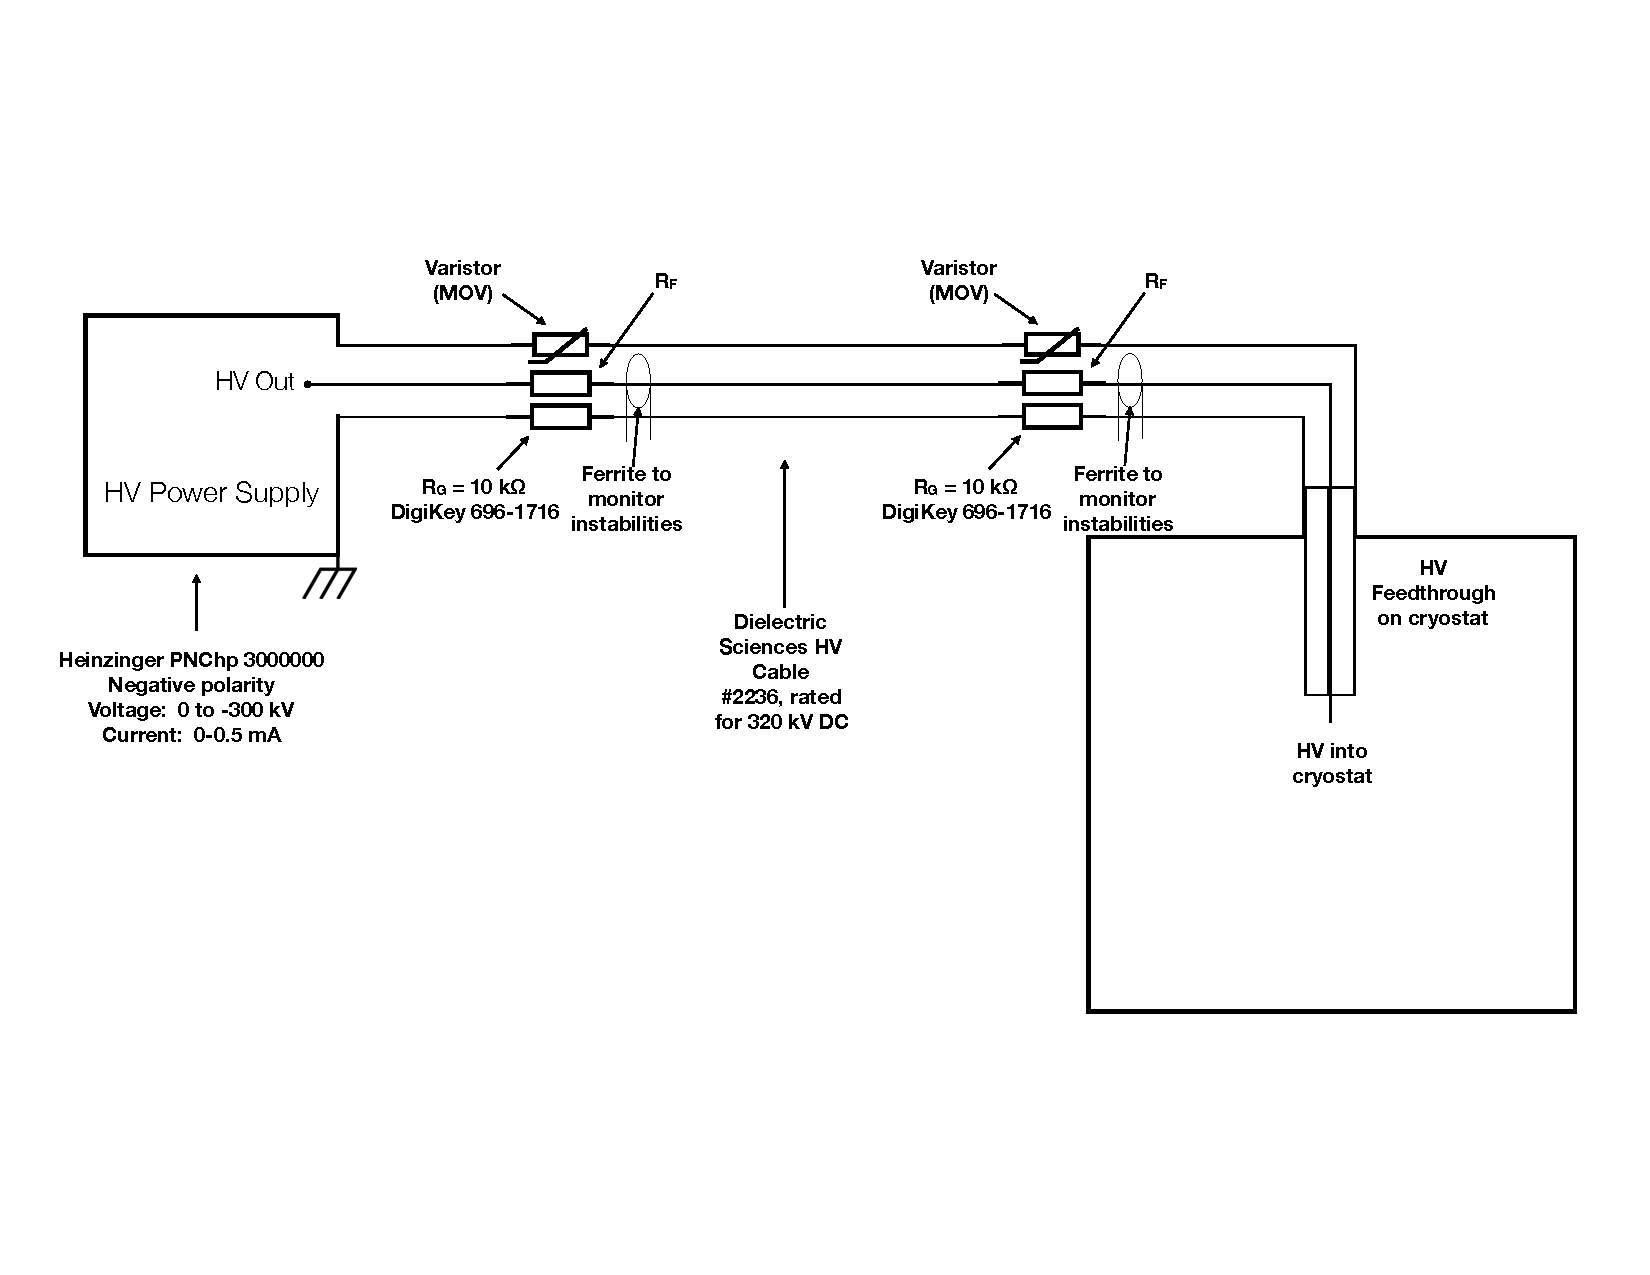
\includegraphics[width=0.7\textwidth]{ps_filter_ft_schematic}}}$
\end{minipage}
\end{dunefigure}
The requirement %of 
on low electronics noise sets the upper limit of residual voltage ripple on the cathode to be \SI{0.9}{mV}.  Typically, commercial supplies %can 
specify  that the ripple variation is limited to % less than or equal to $0.001\%V_{nom} \pm 50$ mV.  
\SI{.0001}{\%} around an absolute precision in nominal voltage of plus or minus \SI{50}{mV}.
%
Assuming cable lengths of \SI{30}{m} and \SI{3}{m} between the filters themselves, and between the filter and \fdth, respectively, resistances as low as a few \si{\mega\ohm} yield the required noise reduction according to calculations and experience. % the noise reduction can be attained with resistances as low as a few M$\Omega$. 

The current plan for the filters is a cylindrical design.  %Here, an \dword{hv} resistor will be electrically connected on each end to a cable receptacle.  
Here each end of an \dword{hv} resistor is electrically connected to a cable receptacle. 
The resistor %should shall be selected to 
must withstand a large over-power condition.  Radially out from the resistor is an insulator,  %In other designs, this has been 
for which other designs have used transformer oil or ultra-high molecular weight polyethelene (UHMWPE).  The outer case of the filter is a grounded stainless-steel or aluminum shell. The filter design used for ProtoDUNE-SP is shown in Figure~\ref{fig:filterAndFeedthrough}.

The \dword{hv} feedthrough %will be 
is based on the successful ICARUS design, \fixme{ref} which has been adapted for \dword{pdsp}.  The voltage is transmitted by a stainless steel center conductor.  On the warm side of the cryostat, this conductor mates with a cable end.  Inside the cryostat, the end of the center conductor has a spring-loaded tip that %will 
contacts a receptacle cup mounted on the cathode, delivering \dword{hv} to the field cage.  The center conductor of the \fdth is surrounded by UHMWPE. A drawing is shown in Figure~\ref{fig:filterAndFeedthrough}.

\begin{dunefigure}[Drawings of the \dword{hv} filters and feedthroughs]{fig:filterAndFeedthrough}
{Left:  Drawing of a \dword{hv} filter (Credit:  A.~Renshaw). Right:  \dword{hv} feedthrough drawing (Credit:  (F.~Sergiampietri).}
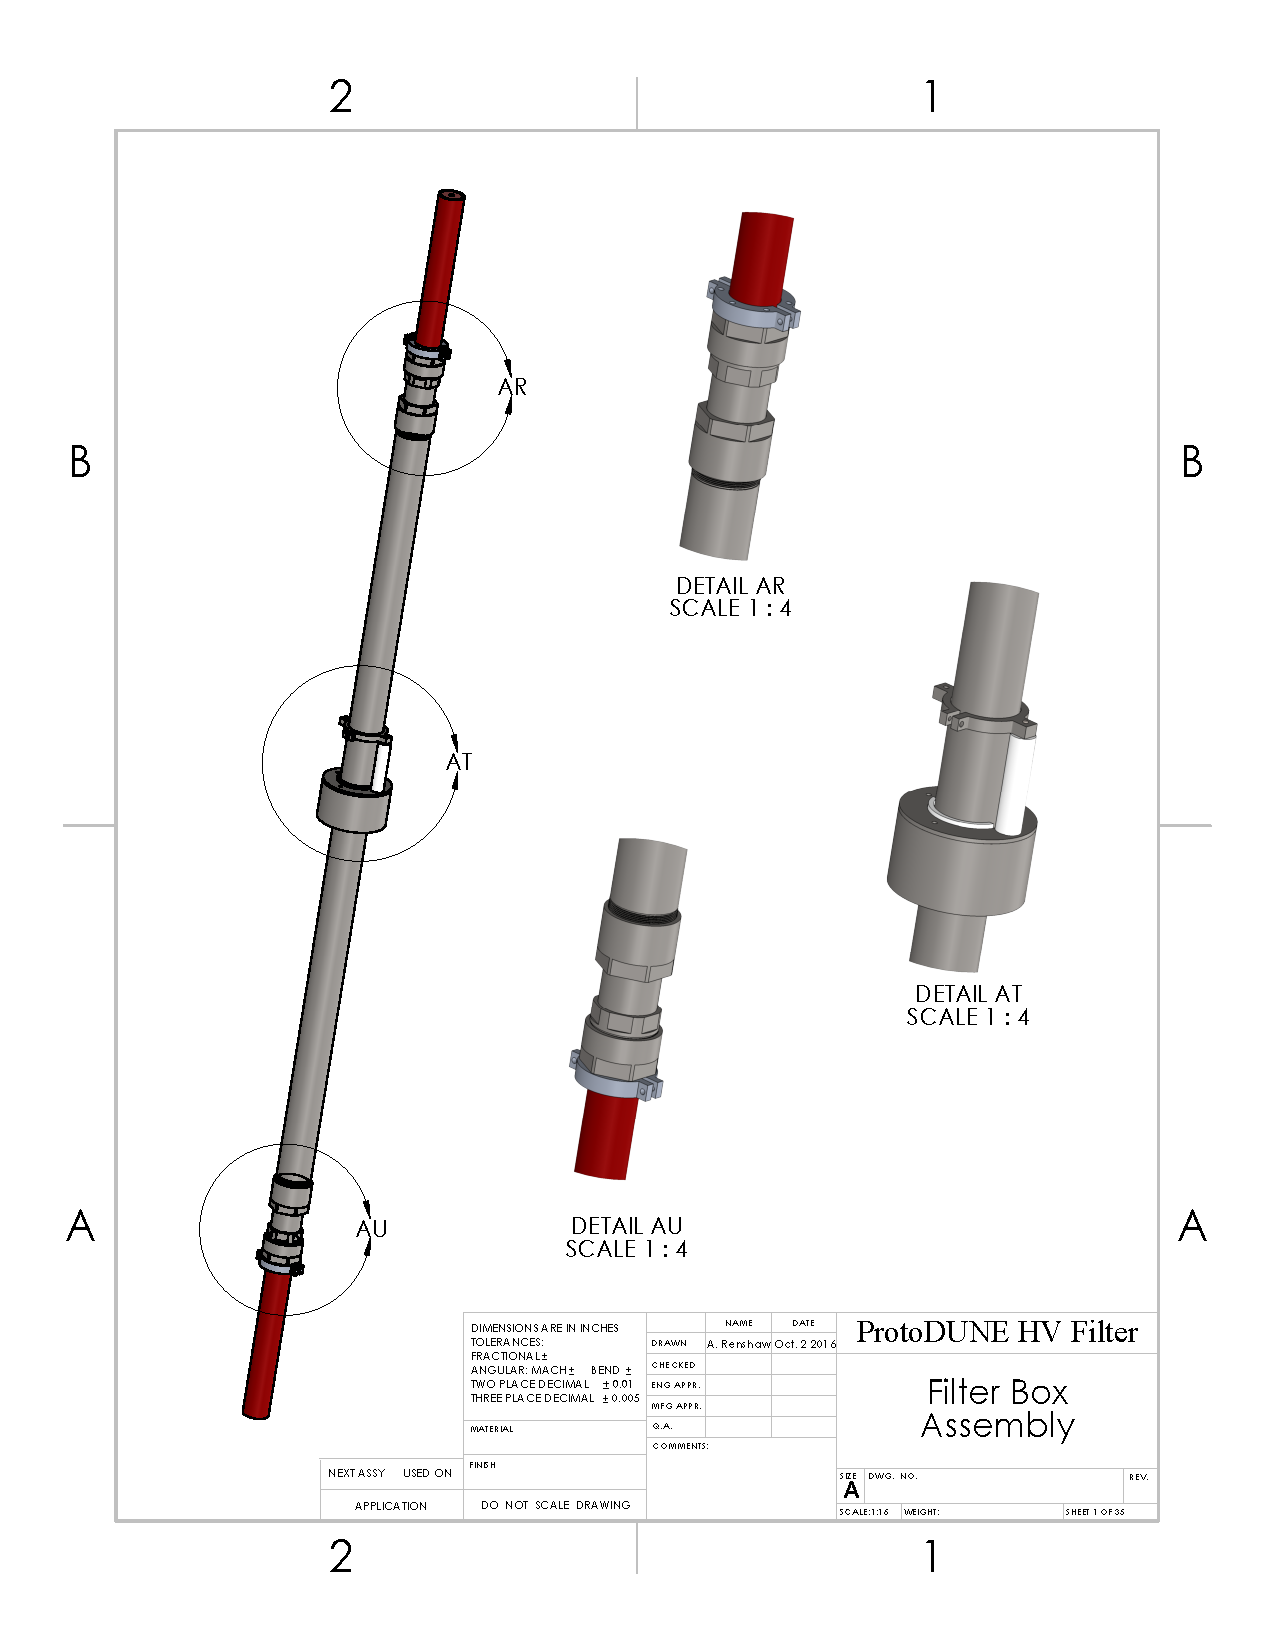
\includegraphics[width=0.3\textwidth]{pdFilters}
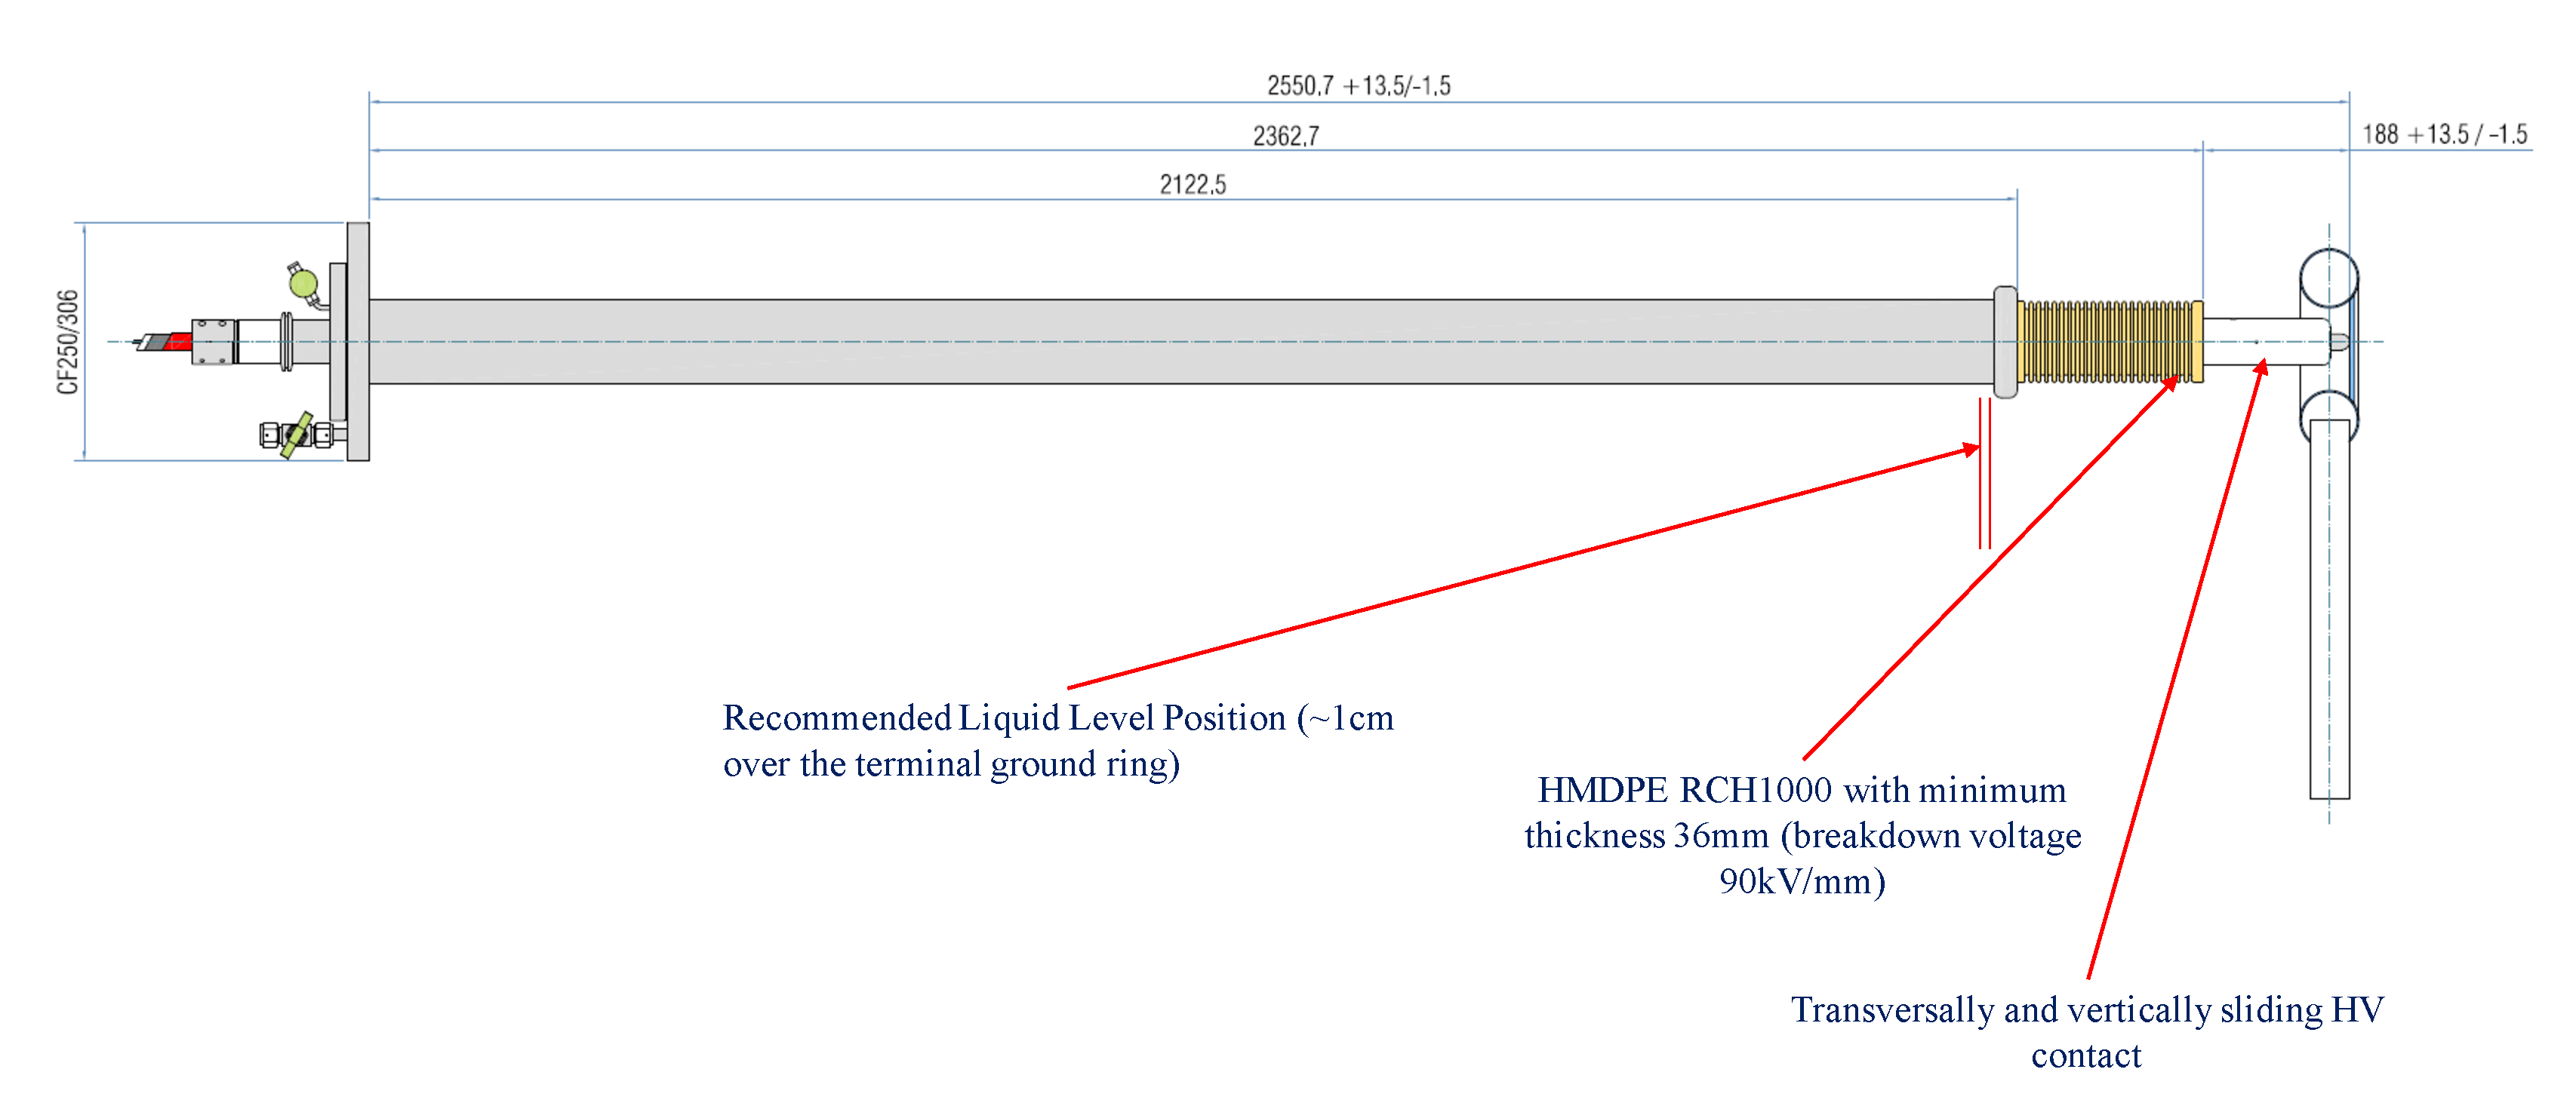
\includegraphics[width=0.6\textwidth]{francosHVFT}
\end{dunefigure}

The upper bound of operating voltage on a feedthrough is, to first order, set by the maximum \efield{} on the feedthrough.  This \efield{} is reduced by increasing the insulator radius.  For the target voltage, the feedthrough uses a UHMWPE cylinder of approximately \SI{15}{cm} diameter.  In the gas space and into at least \SI{15}{\centi\meter} of the liquid, the insulator is surrounded by a tight-fitting stainless steel ground tube.  The ground tube has a %\SI{25}{\centi\meter}  
Conflat (an industry standard) flange  welded on for attachment to the cryostat.

%Orig pgraph
%There will be multiple devices used to monitor the \dword{hv}.  Outside of the cryostat, the power supply and cable-mounted toroids will be used.  The Power Supply units typically have sensitivities down to 10's of nA in current read-back capability.  The units are able to sample the current and voltage every \SI{300}{ms}.  The cable-mounted toroids are sensitive to fast changes in current and can be monitored when desired.  The polarity of the signal also points to whether the current-drawing feature is upstream or downstream of the toroid.

Outside of the cryostat, the \dword{hv} power supply and cable-mounted toroids will monitor the \dword{hv}.    The power supplies %units 
typically have sensitivities down to tens of \si{\nano\ampere} in current read-back capability 
%\fixme{`in read-back `mode'? or `with' read-back capability? RKP: Believe language clear as written.} 
and are able to sample the current and voltage every \SI{300}{\ms}.  The cable-mounted toroids are sensitive to fast changes in current; %and can be monitored. when desired.  
the polarity of a toroid's signal %also points to whether 
indicates the location of the current-drawing feature as either upstream or downstream of it.  Experience from the \dword{35t} installation suggested sensitivities to changing currents with a timescale between \SIrange{0.1}{10}{\micro\s}, providing information on the timescale of any current changes.

Inside the cryostat, pick-off points near the anode will monitor the current %going down 
in each resistor chain.  Additionally, the voltage of the \dwords{gp} above and below each drift region can be equipped to diagnose problems via a high-value resistor connecting the \dword{gp} to the cryostat.  In the \dword{35t}, such instrumentation provided useful information on \dword{hv} stability and where any stray charge was flowing.

%The external commercial \dword{hv} components will be rated at a sufficient voltage to meet the drift voltage requirement (number 1 as listed in Table~\ref{tab:hvphysicsreqs}).  Additionally, the custom filters and feedthrough will be tested to ensure that they satisfy requirement (1).  Further details 
Both commercial and custom \dword{hv} components must be rated for sufficient voltage and satisfy tests to meet the requirements summarized in Table~\ref{tab:hvphysicsreqs}.  Further details on these tests are in Section~\ref{sec:fdsp-hv-qc}.

The resistances in the filters, in combination with the capacitances between the \dword{hv} system and the cathode,
 determine the attenuation of the tens of \si{\kilo\hertz} ripple from the power supply.  The filters %will be 
are designed such that the ripple is reduced to an acceptable level when installed in the complete system, thus satisfying requirement (3) that the power supply ripple is minimized.
%`\fixme{`minimize ripple'' is not a validatable requirement. What is the acceptable level? Or what dictates it? Anne. RKP: Addressed in collaboration comments.}

%%%%%%%%%%%%%%%%%%%%%%%%%%%%
\subsection{Cathode Plane Assembly (CPA)}
The \dword{cpa} provides a constant potential surface at \SI{-180}{\kV} for the \dword{spmod}.  It receives its \dword{hv} from the feedthrough that makes contact with the \dword{hv} bus mounted on the \dword{cpa} frame through an attached donut assembly attached to the frame, as shown in Figure~\ref{fig:donut_cpa}. % shows the connection of the \dword{hv} input donut to the \dword{hv} bus on the \dword{cpa} frame. 
There are 4 donut connections in the \dword{spmod}, one on each end of the two \dword{cpa} Arrays. The \dword{cpa} also provides \dword{hv} to the first profile on the top and bottom \dword{fc} elements and to the \dwords{ewfc} as well. %More d
Details on the electrical connections are found in Section ~\ref{sec:fdsp-hv-design-interconnect}.

\begin{dunefigure}[\dword{hv} input donut connection to \dword{cpa}]{fig:donut_cpa}{\dword{hv} input donut connection to \dword{cpa}.}
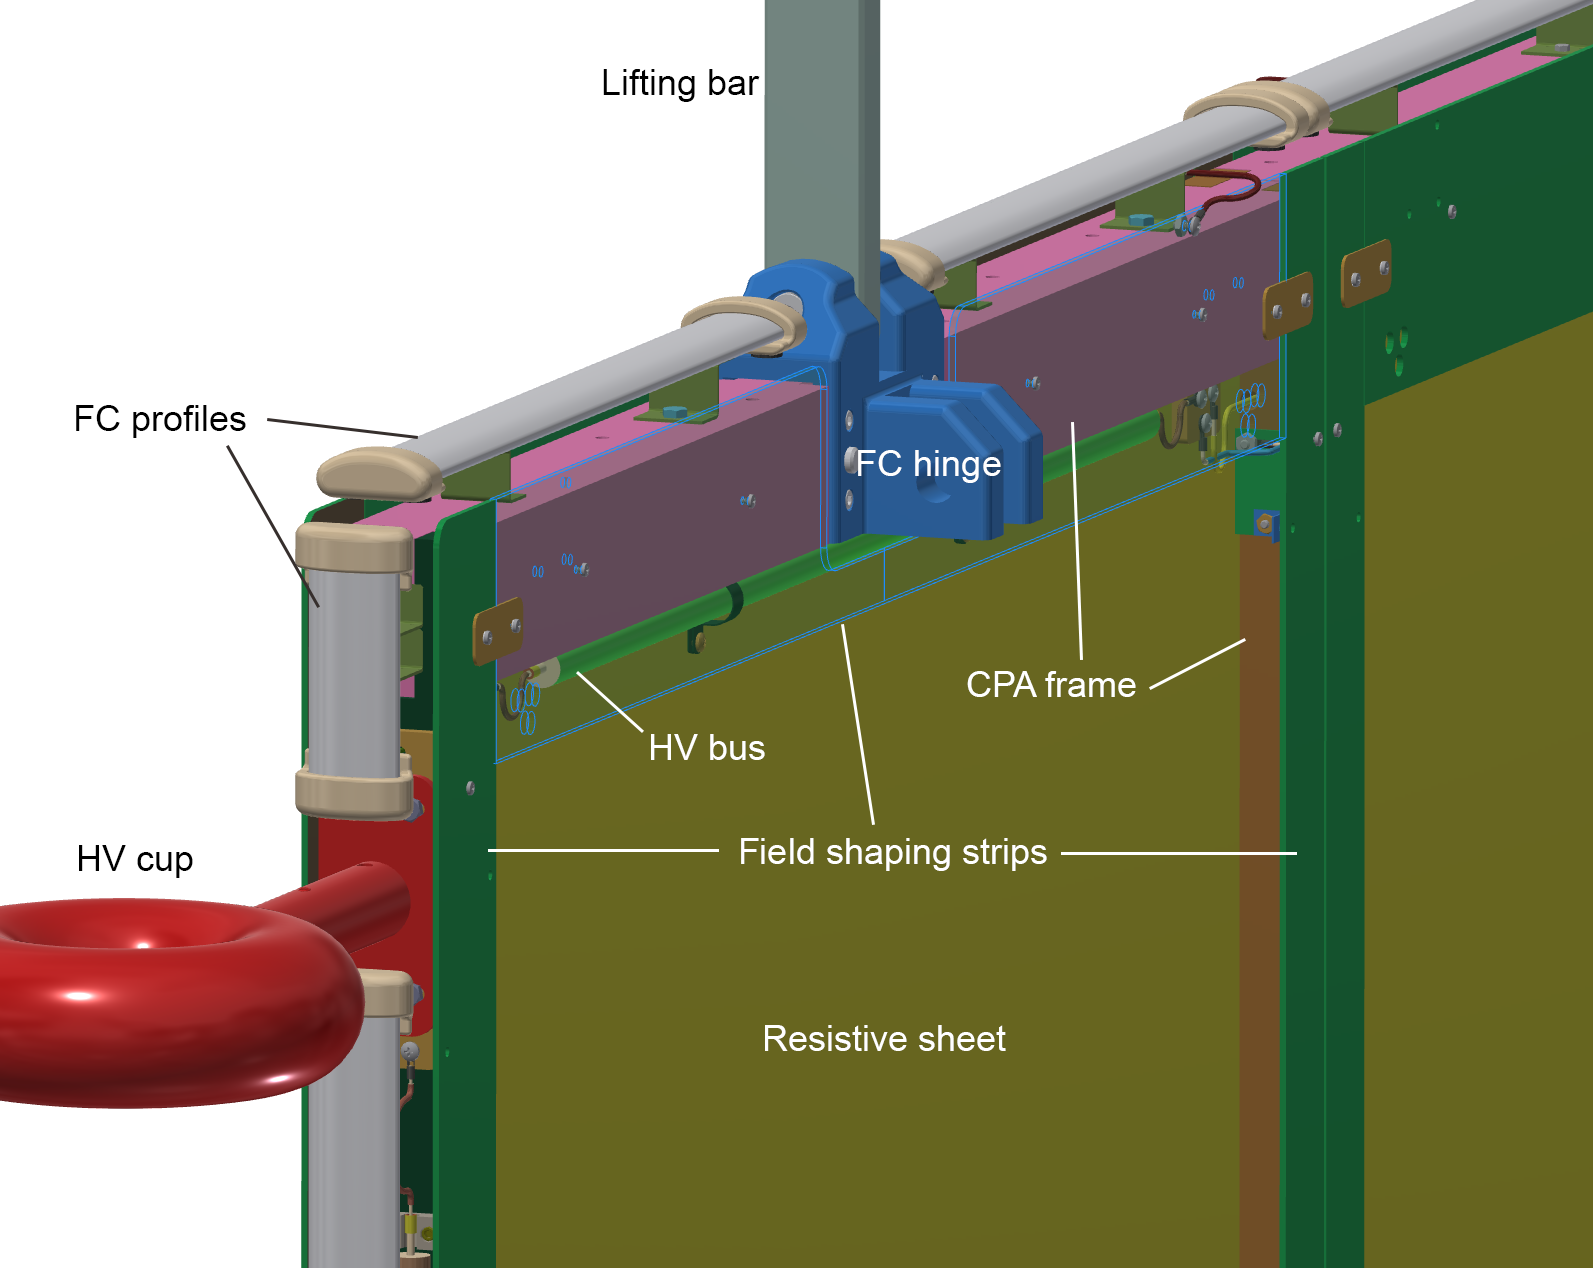
\includegraphics[width=0.6\textwidth]{donut_cpa2} %{ was Latest3D}
\end{dunefigure}

Ideally, the cathode would be constructed from a large thin resistive sheet.  However, inside the cryostat, there is a moderate convective flow of the \lar that can produce a small pressure difference across the cathode surface.  To maintain the position and flatness of the cathode, the cathode surface must be reinforced for stiffness.  This is accomplished using \SI{6}{cm} thick FR-4 frames at \SI{1.2}{m} intervals. Since FR4 is a good insulator at cryogenic temperature with a different dielectric constant that \lar, the presence of the frame causes a local \efield distortion that can become pronounced if the frame surface charges up as a reult from ionization in the TPC.  To minimize this distortion, a resistive field shaping strip is placed on the cathode frame and biased at a different potential.  Figure~\ref{fig:fss_concept} illustrates the drift field uniformity improvement with the field shaping strips.

\begin{dunefigure}[\dword{fss} concept]{fig:fss_concept}{A comparison of three cathode cross sections to illustrate the benefit of the \dword{fss}. Both equipotential lines (horizontal) and \efield{} lines (vertical) are shown.  The amplitude of the \efield{} is shown as color contours. Each color contour is a 10\% step of the nominal drift field.  The gray rectangles represent the frame and the resistive sheet in each case. Left: a conductive/resistive frame similar to that of ICARUS or SBND; Middle: an insulating frame with the insulating surfaces charged to an equilibrium state; Right: an insulating frame covered with a field shaping strip (purple) and biased at the optimum potential. }
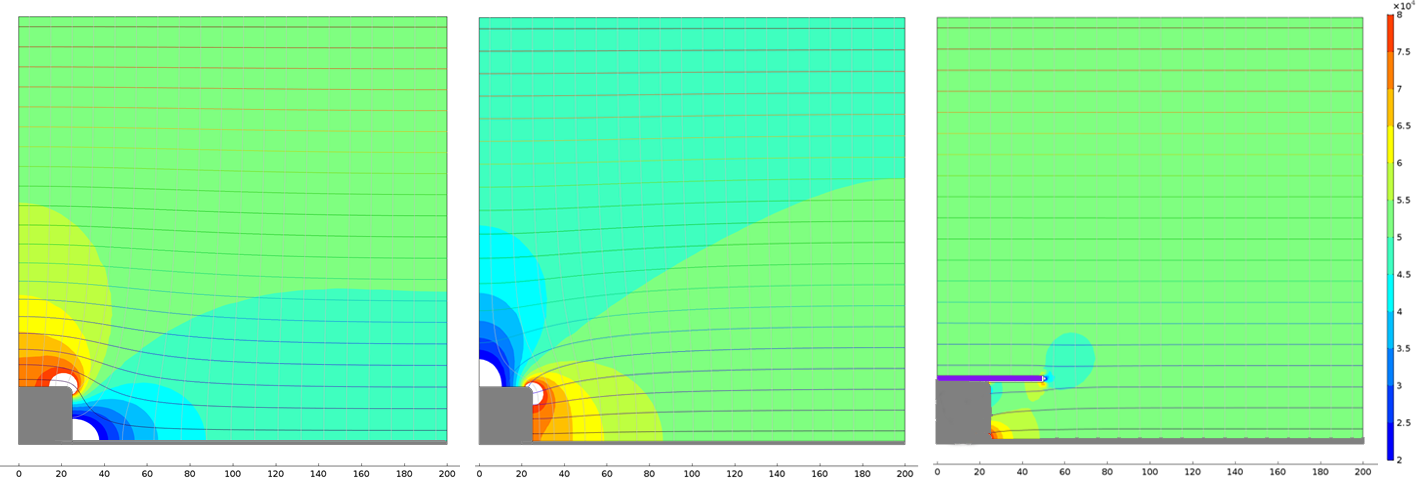
\includegraphics[width=0.9\textwidth]{field-shaping-strip-concept} %{ was Latest3D}
\end{dunefigure}

The \dwords{cpa}' constant potential surfaces are resistive panels (\dword{cpa} RPs) composed of a thin layer of carbon-impregnated Kapton\footnote{DuPont\texttrademark{}, Kapton\textsuperscript{\textregistered} polymide film,  E. I. du Pont de Nemours and Company,  \url{http://www.dupont.com/}.} 
 laminated to both sides of a \SI{3}{\milli\meter} thick FR4 sheet of \SI{1.2}{\meter}  $\times$ \SI{2}{\meter} size.  The surface resistivity of the \dword{cpa} RPs is required to be greater than 1 M\si{\ohm}/square in order to provide for slow reduction of accumulated charge in the event of a discharge.  A goal of 1 G\si{\ohm}/square for DUNE \dword{cpa} RPs extends the protection from discharges in the condition of anticipated higher stored energy at DUNE, compared to prototypes. Other \dword{hv} components of the \dword{cpa} include \dword{fss} mounted to the \dword{cpa} frames, edge aluminum profiles to act as the first elements of the field cage, and cable segments forming the \dword{hv} bus. Careful inspection of these items during the assembly process ensures that no sharp points or edges are present. The surface resistivity of the \dword{cpa} RPs and the \dword{fss} are checked multiple times during assembly -- first when the resistive panels and strips are received and after assembly into \dword{cpa} units on the table.  Coated parts that do not meet the minimum surface resistivity requirement are replaced.  This ensures that requirement (5) on Table~\ref{tab:hvphysicsreqs} is satisfied.  Figure~\ref{fig:cpa_panel-complete} shows a completed \dword{pdsp} \dword{cpa} panel on the production table ready for lifting into vertical position for mounting on its trolley.

\begin{dunefigure}[Completed \dword{pdsp} \dword{cpa} panel on production table]{fig:cpa_panel-complete}{Completed \dword{pdsp} \dword{cpa} panel on production table.}
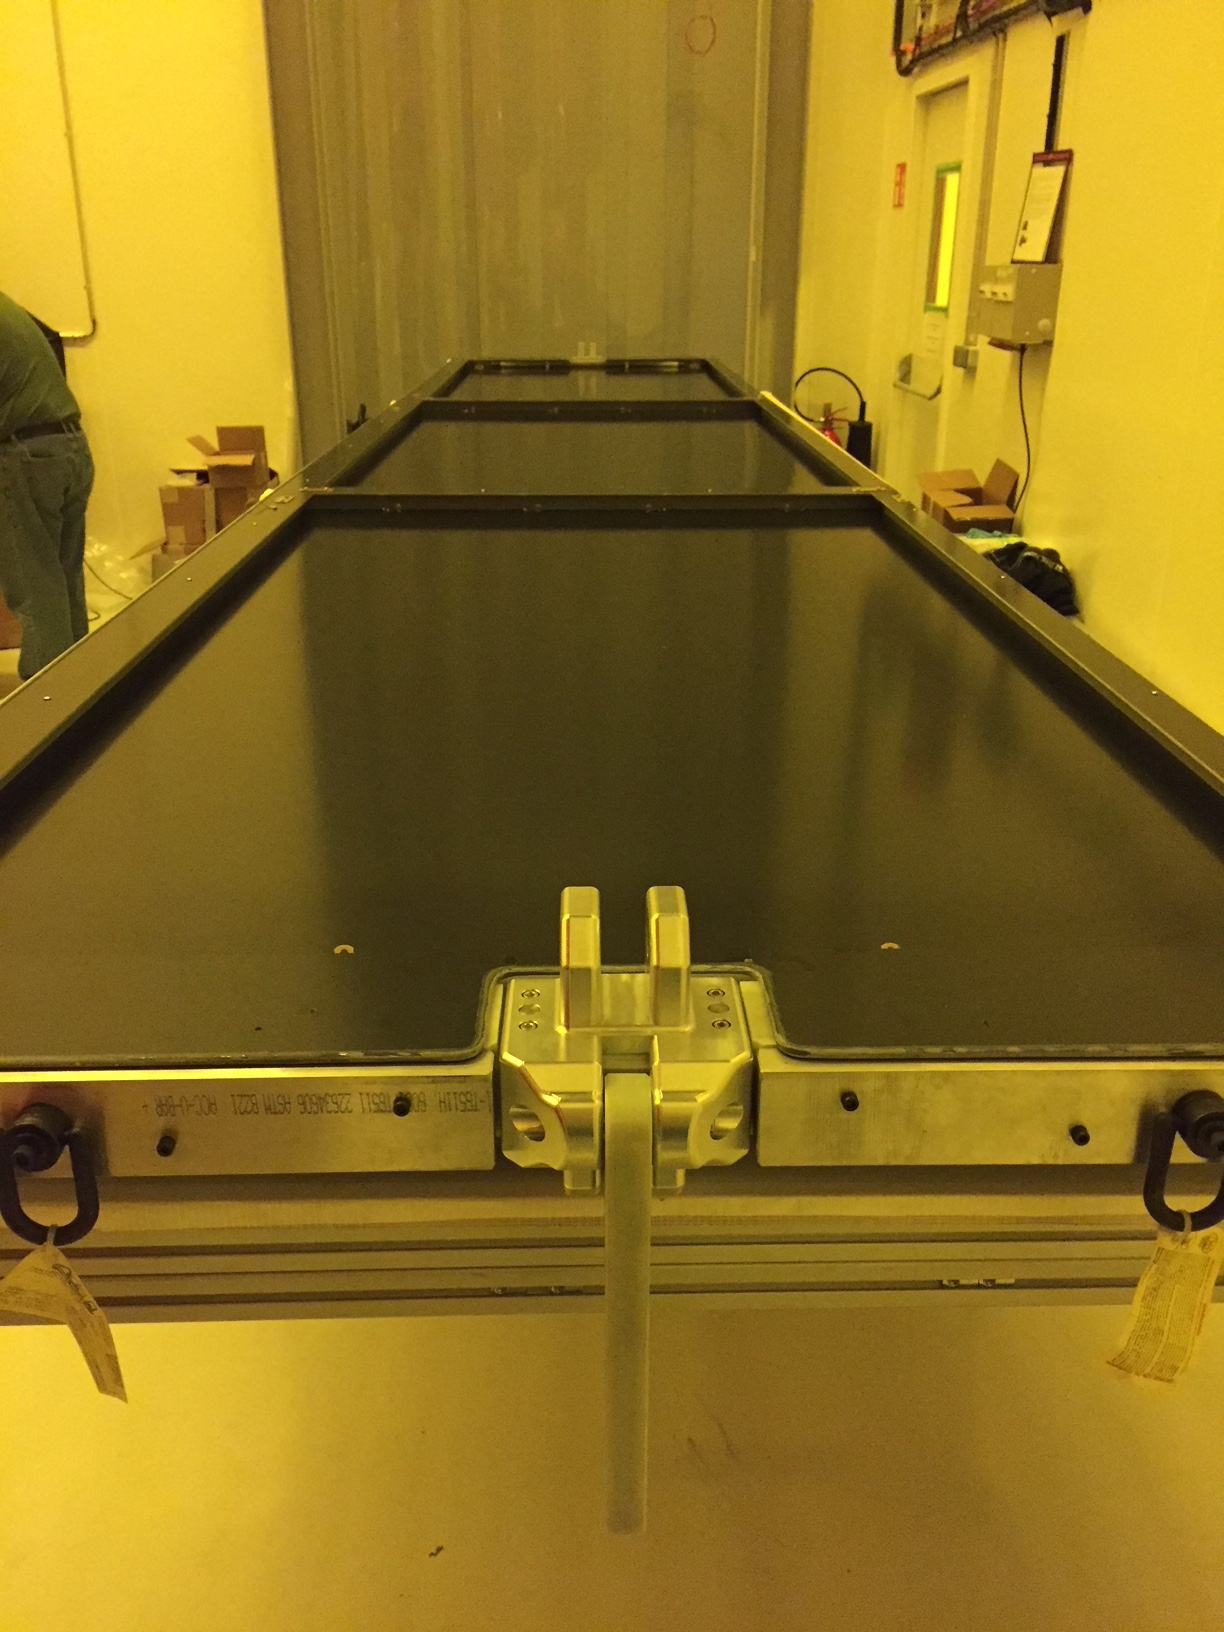
\includegraphics[width=0.5\textwidth]{cpa_panel-complete}
\end{dunefigure}

All electrical connections on the \dword{cpa} and between the \dword{cpa} and other \dword{hv} system components (top, bottom, and \dwords{ewfc}) are redundant by at least a factor of two.  Connections between RPs in a \dword{cpa} Unit are four-fold redundant.  The \dword{hv} connection from the \dword{hv} power supply is a closed loop around the \dword{cpa} which can sustain at least one broken connection without loss of the cathode plane \dword{hv}.  This ensures compliance with %that 
requirement (6) of Table~\ref{tab:hvphysicsreqs}.
%is satisfied.

The \dword{cpa} frames are required to support, in addition to the \dword{hv} components, the \dword{topfc} and \dword{botfc} units attached to both sides of the \dword{cpa} Plane. The arrangement and deployment of these components will be the same as in \dword{pdsp}.  

%%%%%%%%%%%%%%%%%%%%%%%%%%%%
\subsection{Field Cages}

\subsubsection{General Considerations}

A uniform \efield{} is required to drift ionization electrons towards the \dwords{apa}. The \dwords{fc} consisting of field shaping electrodes form a barrel surrounding the top, bottom, and ends of the active drift volume. The electrodes are biased at different potentials to establish a uniform field inside the \dword{lar} volume.
The \dword{spmod} will use extruded aluminum profiles as a cost-effective way to establish the equipotential surfaces. 

For safe and stable operation of the \lar cryogenic system, the cryostat must have a small fraction of its volume filled with gaseous argon, commonly referred to as the ullage. Since we want to make good use of the \lar in the cryostat, the top boundary of the TPC, the upper \dword{fc}, is not very far from the ullage. There are many grounded metallic components in the ullage with sharp features.  The \efield near these conductors could easily exceed the breakdown strength of gaseous argon. To prevent such breakdowns in the argon gas, a \dword{gp} is added above the upper \dword{fc} electrodes at a safe distance and below the liquid surface to shield the high \efield from entering the gas ullage.  The need for such shielding diminishes toward the \dword{apa} end of the \dword{fc} due to the lower voltages on the \dword{fc} profiles in that region. Therefore the \dword{gp} on the top only covers about \SI{70}{\%} of the \dword{cpa} side of the \dword{fc}, leaving extra room for cable routing near the \dwords{apa}.
On the bottom of the cryostat, a similar set of \dwords{gp} is planned to prevent breakdown, in the liquid, to cryogenic pipings and other sensors with sharp features.  No \dwords{gp} are planned beyond the two \dwords{ewfc} since there is sufficient clearance in those regions.  

The shape of the electrodes is critical as it determines the strength of the \efield{} between a given profile and its neighboring profiles, as well as
other surrounding parts, including the \dword{apa}, which is electrically at ground. % level. 
Electric fields need to be well below \SI{30}{\kilo\volt/\centi\meter} 
to satisfy design requirement (2) and enable safe \dword{tpc} operation~\cite{Blatter:2014wua}. % [A. Blatter, et al., JINST 9 (2014) P04006] %(design requirement 2).

The commercially available profiles used for \dword{pdsp}, and forming the \dword{spmod} design, are estimated to lead to \efield{}s of up to \SI{12}{\kilo\volt\per\centi\meter} under the %assumption of DUN\efield{} cage configuration 
%and operating voltage. 
configuration and operating voltage assumptions.
Figure~\ref{fig:profile-e-field} illustrates results from an \efield{} calculation.
%%% After last commit 3/29 1:45 ish Anne
\begin{dunefigure}
[\efield map and equipotential contours of profiles at \SI{-180}{\kV}]{fig:profile-e-field}
{\efield map (color) and equipotential contours of an array of roll formed profiles biased up to \SI{-180}{\kV} and a ground clearance of \SI{20}{\cm}(Credit: BNL CAD model).} 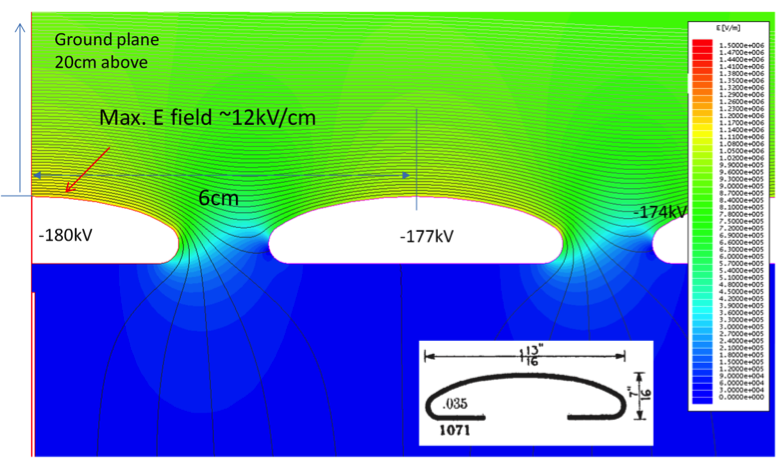
\includegraphics[width=0.8\textwidth]{profile-e-field.png}
\end{dunefigure}

The profiles ends are equipped with UHMW polyethylene caps to reduce the risk of arc formation.  These caps are designed to have sufficient wall thickness (\SI{6}{\milli\m}) to withstand the full voltage across their walls.

The aluminum profiles are attached to fiber-reinforced plastic (FRP) pultruded structural elements, including I-beams and box beams.  
Pultruded FRP material is non-conductive and strong enough to withstand the \dword{fc} loads  in the temperature range of \SI{-150}{C} and \SI{23}{C}, as certified by vendors. Testing of the FRP joints were conducted at liquid nitrogen temperatures (see DocDb 1504).  The strength of the material increased over room temperature tests which provides confidence in the material behavior at \lar  temperature. 
%%%--- DUPLICATION ---%%%  Tests of FRP joints at LN temperature\fixme{ add citations in bib: CPA and FC Design, DUNE DocDB 1504} showed that the strength of the material increases at cryogenic temperature relative to room temperature, providing confidence in FRP material behavior at LAr temperature.
%FRP has all of the reinforcing fibers running along the main axis of the section being used.  
The FRP material meets class A standards for fire and smoke development established by the International Building Code characterized by ASTM E84\footnote{\textit{Standard Test Method for Surface Burning Characteristics of Building Materials}, ASTM International, \url{https://compass.astm.org/EDIT/html_annot.cgi?E84+18}.}

As discussed in Section~\ref{sec:fdsp-hv-intro}, %the Introduction, 
the field cage modules are of two types: the top and bottom \dword{fc} and the \dword{ewfc}, both of which are described below. 
A resistive divider chain interconnects all the aluminum profiles to provide a linear voltage gradient between the cathode and anode planes.  The top and bottom modules are nominally \SI{2.3}{\m} wide by \SI{3.5}{\m} long. A \dword{gp}, in the form of tiled, perforated stainless steel sheet panels, is mounted on the outside surface of the T/B field cage module with a \SI{20}{\cm} clearance. The top and bottom \dword{fc} modules are supported by the \dwords{cpa} and \dwords{apa}. The \dword{ewfc} modules are \SI{1.5}{\m} tall by \SI{3.5}{\m} long. They are stacked eight units high (\SI{12}{\m}), and are supported by the installation rails above the \dwords{apa} and \dwords{cpa}.

The \dwords{fc} are designed to produce a uniform electric field with understood characteristics.
The current (i.e., \dword{pdsp}) \dword{fc} design has a large gap between the \dword{ewfc} module and its neighboring top and bottom modules to allow the latter to swing past the \dword{ewfc} during the \dword{fc} deployment. This gap causes the largest known distortion in the electric drift field in the \dword{tpc}. Figure~\ref{fig:fc-distortion} shows the extent of the distortion in this limiting scenario. In \dword{pdsp}, the gap produces two regions (of total \lar mass \SI{20}{kg}) in the TPC near both bottom corners that suffer \SI{5}{\%} \efield distortions.

\begin{dunefigure}[Electric field at edge of \dword{fc}]
{fig:fc-distortion}
{\efield at a corner between the bottom and endwall \dword{fc} modules, showing effects of a \SI{7}{cm} gap. Left: the extent of \num{5}\% \efield{} non-uniformity boundary (black surface, contains less than \SI{10}{kg} of \lar) and \num{10}\% non-uniformity boundary (white surface, contains $\sim$ \SI{6}{kg} of \lar) inside the TPC's active volume. The inset is a view from the CAD model.  Right: electron drift lines originating from the cathode surface.}
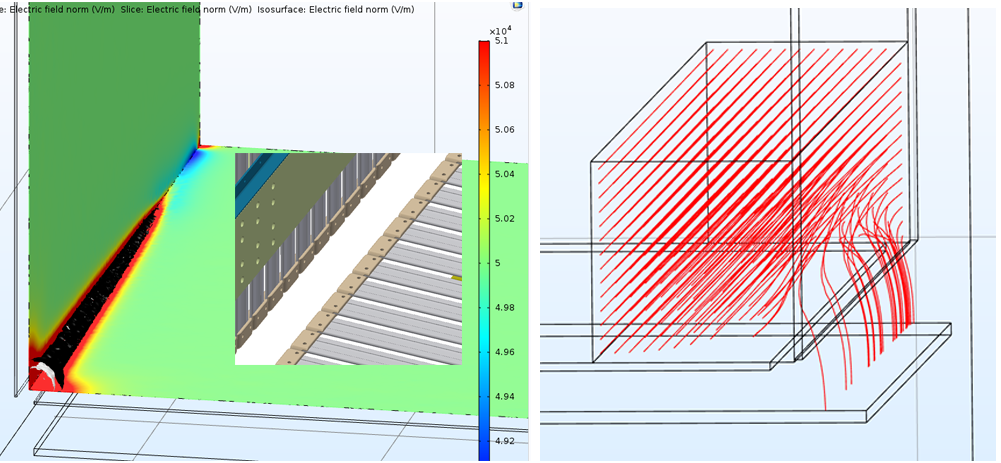
\includegraphics[width=0.9\textwidth]{distortion_from_fc_gap}
\end{dunefigure}

The \dwords{fc} %have been 
are designed to %ensure they 
meet the system requirements specified in Table~\ref{tab:hvphysicsreqs}. All components other than the aluminum profiles, \dwords{gp}, and electronic divider boards are made of insulating FRP and FR4 materials, and the end of each profile is covered with a UHMWPE end cap, to allow the system to reach the design \dword{tpc} \efield{} (requirement 1). The profiles have been carefully modeled to study the resulting \efield{}, and small-scale laboratory tests have been conducted to ensure that the maximum \efield{} does not approach \SI{30}{\kV\per\cm} (requirement 2). These design features are expected to avoid sparking, and thus to draw very small stable currents, which should produce a consistent load on the power supply (requirements 3, 4, and 5). Finally, all voltage divider boards provide redundany for establishing the profile-to-profile potential differences with only minor distortions to the E field in case of failure of any individual part, and two redundant boards provide the connection from the \dwords{fc} modules to the \dword{cpa} (requirement 6).

\subsubsection{Top and bottom field cages}

The \dword{topfc} and \dword{botfc} modules are \spfcmodlen{} long, which is set by the length of the two \SI{15.2}{\cm} (\SI{6}\,in) FRP I-beams that form the primary support structure of the modules. The I-beams are connected to each other by three  \SI{7.6}{\cm} (\SI{3}\,in) FRP cross beams. The connections between the longitudinal and cross I-beams are made with L-shaped FRP braces that are attached to the I-beams with FRP spacer tubes, and secured with FRP threaded rods, FRP hex-head nuts, and custom-machined FR4 washer plates.

The modules are \SI{2.3}{\m} wide, which corresponds to the length of the aluminum profiles, including the UHMW polyethylene end caps. Profiles are secured to the FRP frame using custom-machined double-holed stainless steel slip nuts that are slid into and electrically in direct contact with the Al profiles such that they straddle the webbing of the \SI{15}{\cm} I-beams, and are held in place with screws that penetrate the I-beam flanges. The profile offset with respect to the FRP frame is different for modules closest to the \dwords{ewfc}, %endwalls, 
and modules in the center of the active volume.

Each \dword{topfc} and \dword{botfc} module holds five ground planes, which are connected to the outside (i.e., the non-drift side) of the module. The \dwords{gp} are positioned $\sim$\SI{20.5}{\cm} above the profiles, and are pushed to the \dword{cpa} side of the module, leaving the last 14 profiles (\SI{88}{\cm}) on the \dword{apa} side of the module exposed. Between the \dwords{gp} and the \SI{15}{\cm} I-beams are standoffs made of short sections of \SI{10.2}{\cm} (4\,in)  FRP I-beams, which are connected with FRP threaded rods and slip nuts. The electrical connection between the ground planes is made with copper strips.

The connections between the top and bottom modules and the \dwords{cpa} are made with aluminum hinges, \SI{2.54}{\cm} (1\,in) in thickness, that allow the modules to be folded in to the \dword{cpa} during installation. The hinges are electrically connected to the second profile from the \dword{cpa}. The connections to the \dwords{apa} are made with stainless steel latches that are engaged once the top and bottom modules are unfolded and fully extended toward the \dword{apa}.

The voltage drop between adjacent profiles is established by voltage divider boards that are screwed into the drift volume side of the profiles. A custom-machined nut plate is used that can be inserted into the open slot of each profile and twisted \SI{90}{\degree} %$^\circ$ 
to lock into position. Two additional boards to connect the modules to the \dwords{cpa} were screwed into the last profile on the \dword{cpa}-side of the module. This system is also described in Section~\ref{sec:fdsp-hv-design-interconnect}. A fully assembled module is shown in Figure~\ref{fig:tbfc1-2}.

\begin{dunefigure}[Top and bottom field cage modules]{fig:tbfc1-2}{The fully assembled modules with ground planes are shown (left), as well as a close up of a \dword{cpa} end as viewed from the bottom (drift) side of the module.}
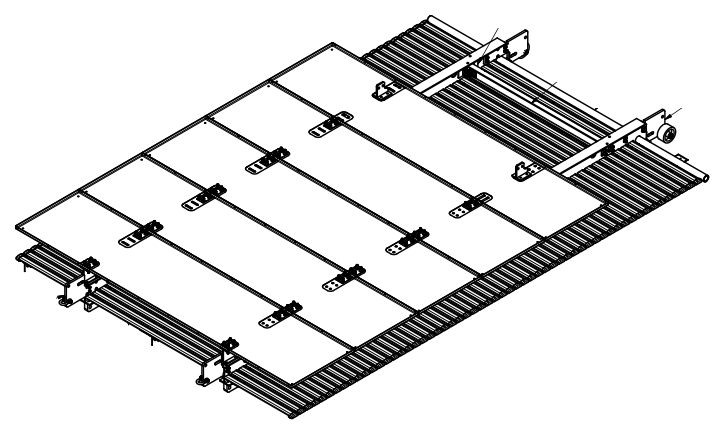
\includegraphics[width=0.65\textwidth]{tbfc1}
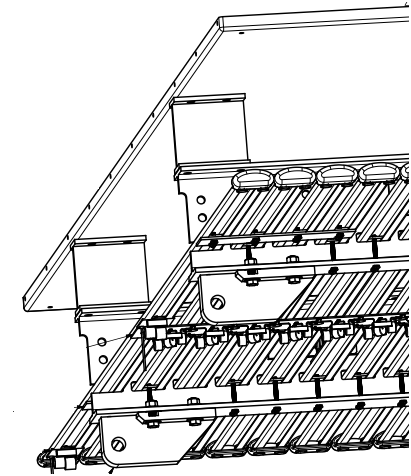
\includegraphics[width=0.33\textwidth]{tbfc2}
\end{dunefigure}

Between any two adjacent nodes of the resistor divider chain are two \SI{5}{\giga\ohm} resistors, and three serially connected metal oxide varistors (MOVs) in parallel.  The nominal voltage drop is \SI{3}{kV} between each node.
An open resistor on the divider chain would approximately double the voltage across the remaining resistor to \SI{6}{kV}.  This will force the varistors in parallel to that resistor into conduction mode, resulting in a voltage drop of roughly \SI{5}{kV} (\SI{1.7}{kV} $\times$ \num{3}), while the rest of the divider chain remains linear, with a slightly lower voltage gradient.
Because the damage to the divider would be local to one module, its impact to the \dword{tpc} drift field is limited to region near this module.  This is part of the intention of the modular design.
An example of a simulated \efield{} distortion which would be caused by a failed resistor is shown in Figure~\ref{fig:fc-broken-resistor}. 

\begin{dunefigure}[\efield distortion from broken voltage divider path]{fig:fc-broken-resistor}{Simulated \efield{} distortion from one broken resistor in the middle of the voltage divider chain on one bottom field cage module, emphasizing the need for redundancy. Left: Extent of \efield{} non-uniformity in the active volume of the TPC. the green planes mark the boundaries of the active volume inside the field cage. The partial contour surfaces represent the volume boundaries where \efield{} exceeds 5\% (dark red, contains less than 100\,kg of LAr) and 10\% (dark blue, contains less than 20\,kg of LAr) of the nominal drift field. Units are \si{\volt\per\m} in the legend. Right: electron drift lines connecting the \dword{cpa} to \dword{apa} in a bottom/end wall field cage corner.  The maximum distortion to the field line is about 5\,cm for electrons starting at mid drift at the bottom edge of the active volume.}
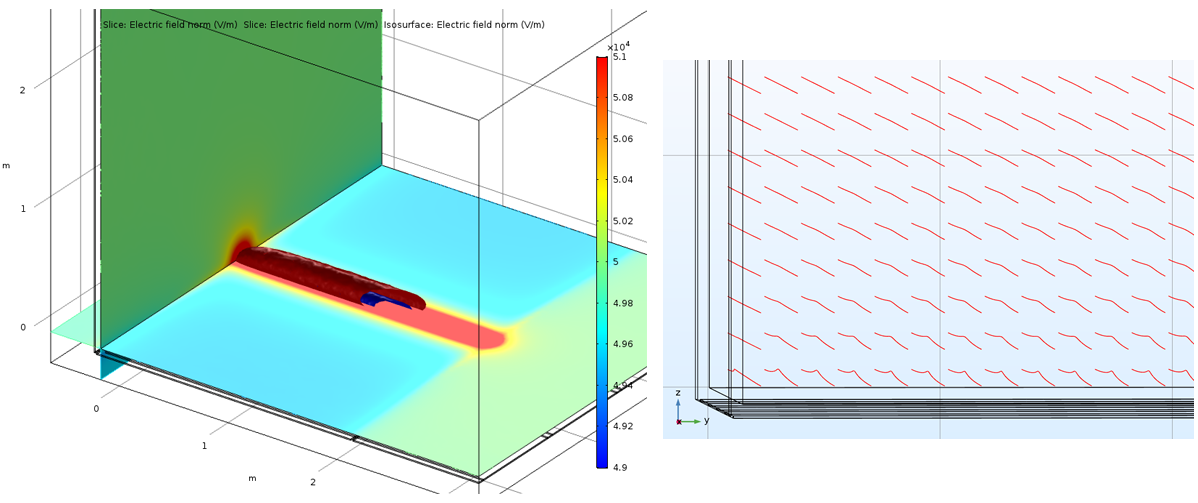
\includegraphics[width=0.9\textwidth]{e-field-distortion-due-to-open-resistor}
\end{dunefigure}
The effect of the non-uniformity in resistor values can also be scaled from this study.  A 2\% change in a resistor value (1\% change from the 2R in parallel) would give about 1.5\% of the distortion from a broken resistor, i.e. less than 1\,mm of transverse distortion in track position, with no noticeable drift field amplitude change inside the active volume.
 

\subsubsection{Endwall field cages (EWFC)}

%The endwall field cage (\dword{ewfc}) for each of the four drift volumes consists of two endwalls (EW), one on each side of the drift volume. Each endwall is in turn composed of eight endwall modules (EW-Modules). 

Each of the four drift volumes has two \dwords{ewfc}, one on each end. Each \dword{ewfc} is in turn composed of eight \dword{ewfc} modules.
There are two different types of \dword{ewfc} modules, each of which comes in a \textit{regular} and in a \textit{mirrored} configuration to account for 
mounting constraints and to match the detector geometry. Figure~\ref{fig:fc_endwall_panels} illustrates the layout for the topmost 
and the other panels, respectively.

\begin{dunefigure}[Endwall \dword{fc} panels]{fig:fc_endwall_panels}{Left: Uppermost panel of the \dword{ewfc}. Right: Non-uppermost \dword{ewfc} panel.}
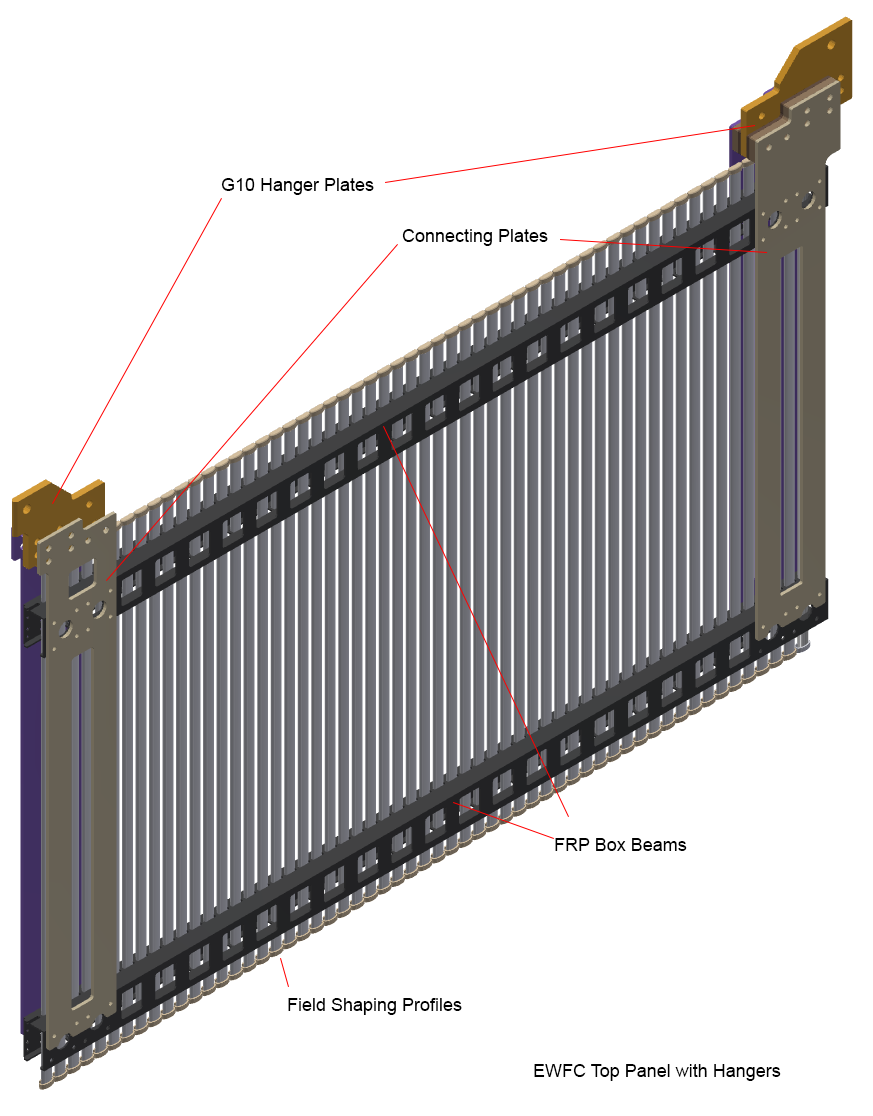
\includegraphics[width=0.48\textwidth]
{EWFC_Top_Module}
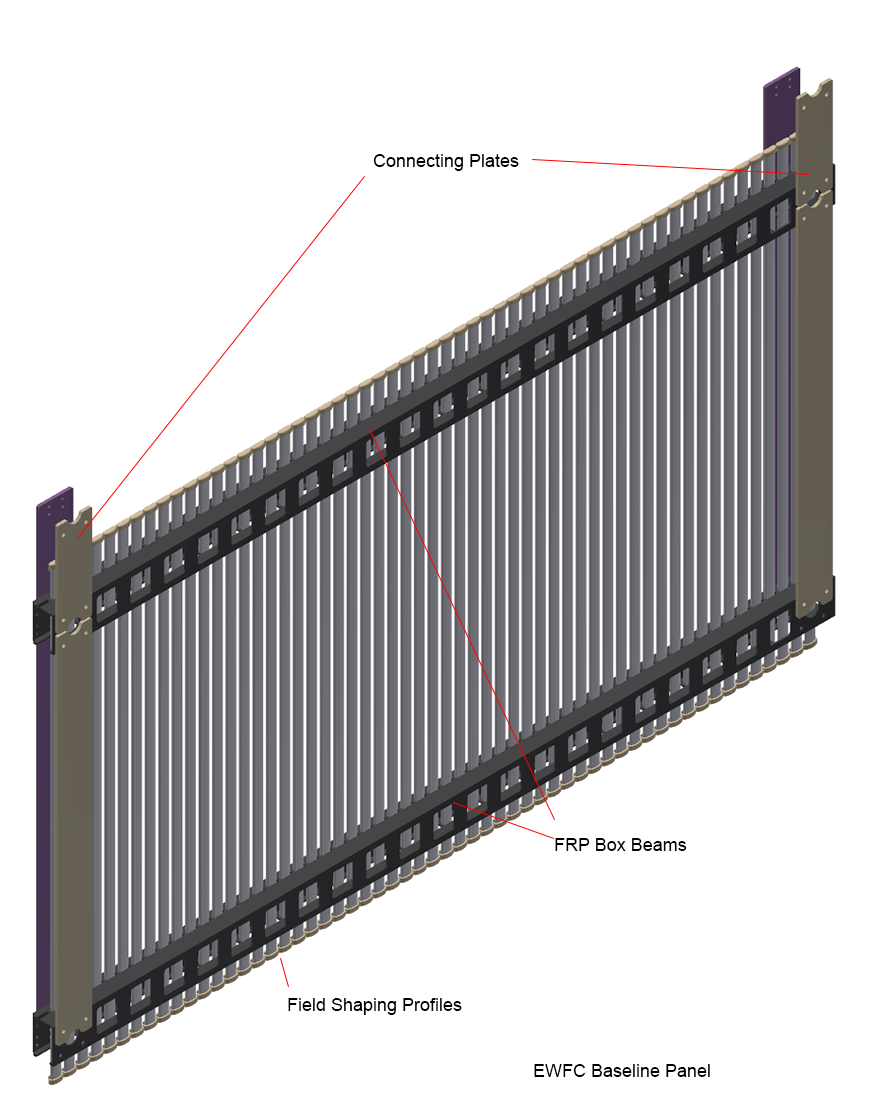
\includegraphics[width=0.48\textwidth]
{EWFC_Baseline_Module}
\end{dunefigure}

Each \dword{ewfc} module is constructed of two FRP box beams which are \SI{3.5}{\m} long. The box beam design also incorporates cutouts on the outside face to minimize charge build up. Box beams are connected using \SI{1.27}{\cm} (\num{0.5}\,in) thick FRP plates. The plates are connected to the box beams using a shear pin and bolt arrangement. The inside plates facing the active volume are connected using special stainless steel slip nuts and stainless steel bolts. The field-shaping profiles are connected to the top box beam using stainless steel slip nuts, an FRP angle, and two screws each which pass through matching holes in the wings of the Al profiles. At the bottom box beam the profiles are pulled against another FRP angle with a single screw and a slip nut that is held in place by friction.

%\begin{center}
%   \parbox[t]{0.47\textwidth}{
 %  \resizebox{0.47\textwidth}{!}{\includegraphics[width=0.48\textwidth]{\dword{fc}endwall_top-panel.png}}
%\caption{\label{fig:\dword{fc}endwall_top} Uppermost panel of the field cage endwall. {\color{red} NOTE: need to replace figure with updated version for DUNE, e.g. without middle FRP cross member.}}}
%\makebox[0.025\textwidth]{}
 %  \parbox[t]{0.48\textwidth}{
 %  \resizebox{.48\textwidth}{!}{\includegraphics[width=0.48\textwidth]{\dword{fc}endwall_panel.png}}
%\caption{\label{fig:\dword{fc}endwall_panel} Baseline field cage panel. {\color{red}NOTE: need to replace figure with updated version for DUNE, e.g. without middle FRP cross member.}}}
%\end{center}


%%%%%%%%%%%%%%%%%%%%%%%%%%%%
\subsection{Electrical Interconnections} % (Glenn)
\label{sec:fdsp-hv-design-interconnect}
\begin{dunefigure}[\dword{hv} interconnection topology]{fig:fdsp-hv-design-interconnect-concept}
  {High-level topology of the \dword{hv} interconnections}
  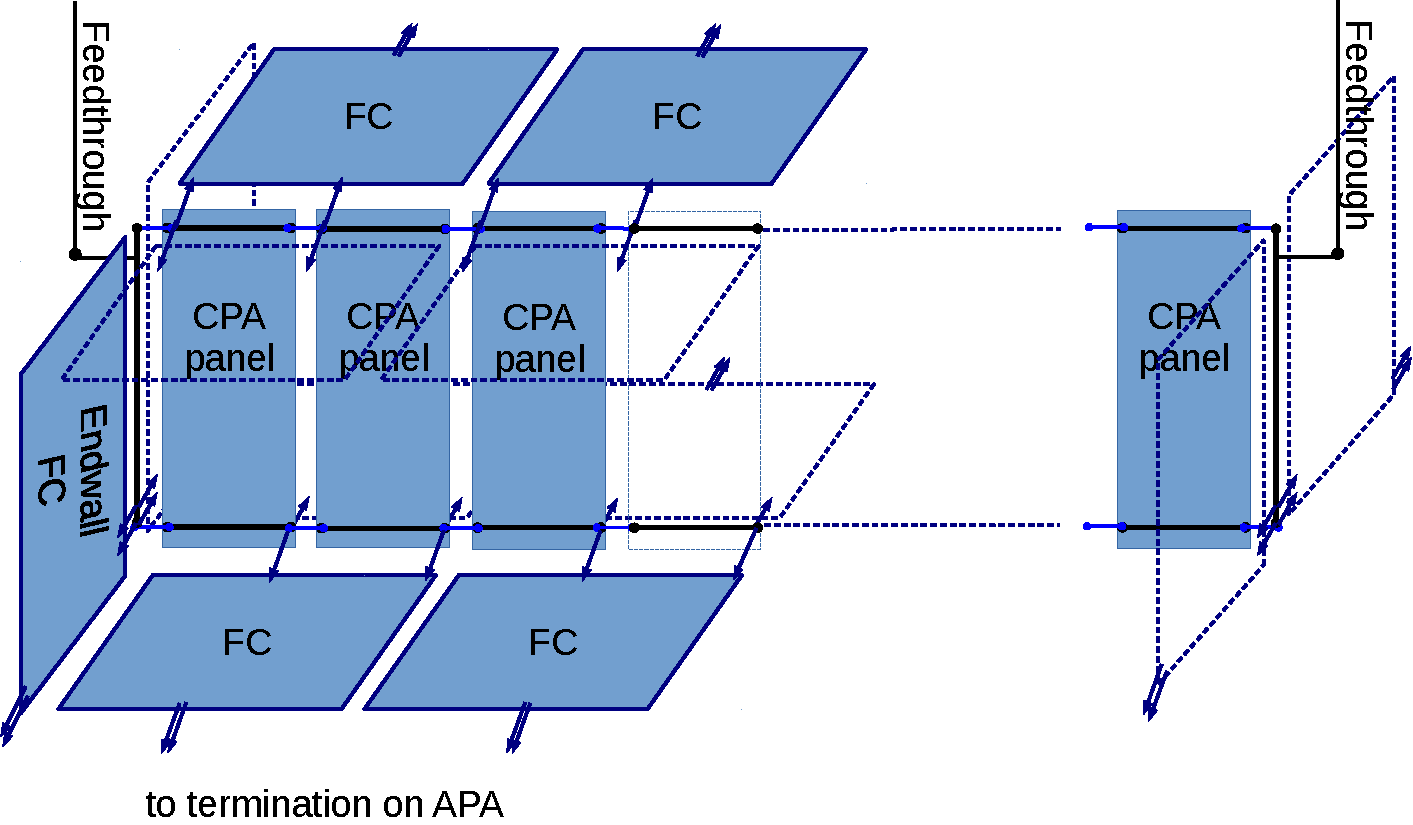
\includegraphics[width=0.7\textwidth]{fdsp-hv-interconnection-topology}
\end{dunefigure}

Electrical interconnections are needed among the \dword{hv} delivery system, \dword{cpa} planes, \dword{fc} modules, and termination
boards on the \dword{apa} modules, as well as between resistive dividers and
the field-forming elements on the \dwords{cpa} and \dwords{fc}.  Redundancy is
needed to avoid single points of failure. 
Some connections must be
insulated in order to avoid creating a discharge path that might
circumvent the discharge mitigation provided by the resistive \dword{cpa}
surface and \dword{fc} partitioning.  Certain connections must be
flexible in order to allow for \dword{fc} deployment, thermal
contraction, and motion between separately supported \dwords{cpa}.  Figure~\ref{fig:fdsp-hv-design-interconnect-concept} shows a high-level
overview of the interconnections between the \dword{hv}, \dword{cpa}, and \dword{fc} modules.


%% connections between major elements (\dword{hv}, \dword{cpa}, \dword{fc}, \dword{apa})
High voltage feedthroughs connect to cups mounted on the \dword{cpa} frame
%\cite the \dword{hv} delivery section
that attach to a \dword{hv} bus running through the \dwords{cpa}.  \Dword{hv} bus connections
between \dword{cpa} panels are made by flexible wires through holes in the
\dword{cpa} frame. The \dword{hv} bus is a loop in order to mitigate risk of a single
point failure; feedthroughs at each end of each \dword{cpa} plane mitigate
risk of a double-break failure.  Voltage dividers on each \dword{cpa} panel
bias the field shaping strips and the resistive dividers on the top
and bottom \dwords{fc}.  \dword{cpa}-to-\dword{fc} connections are made using
flexible wire to accommodate \dword{fc} deployment.  To further
increase redundancy, two \dword{cpa} panels connect to each top or bottom
field cage, and two connections are also made to each \dword{ewfc}. Resistor divider boards attach directly to the interior side of
the \dword{fc} profiles with screws.   A redundant pair of flexible wires
connects a circuit board on the last profile of each \dword{fc} to a
bias-and-monitoring board mounted on the corresponding \dword{apa}.

%% connections within \dword{cpa}
Short sections of flexible wire at the ends of each \dword{hv} bus segment
attach to screws in brass tabs on the \dword{cpa} resistive panels (\dword{cpa} RPs).
%\cite \dword{cpa} design subsection
Vertical \dword{hv} bus segments on the outer ends of each \dword{cpa} plane connect
the top and bottom \dword{hv} buses to complete the loop.  Solid wire is used
to connect resistive panels within a \dword{cpa} panel.

%% \dword{fc} connections
Each \dword{fc} module is as electrically independent as possible in order to
mitigate discharge.  However, only the bottom module of each endwall
can make connections to the \dword{hv} bus and \dword{apa}, so each endwall module
is connected to its upper neighbor at its first and last profiles
using metal strips.

%% Regarding wire terminals and screws
All flexible wires have ring or spade terminals and are secured by
screws in brass tabs.  Spring washers are used with every electrical
screw connection in order to maintain good electrical contact with
motion and changes of temperature.

Table \ref{tab:sp-hv-interconnects} summarizes the interconnections
required.

\begin{dunetable}
[\dword{hv} system interconnections]
{p{0.35\linewidth}p{0.62\linewidth}}
{tab:sp-hv-interconnects}
{\dword{hv} System Interconnections}   
 Connection & Method \\ \toprowrule
 \dword{hv} cup to \dword{hv} bus & wire to screw in \dword{hv} cup mount on \dword{cpa} frame \\ \colhline
 \dword{hv} bus between \dword{cpa} panels & wire between screws in brass tabs \\ \colhline
 \dword{hv} bus to \dword{fss} & wire to circuit board mounted on \dword{fss} \\ \colhline
 \dword{fss} to \dword{topfc} and \dword{botfc} & wire to circuit board on first \dword{fc} profile, two per \dword{fc} module \\ \colhline
 \dword{hv} bus to endwall \dword{fc} & wire to circuit board mounted on first \dword{fc} profile, two per endwall \\ \colhline
 \dword{fc} divider circuit boards & directly attached to profiles using screws and SS slip nuts \\ \colhline
 \dword{fc} to bias and monitoring termination & redundant wires from board mounted on last \dword{fc} profile \\ \colhline
 \dword{hv} bus to \dword{cpa} panels & brass tab on \dword{cpa} resistive panel \\ \colhline
 \dword{cpa} RP interconnections & solid wire between screws in brass tabs \\ \colhline
 Endwall \dword{fc} module interconnections & metal strips, first and last profiles only
 \\ \colhline
\end{dunetable}

The redundancy in electrical connections described above meets requirement (6).
The \dword{hv} bus and interconnections are all made in low field regions in order to meet requirement (2).
The \dword{hv} bus cable is rated at the full cathode \dword{hv} such that even in case of a rapid discharge of the \dword{hv} system no current can flow to the cathode or \dword{fc} except at the intended contact points, preserving the ability of the resistive cathode and \dwords{fc} to meet requirement (5).

%%%%%%%%%%%%%%%%%%%%%%%%%%%%%%%%%%%%%%%%%%%%%%%%%%%%%%%%%%%%%%%%%%%%
\subsection{Interfaces }
\label{sec:fdsp-hv-intfc}

\fixme{ Doc refs must be added to common tdr-citedb.bib - Anne can help with this if you let me know. See format below.  We're also working on the DUNE words; see the all-caps in the table that need fixing.}


\begin{verbatim}
Format for 
@techreport{bib:docdb6754,
title = "{DUNE FD Interface Document: DP CRP to Joint High Voltage}",
author = {{Duchesneau, D. and Pietropaolo, F. and Yu, B.}},
year = {2018},
note = "\url{http://docs.dunescience.org/cgi-bin/ShowDocument?docid=6754&version=1}"
}
\end{verbatim}

\begin{dunetable}
[\dword{hv} system interfaces]
{p{0.25\textwidth}p{0.5\textwidth}l}
{tab:HVinterfaces}
{High Voltage System Interface Links }   
Interfacing System & Description & Linked Reference \\ \toprowrule
\dword{dss}  &  Support, positioning, and alignment of all \dword{cpa}, \dword{fc} modules inside the cryostat both warm and cold & %\citedocdb{nnnn}{n} 
\\ \colhline
\dword{apa} & \dword{fc} support (top, bottom, and end wall) on \dword{apa} frames; Mounting of FC termination filter boards and \dword{fc} failsafe terminations; Mounting of the electron diverter boards. & \citedocdb{6673}{1} 
\\ \colhline
\Dword{ce} & \dword{fc} termination wire connectors on CE feedthrough flange, \Dword{fc} termination wires routed with CE cables & \citedocdb{6739}{4} 
 \\ \colhline
\dword{pds} & Mounting of PD calibration flash diffusers and routing of their fibers to \dwords{cpa}; Possible \dword{tpc} coated reflector foil on \dwords{cpa}. & \citedocdb{6721}{1} 
 \\ \colhline
Facility & Locations and specifications of the \dword{hv} \fdth ports; gas and \dword{lar} flow velocities and patterns. & \citedocdb{6985}{1}  
\\ \colhline
Calibration & \dword{fc} openings for the calibration laser heads & \citedocdb{7066}{1} 
\\ \colhline
\Dword{cisc} & \dword{hv} vs. \dword{lar} level interlock, sensor locations in high field regions, cold/warm camera coverage, \dword{hv} signal monitoring, etc. & \citedocdb{6787}{2} 
 \\ \colhline
\Dword{itf} & Storage buffer, inspections/tests, repackage for underground delivery & \citedocdb{7039}{1} 
 \\ \colhline
Physics & Requirements: range of operating drift field, uniformity of the drift field; Supply detector geometry and \efield{} map. & \citedocdb{7093}{1} 
 \\ 
\end{dunetable}

%%%%%%%%%%%%%%%%%%%%%%%%%%%%%%%%%%%%%%%%%%%%%%%%%%%%%%%%%%%%%%%%%%%%
\section{Production and Assembly }
\label{sec:fdsp-hv-prod-assy}

%%%%%%%%%%%%%%%%%%%%%%%%%%%%
\subsection{Power Supplies and Feedthroughs}
\label{sec:fdsp-hv-supplies-feedthroughs}
Power supplies will be commercially procured, for example through Heinzinger. The \dword{hv} cable is commercially available.

The power supply is tested extensively along with the controls and monitoring software.  Features to be included in the software are:
\begin{itemize}
\item The ability to ramp, or change the voltage.  The rate and an ability to pause the ramp shall be included.  In previous installations, the ramp rate was typically between 60 to 120 V/s.
\item An input for a user-defined current limit.  This parameter is the current value at which the supply reduces the voltage output to stay below the current limit.  The current-limiting is done in hardware.
\item An input for a trip threshold.  At this current reading, the program would reduce the voltage output through software.  In previous experiments, the trip function in software would set the output to \SI{0}{kV}.
\end{itemize}
\noindent Additionally, the software should record the current and voltage read-back values with a user-defined frequency, as well as any irregular current or voltage events.

The \dword{hv} feedthroughs and filters are custom devices.  For fabrication, the feedthrough can be made by collaborators or the design can be sent to a company for completion.  Raw materials such as stainless steel, UHMW PE rods, and flanges are available as stock items and must be machined to make a feedthrough.  Similarly, the resistors, steel or aluminum, and insulator material for the filters can be bought from stock.  The feedthrough and filters shall be tested before being delivered to DUNE.

%%%%%%%%%%%%%%%%%%%%%%%%%%%%
\subsection{Cathode Plane Assembly}
\label{sec:fdsp-hv-prod-cpa}
The component parts of the \dword{cpa} %assembly 
are produced by commercial vendors or university collaborators for the following items:
%\fixme{clearly define cpa vs assembly, mentioned earlier}
\begin{itemize}
\item manufactured FR4 RP frames packed into three \dword{cpa} Unit kits making up a \dword{cpa} Panel,
\item carbon-impregnated Kapton coated resistive panels (RPs) and field shaping strips (\dword{fss}),
\item \dword{hv} cable segments and wire jumpers making up the \dword{cpa} \dword{hv} bus and RP interconnects,
\item resistor boards connecting the RPs to FSS, raising the RP HV by 1.5 kV,
\item machined brass tabs for connecting RPs, \dword{hv} Bus, and \dword{fss}, and
\item top, bottom, and exterior edge profiles and associated connection hardware.
\end{itemize}
The above items are packaged into \dword{cpa} Panel kits and are sent to the assembly factories, the locations of which will be determined later.  The basic construction unit is a pair of \dword{cpa} Panels so that shipment to \surf from an assembly factory consists of two \dword{cpa} Panels that are paired in the underground clean room at \surf to form a \dword{cpa} Plane.

The most basic module of the \dword{cpa} is an RP mounted in a machined slot in the top, bottom and sides of FR4 frames.  There are three different types of these \dword{cpa} RP modules -- an upper, which has as its top frame the \dword{cpa} mounting bracket and \dword{topfc} hinge, a middle, and a lower, which has as its bottom frame a \dword{botfc} hinge.  Two such \dword{cpa} RP modules are bolted together and pinned to form a shipment \dword{cpa} Unit of size \SI{1.2}{\m} $\times$ \SI{4}{\m}.  These \dword{cpa} Units are assembled horizontally on a smooth, flat table to meet the dimensional requirements of \dword{cpa} construction.  In addition to the frames and RPs, %\dword{fss}s 
\dword{fss} strips are mounted on the exposed sides of the FR4 frames, aluminum profiles are attached to the top and bottom of the upper and lower modules, and cables are attached to the RPs to form segments of the \dword{hv} bus.  The shipment \dword{cpa} Unit comes in three varieties in order to make a full \SI{12}{\m} tall \dword{cpa} Panel.  These are : (1) an upper \dword{cpa} RP module attached to a middle module, (2) two middle modules connected, and (3) a middle module attached to a lower module.  The \dword{cpa} Unit order in the shipping crate from top to bottom is middle-and-lower, middle-and-middle, and upper-and-middle.  These 3 \dword{cpa} Units make up one \dword{cpa} Panel.  Two \dword{cpa} Panels are shipped together in one crate - these two Panels will be paired at \surf to form a \dword{cpa} Plane.  For the \SI{10}{\kt} \dword{spmod}, there are 100 upper \dword{cpa} RP modules, 100 lower \dword{cpa} RP modules and 400 middle \dword{cpa} RP modules that make up the 100 \dword{cpa} Panels and 50 \dword{cpa} Planes of the \dword{tpc}.
A comparison of a \SI{6}{\m} \dword{pdsp} \dword{cpa} Panel and a \SI{12}{\m} \dword{pdsp} \dword{cpa} Panel is shown at Ash River Laboratory in Minnesota, USA,  in Figure~\ref{fig:12m-cpa}.

\begin{dunefigure}[\dwords{cpa} at Ash River]{fig:12m-cpa}{A \SI{12}{\m} DUNE-SP \dword{cpa} mockup Panel and a smaller \SI{6}{\m} \dword{pdsp} Panel mockup at Ash River.}  %closest panel 6m, each strip separated by 2m, this image taken in the pit at Ash River (where NOvA modules were stacked/glued.)
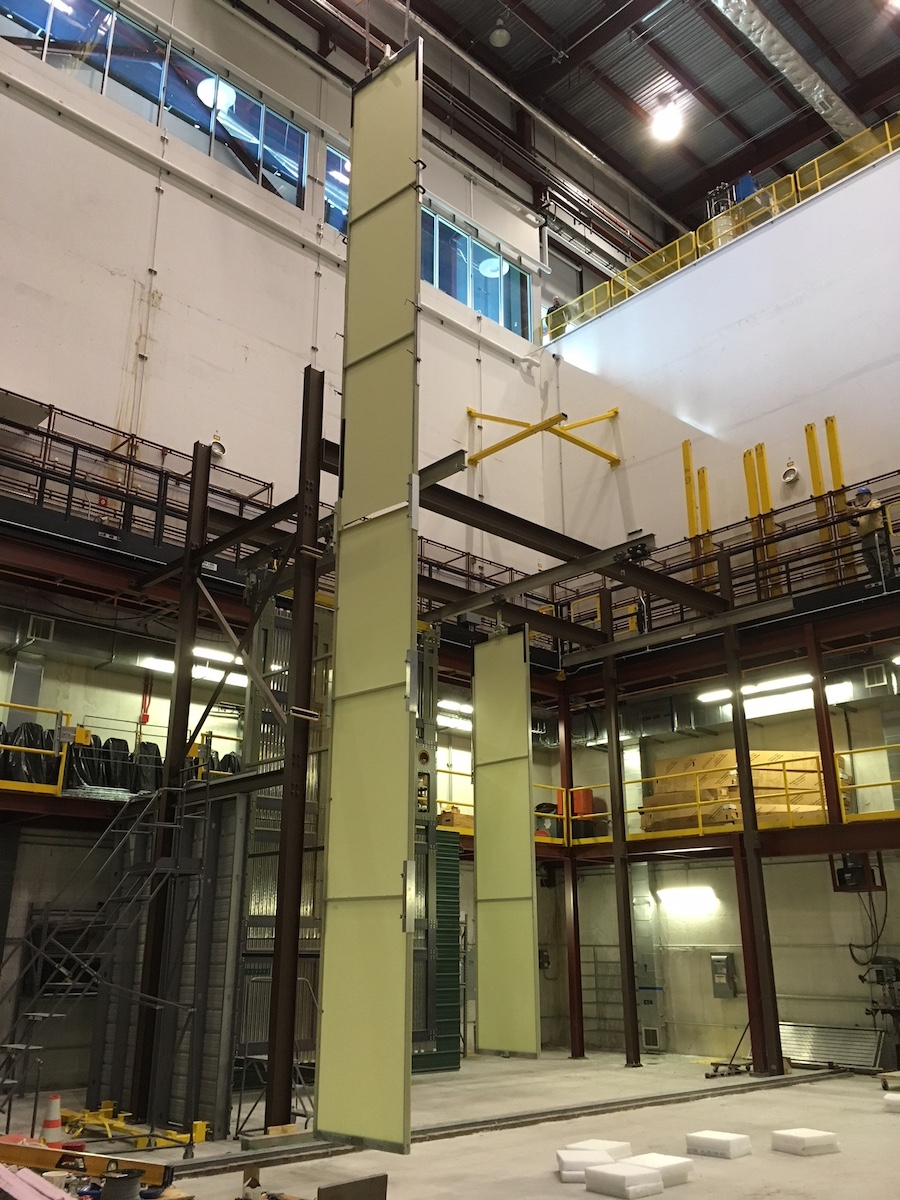
\includegraphics[width=0.5\textwidth]{12m-cpa}
\end{dunefigure}

%%%%%%%%%%%%%%%%%%%%%%%%%%%%
\subsection{Field Cages}
\label{sec:fdsp-hv-prod-fc}

\subsubsection{Top and Bottom Field Cages}

%Discussion of parts procurement, assembly, and testing.
The FRP and FR4 components of the  \dwords{topfc} and \dwords{botfc} will be commercially produced by firms that specialize in the machining of fiberglass components for electrical applications, as was successfully done for \dword{pdsp}. All parts are machined in the absence of water and cleaned with a lacquer thinner. Machined edges, other than small circular holes, are coated with translucent epoxy. The stainless steel and aluminum components will be produced in local university and commercial machine shops. Voltage divider boards and \dword{fc} and \dword{cpa} connection boards will likely be fabricated by university groups.
%The voltage divider boards will be provided by Louisiana State University, and the boards used to make the \dword{fc}/\dword{cpa} connection will be provided by Kansas State University.

The FRP frame assembly primarily consists of fastening together FRP I-beams with FRP threaded rods and hex nuts, which are secured with a limited and specified torque, to avoid damage to the threads. A detailed view of one of these connections is shown in Figure~\ref{fig:tbfc3}.

\begin{dunefigure}[Top and bottom \dword{fc} module frame assembly]{fig:tbfc3}{The above figure shows the procedure for connecting the cross beams to the main I-beams for the \dword{topfc}. Left: The components of each connection, which (from top to bottom) are the threaded rods, the spacer tubes, washer plates, the hexagonal nuts, and an L-shaped FRP brace. An intermediate stage (middle) and final stage (right) of the assembly are also shown."}
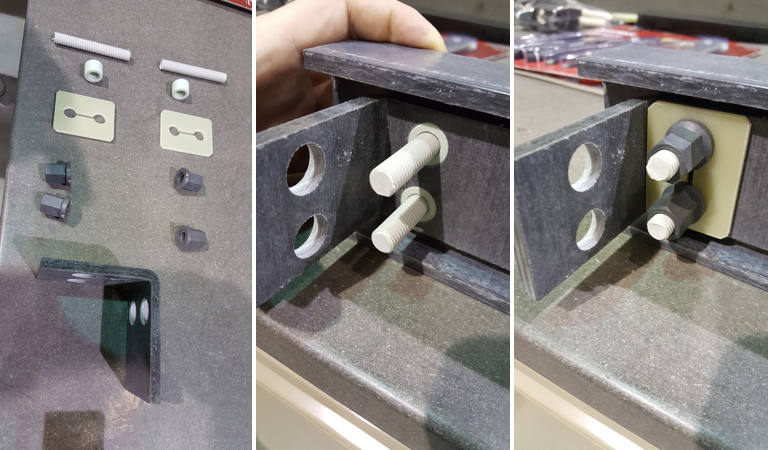
\includegraphics[width=0.70\textwidth]{tbfc3}
\end{dunefigure}

Prior to sliding each profile into the FRP frame, the holes should be covered with Kapton tape to avoid damage to the profile coating. An end cap is attached to each profile using plastic rivets, and then the profiles are aligned against an aligment fixture running the length of the \dword{fc}. After securing each profile to the frame, the tension in the mounting screws is adjusted to remove any angular deflection in the extended portion of the profile.

The ground planes are attached to the 10 cm stand-off I-beam sections with threaded rods and a machined plate. The copper strips are connected to adjacent modules at the same locations. Care must be taken to avoid bending the corners of the \dwords{gp} toward the profiles, particularly on the \dword{cpa} side of of the module.


\subsubsection{Endwall Field Cages}
All FRP plates are commercially cut to shape by water jet. The cut outs in the FRP box beams are also cut by water jet. Holes that accommodate G10 bushings are reamed in a machine shop. FRP frames are pre-assembled to ensure proper alignment of all FRP parts and matching of holes. The profiles are not inserted at this stage. The FRP modules are hung off of each other by means of interconnecting FRP plates to ensure accurate alignment.

Next, parts are labeled and the frames are taken apart. All components are cleaned by pressure washing or ultrasonic bath. All cut FRP surfaces are then coated with polyurethane, which contains the same main ingredient as the FRP resin, allowing it to bond well to the FRP fibers. Final panels are constructed from cleaned and inspected parts. In order to ease assembly, which requires access to both sides of a module,
a dedicated assembly table has been manufactured that allows convenient module rotation. 

Figure~\ref{fig:endwall_assy_rot_table} shows a partially assembled \dword{ewfc} FRP frame on the assembly table.
\begin{dunefigure}[Endwall assembly table]{fig:endwall_assy_rot_table}{Assembly table with partially assembled \dword{ewfc} module (Credit: LSU)}
 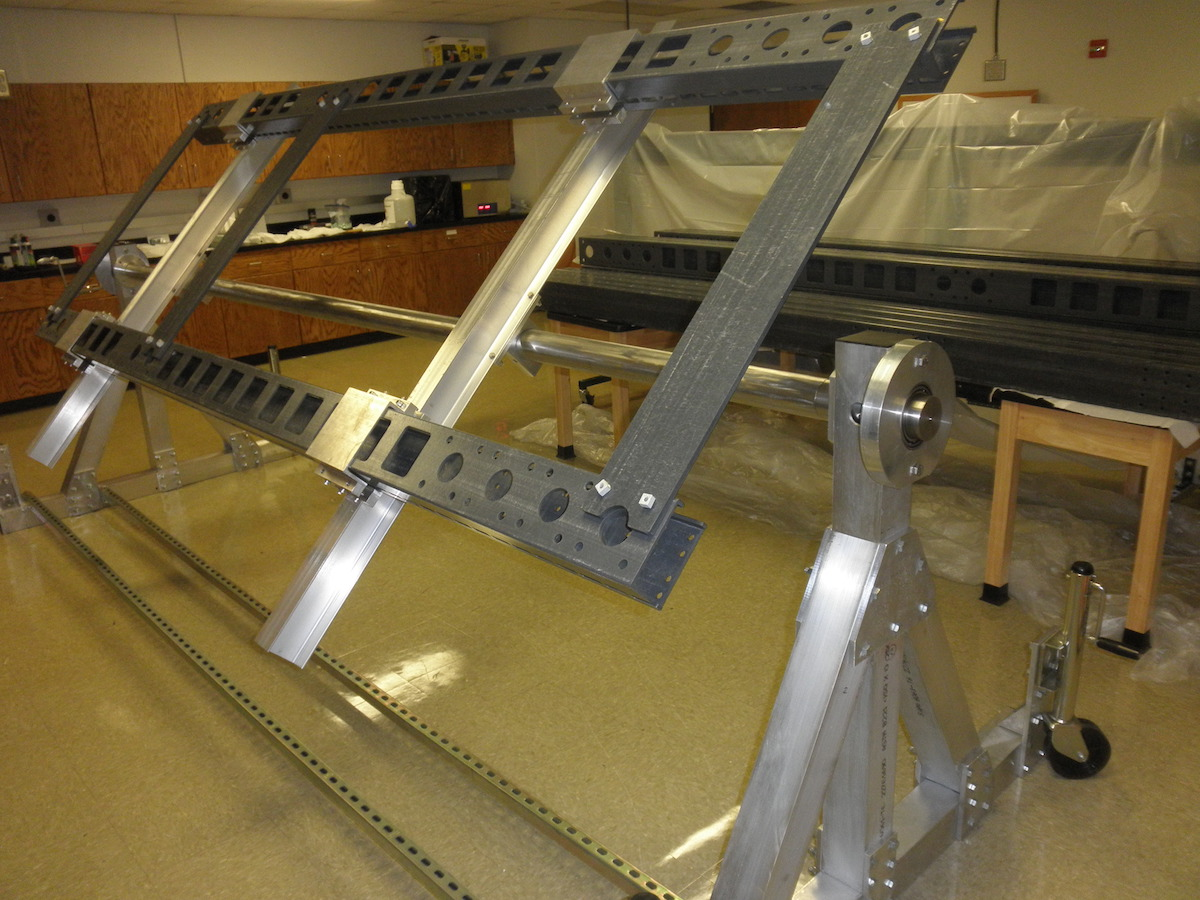
\includegraphics[width=0.8\textwidth]{endwall_assy_rot_table}
 \end{dunefigure}

The FRP box beams are sandwiched between \SI{1.27}{\cm} (\num{0.5}\,in) thick FRP panels which are held on one side by means of G10 bushings and rods with square nuts.
On the other side M10 stainless steel bolts, which are clearly visible in Figure~\ref{fig:endwall_assy_detail},  
engage with large slip nuts that are inserted into the Al profiles. The profiles 
are pulled towards a \SI{2.5}{\cm} thick FRP plate located 
on the inside of the box beam.
%

\begin{dunefigure}[Endwall assembly detail]{fig:endwall_assy_detail}{%Left: Side view of upper part of a top \dword{ewfc}  module.
Top and center \dword{ewfc} module frames hanging. (Credit: LSU)}
%\includegraphics[width=0.48\textwidth]
%{fc_endwall_detail_side}
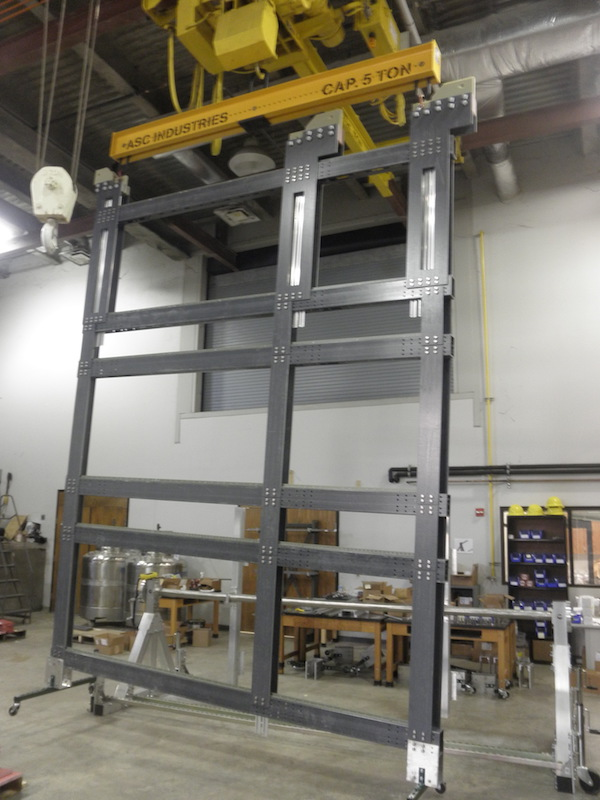
\includegraphics[width=0.5\textwidth]{3_fc_endwall_frames_hanging}
\end{dunefigure}


Aluminum profiles are inserted into the cutouts of the box beams and attached with screws and stainless steel slip nuts to L-shaped FRP brackets that are mounted on the 
FRP box beams. After this, the resistive divider boards are mounted to the profiles using brass screws that engage with stainless steel slip nuts inside 
the profiles.

%%%%%%%%%%%%%%%%%%%%%%%%%%%%
\subsection{Electrical Interconnections}
\label{sec:fdsp-hv-prod-interconnect}

All electrical fasteners and wires used on the \dword{cpa} and \dword{fc} are produced
to specification by commercial vendors and packaged with the \dword{cpa} or \dword{fc} modules.  
As discussed above (\ref{sec:fdsp-hv-prod-cpa}, \ref{sec:fdsp-hv-prod-fc}), 
this includes the \dword{hv} cable segments, as well as wire jumpers, machined brass
tabs, etc.

Circuit boards for %DUNE 
\dword{hv} interconnections are produced and tested at the  university shops according to the same design used for \dword{pdsp}.  The \dword{fc} voltage dividers were produced for \dword{pdsp} at Louisiana State University, and the boards for \dword{cpa} frame bias and \dword{cpa}-\dword{fc} connections were produced at Kansas State University.
%\todo{What about the \dword{fc}-to-\dword{apa} boards?} 
Both institutions have created custom test apparatus for verifying proper operation of the boards at full voltage and over-voltage conditions.  Production and testing could be scaled up by the required order of magnitude at these institutions, or shared with other institutions, whichever best meets the needs of the project. Each board is free of solder flux and flux-remover. 

%%%%%%%%%%%%%%%%%%%%%%%%%%%%
\subsection{Production Safety}
\label{sec:fdsp-hv-prod-safety}

Production of the \dword{fc} panels and resistor-divider boards will involve collaboration technical, scientific, and student labor and  does not present unusual industrial hazards. The \dword{hv} consortium will work closely with each production site to ensure that procedures meet both Fermilab and institutional requirements for safe procedures, personal protective equipment, environmental protection, trained materials handling, and training. The vast majority of production part fabrication will be carried out commercially and shipping will be contracted through approved commercial shipping companies. Prior to approving a site as a production venue, each site will be visited and reviewed by an external safety panel to ensure best practices are in place and maintained. 

\clearpage
%%%%%%%%%%%%%%%%%%%%%%%%%%%%%%%%%%%%%%%%%%%%%%%%%%%%%%%%%%%%%%%%%%%%
\section{Quality Control, Transport, and Installation}
\label{sec:fdsp-hv-transport}
%\fixme{ I added text here and in 1.5.1 for the QA plan and implementation of QC and 1.5.2 for transport and handling - SRM}
A comprehensive Quality Assurance (QA) plan for the production, shipping and installation of the DUNE TPC HV components has been developed based partly on Quality Control (QC) procedures developed and implemented on ProtoDUNE-SP and on successful use of barcode tagging for the NOvA experiment detector elements.  For DUNE, the purity requirements of the liquid argon place restrictions on the introduction of material into the cryostat - so no permanent tags or ink or paint markings on the detector.  A system of temporary tags containing QR or barcodes will be implemented in which the tags are removed when their codes are scanned.  The tag selection requirements are that the tags be large enough and of bright enough color to be seen from both ends of the cryostat.  A particularly cheap and suitable choice is to use bright yellow “cattle tags”.  These are 10-12 square inch plastic tags on which can be printed a unique QR or barcode and can be purchased very cheaply in quantities of hundreds to thousands.
%%%%%%%%%%%%%%%%%%%%%%%%%%%%
\subsection{Quality Control (QC)}
\label{sec:fdsp-hv-transport-QC}
The QC process starts at the production factories by attaching a cattle tag with a unique code to each production unit.  A file linked to each code will contain the individual measurements/properties contained in the QC checklists for that unit.  The following is an example of how this system will be implemented for the CPA:

\begin{itemize}
\item During assembly, QC checklists are filled out electronically using a smart phone or tablet.  Once a 2-module Unit is completely assembled and all checklists have been filled out, a coded temporary cattle tag is attached and scanned, linking the checklist information to the code on the tag.
\item Each 2-module Unit has attached to it a tag with a unique code linking its QC checklists - individual parts for a 2-module Unit are not tagged separately.   A shipping crate will contain six 2-module units each with a removable coded tag plus a hardware package with a coded sticker.
\item A coded label on the shipping crate (paper sticker) will contain contents of crate (6 codes + codes of 2 hardware packages).  This code is only used for shipping purposes and for inventory purposes at the ITF.
\item In the SURF clean room, the 1st CPA Panel is assembled - a coded tag is attached to the CPA Panel and scanned.  The 3 individual Unit tags are then scanned and removed, linking them to the Panel code.
\item The same procedure is followed for the 2nd CPA Panel from crate.  Each panel now has a single tag attached it.
\item The next step is to combine 2 CPA Panels into CPA Plane - a single coded tag is attached to the Plane and scanned.  Then the 2 individual Panel tags are scanned, linking their codes to the that of the Plane.
\item Top/Bottom FC units are attached to both sides of the CPA Plane - a single coded tag on the CPA/FC assembly contains codes of each FC unit (4 tags) and code of the CPA Plane (1 tag) - these 5 tags are removed after scanning.  
\item Moving into the cryostat - the code of the position tag on the DSS is scanned as well as the tag on the CPA/FC assembly - then both tags CPA/FC are removed.
\end{itemize}
At this point, what is obtained is a sequence of linked codes associated with QC checklists that tell which CPA and FC units are mounted in the DSS position with no material left in the cryostat.  A similar sequence is anticipated for the production of the FC Top and Bottom units up to step 6 and separately for the EndWalls.  At the completion of installation in the cryostat and before FC Top and Bottom deployment, visual inspection will confirm the absence of any tags.

%%%%%%%%%%%%%%%%%%%%%%%%%%%%
\subsection{Transport and Handling}
\label{sec:fdsp-hv-transport-transport}
Issues of the means of transportation from HVS production factories to the ITF along with the type of packaging of the shipped units were studied within the HVS Consortium.  The use of cheap, disposable crates to be used between factories and the ITF with transfer to reusable underground crates was compared to the use of just reusable underground crates with return to the factories of empty crates.  It was found that the latter method was cheaper even with the extra shipments of empty crates back to factories.  A vendor was found which produces honeycombed PVC sheets of varying thicknesses which can be formed into crates that can be loaded at the factories, shipped to the ITF, and then sent underground at SURF.  As an example, for the CPA, 50 shipments of crates containing 2 CPA Panels each are required to complete the 10 kt DUNE detector.  With the reusable underground crate scheme in place, only 20 crates are required to make the 50 shipments.  Similar reductions are obtained for the Top and Bottom FC units.  At the start of production, crates would be available at each factory - as shipments are made and installation proceeds at SURF, empty crates are returned to each factory as required.  Inside the crates, individual assembly units are bagged and sealed at the production factory.  At SURF, the crates are lowered into the staging area outside the clean room where the crates are unpacked and the assembly units removed from their bags and taken into the clean room for installation.  The empty crate is then returned to the ITF and then sent back to a production factory for reloading.  Only cleaned assembly units are allowed into the clean room - the crate is restricted to the staging area only.
%%%%%%%%%%%%%%%%%%%%%%%%%%%%
\subsection{Handling Safety}
\label{sec:fdsp-hv-transport-safety}
%\subsection{Assembly and Installation}
%\label{sec:fdsp-hv-install}

\fixme{This section will discuss interaction of HV experts with
Integration team, and reference the appropriate chapter/volume for further details.}
\fixme{Note to editors: It isn't clear to the consortium if the current installation plan requires this section, since ITF handling is conventional. If the section is included, we would like to have the correct phrasing as used by other consortia. -RKP, FP}

%%%%%%%%%%%%%%%%%%%%%%%%%%%%
\subsection{Installation and Integration}
\label{sec:fdsp-hv-transport-install}
%\subsection{Installation and Integration}
%\label{sec:fdsp-hv-integratio}
Installation of the components of the HVS starts with the downstream EndWalls.  The EndWall "toaster" crates containing 4 EndWall modules each are transported into the cryostat.  Two of these crates contain the total of 8 individual modules making up one EndWall between a \dword{cpa} Plane and an APA.  The Endwall modules are removed from their crates starting with the topmost unit and proceeding by attaching subsequent modules until the entire 8 module, 12 m structure is hanging vertically from its support beam.  This is repeated for 3 more assemblies making up the full downstream Endwall - in all, four 8-module assemblies.  

Next, APAs and CPA/FC assemblies are positioned in the order APA, CPA/FC, APA, CPA/FC, and APA making up the first row of 25 in the detector.  Electrical and mechanical connections between the EndWalls and APAs and the Endwalls and \dword{cpa} Arrays are made.  At this point, deployment of the Top and Bottom FC units attached to the \dword{cpa} Planes is done.  Once the Top and Bottom FCs are latched at the APA ends, the TPC row is complete.  Subsequent rows of APAs and CPA/FC assemblies are positioned in order, completing 25 rows of the TPC volume.  Once the 25th row is in place, the Top FC units are deployed, latching to the APAs.  Before the Bottom FCs are deployed, the upstream EndWall crates are brought into the cryostat and the Endwalls are built up from their crates in the same manner as the downstream Endwalls - four 8-module Endwall assemblies between APAs and \dword{cpa} Planes.  Once the Endwalls are in place, the Bottom FCs are deployed, finishing the TPC field cage volume of the detector.  Finally, electrical and mechanical connections between EndWalls and APAs and between Endwalls and \dword{cpa} Arrays are made completing all field cage connections in the TPC.

%\fixme{This is the order so far - SRM}

\begin{dunefigure}[\Dword{pdsp} \dword{cpa} plane before and after \dword{fc} attachment]{fig:cpas-in-cryostat}{Left: Completed \dword{pdsp} \dword{cpa} plane ready for \dword{fc} attachment. Right: Two completed \dword{cpa}-\dword{fc} assemblies in the \dword{pdsp} cryostat. The top and bottom \dwords{fc} with their \dwords{gp} attached are visible to the right of the cathode plane in their folded-up pre-installation position.}
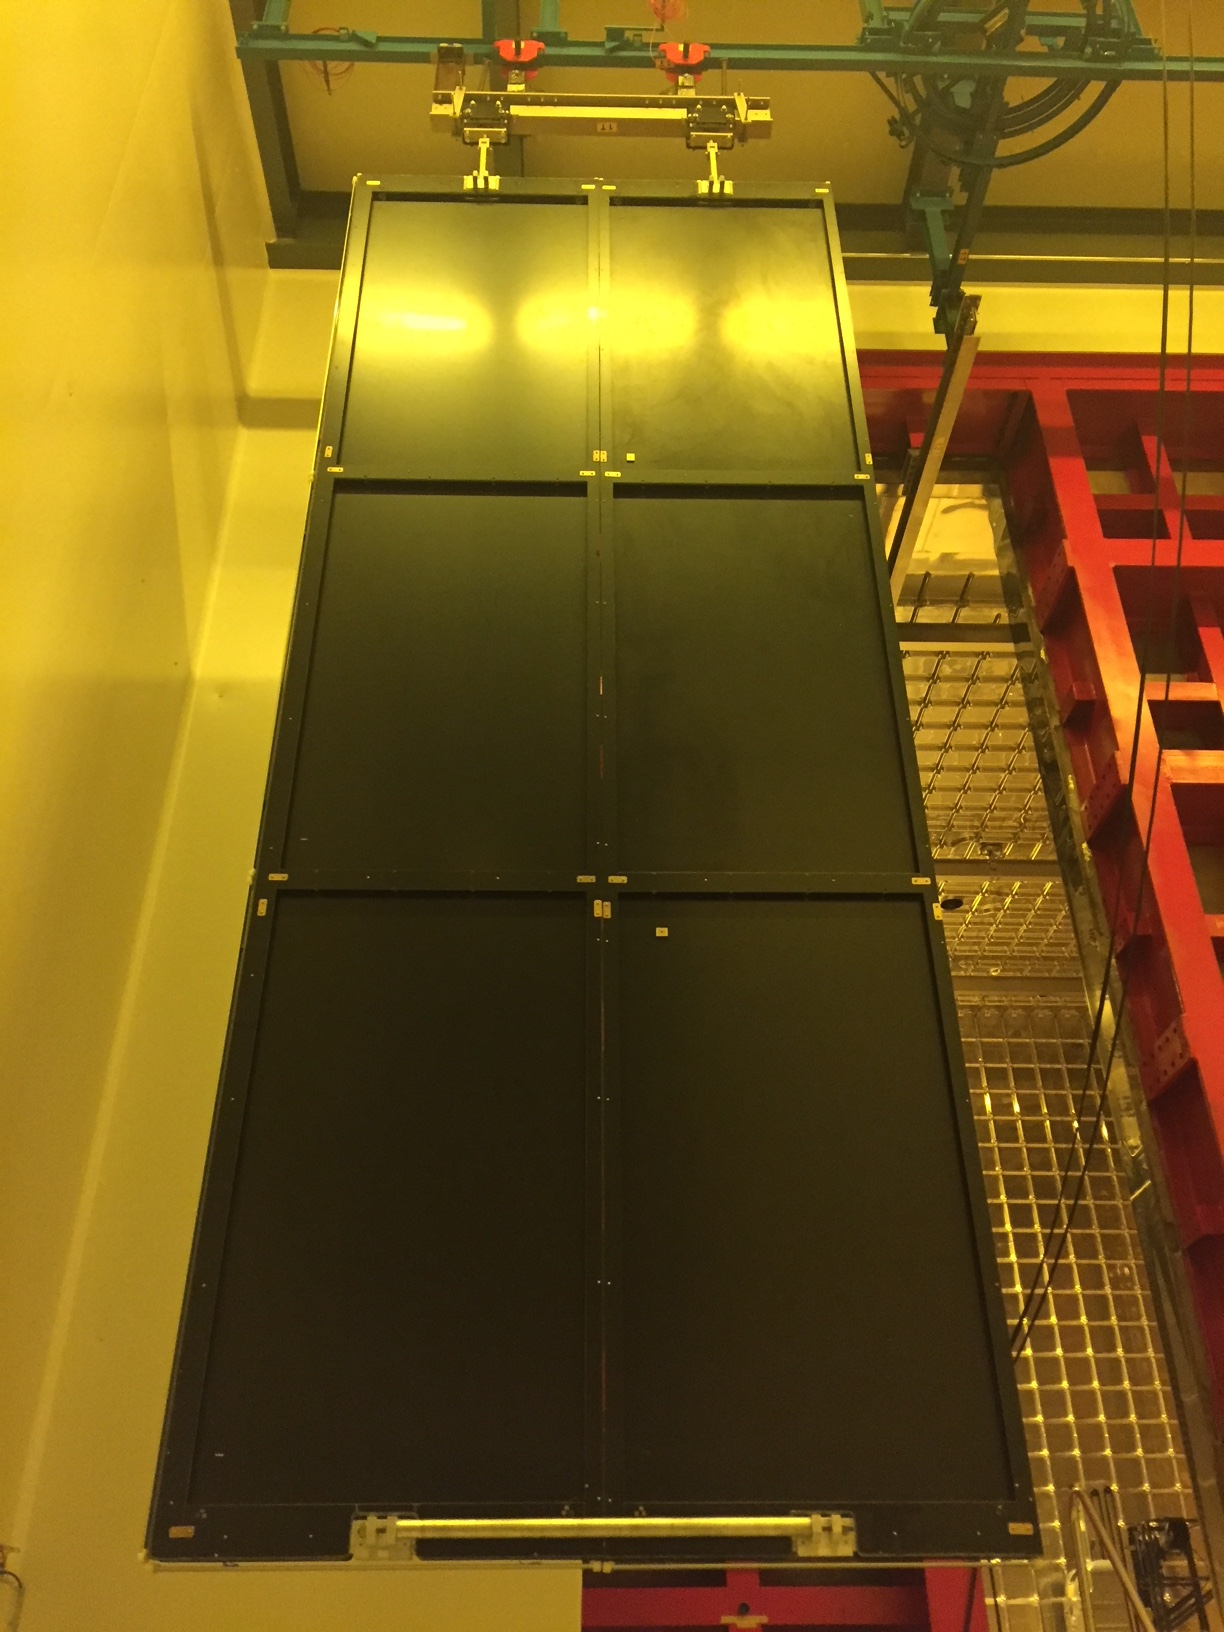
\includegraphics[width=0.45\textwidth]{lastcpa}
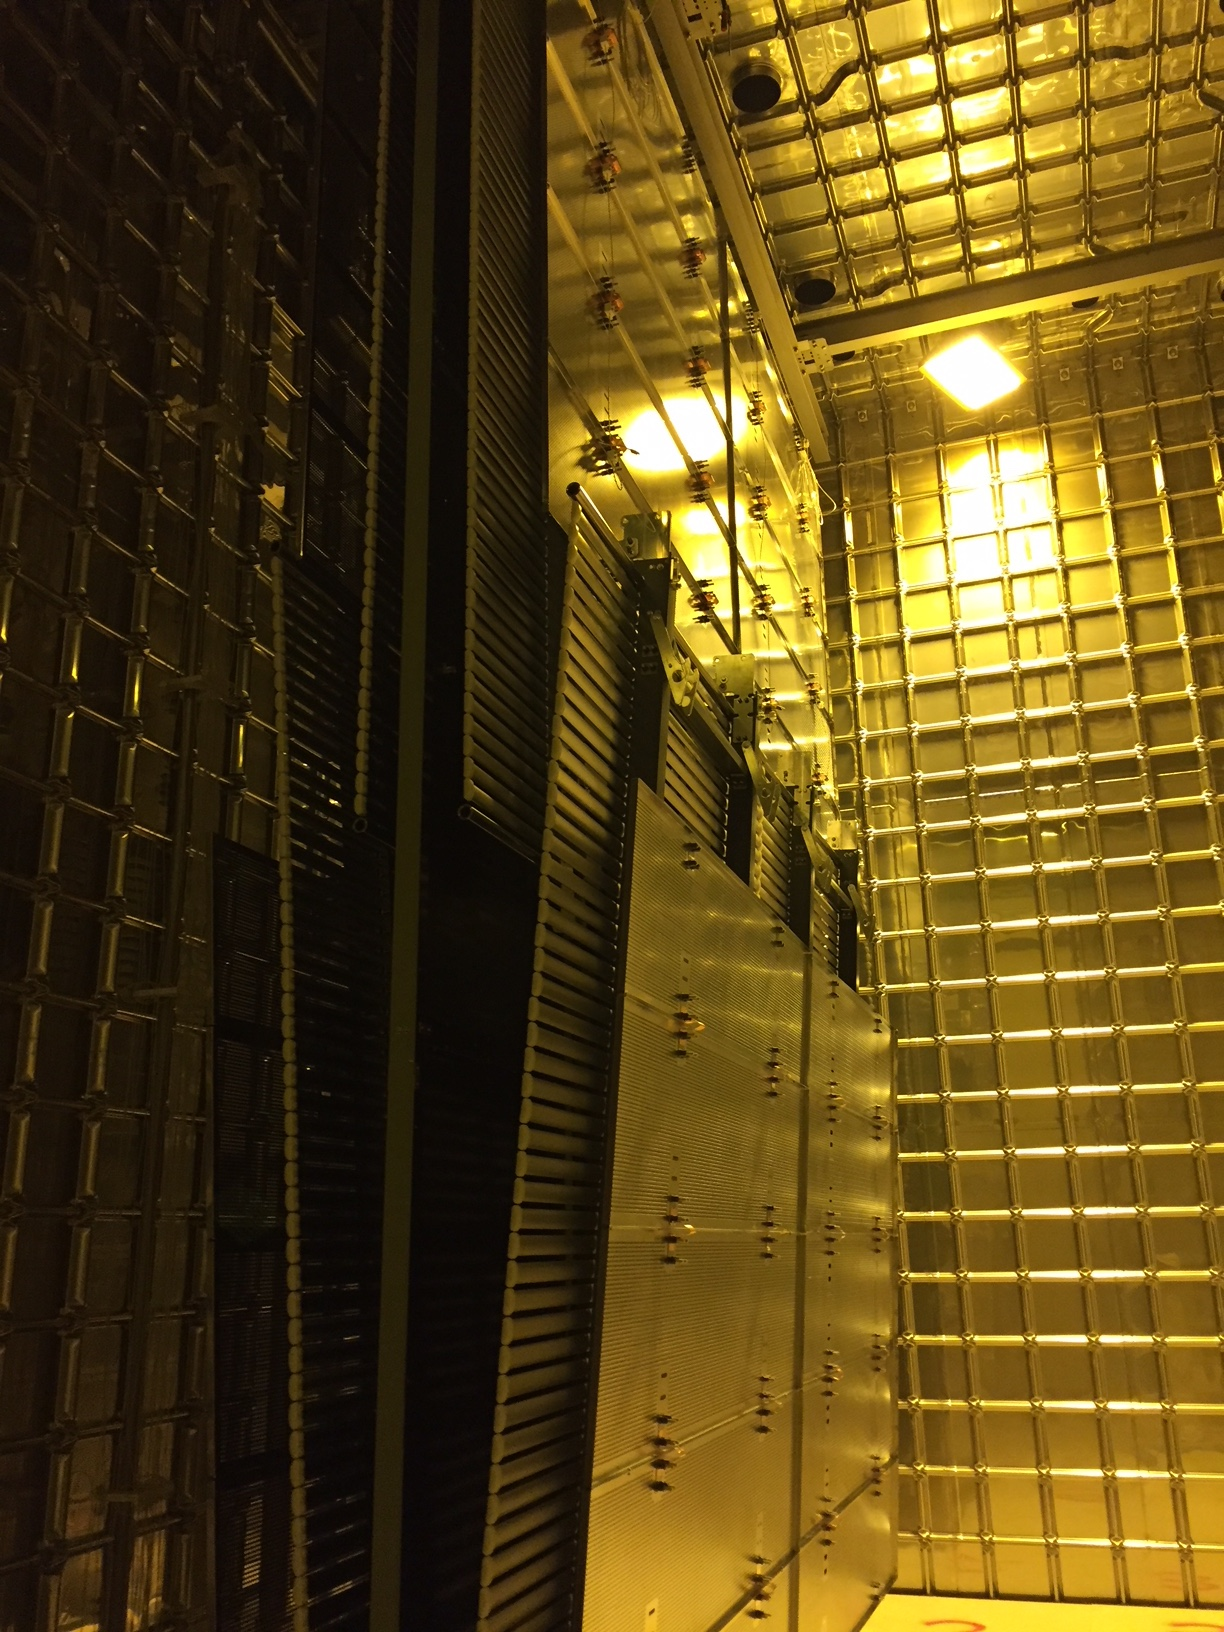
\includegraphics[width=0.45\textwidth]{2cpas-in-cryostat}
\end{dunefigure}

\begin{dunefigure}[\Dword{pdsp} \dword{ewfc} installation]{fig:EndwallInstall}{Completed endwall in process of installation into \dword{pdsp} cryostat.}
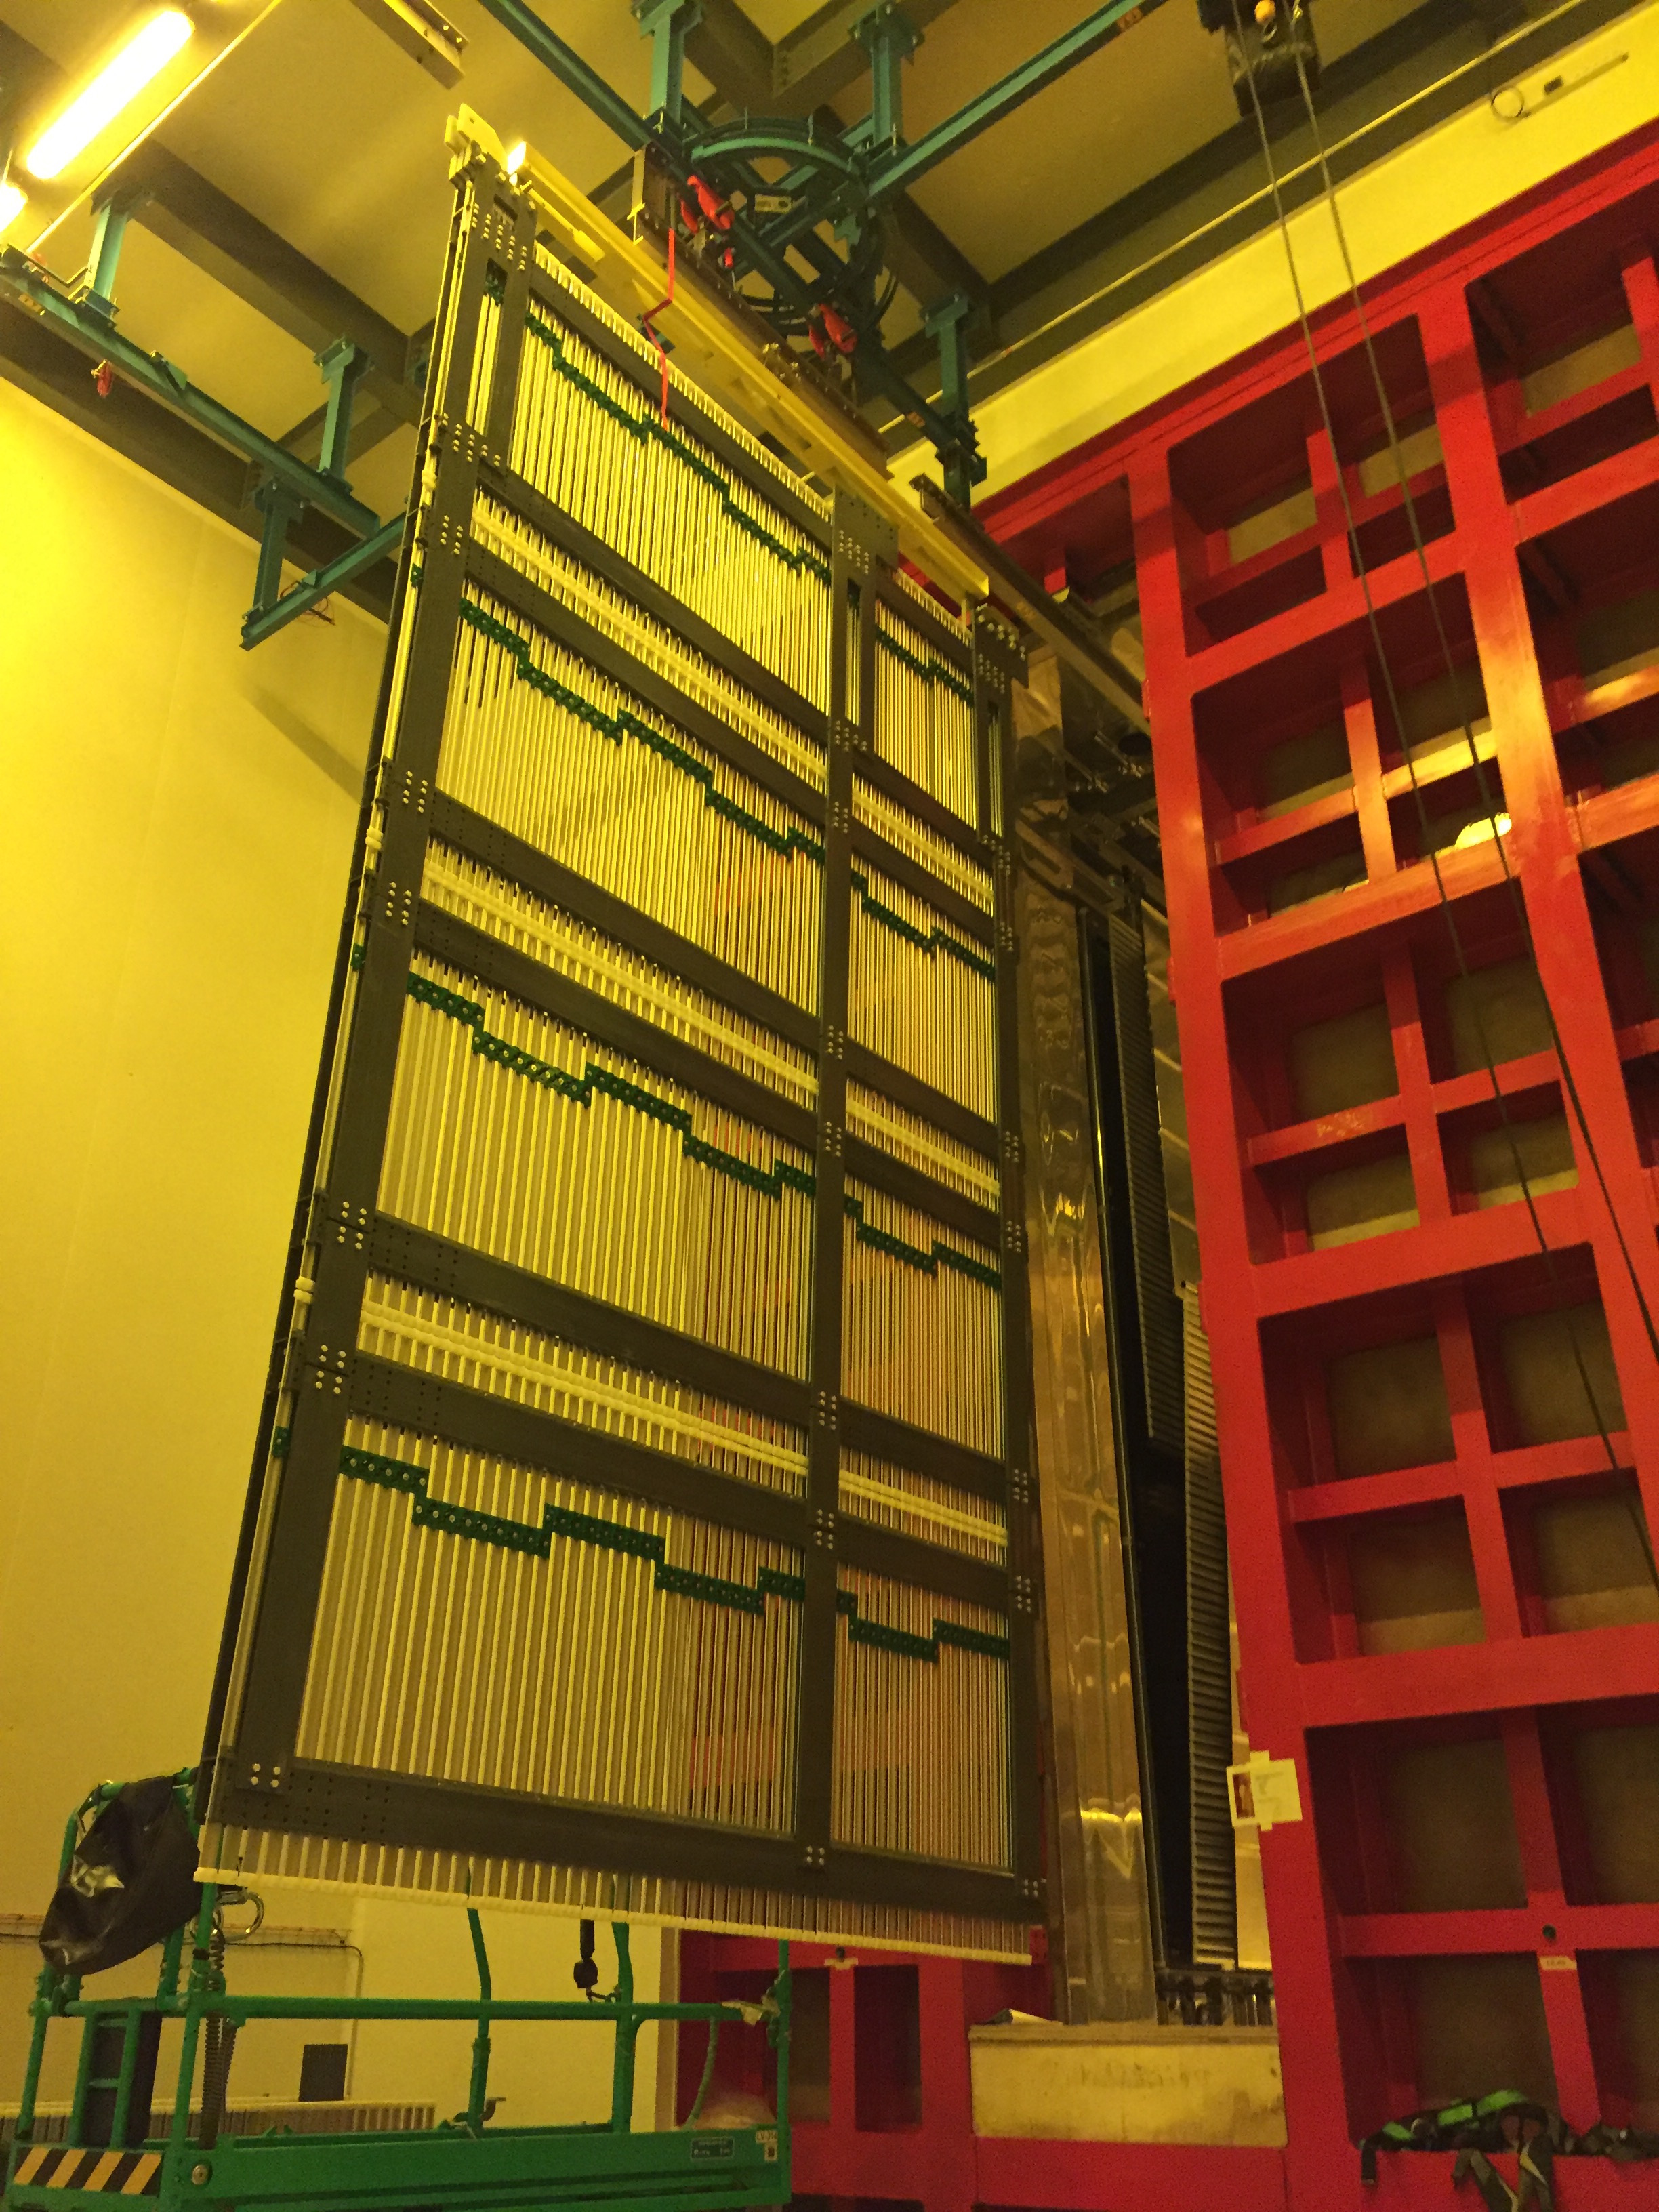
\includegraphics[width=0.45\textwidth]{endwall_and_tco.jpg}
\end{dunefigure}


\clearpage
%%%%%%%%%%%%%%%%%%%%%%%%%%%%%%%%%%%%%%%%%%%%%%%%%%%%%%%%%%%%%%%%%%%%
%\section{Quality Control (QC)}
%\label{sec:fdsp-hv-qc}
%\clearpage
%%%%%%%%%%%%%%%%%%%%%%%%%%%%%%%%%%%%%%%%%%%%%%%%%%%%%%%%%%%%%%%%%%%%
%\section{Safety}
%\label{sec:fdsp-hv-safety}
%\clearpage
%%%%%%%%%%%%%%%%%%%%%%%%%%%%%%%%%%%%%%%%%%%%%%%%%%%%%%%%%%%%%%%%%%%%
\section{Organization and Management}
\label{sec:fdsp-hv-org}

%%%%%%%%%%%%%%%%%%%%%%%%%%%%

\subsection{Institutional Responsibilities}
\label{sec:fdsp-hv-org-consortium}
The consortium has consolidated all the institutions that have participated in the design, construction and assembly of the \dword{hv} systems for both \dword{pdsp}  and \dword{pddp}. 

The consortium is currently composed of US institutions and CERN, presently the only non-USA participant. As in the case of \dword{protodune}, CERN is heavily committed to a significant role in terms of funding, personnel, 
 and the provision of infrastructure for R\&D and detector optimization. Moreover, CERN will be responsible for a significant fraction of subsystem deliverables; as such  CERN is actively in search of additional European institutions to attract into the consortium. 
 
 The present consortium organization structure includes a leader (currently from CERN), a technical lead (currently from BNL), a \dword{tdr} editor (currently from \fnal), and a HVS design and integration lead (currently from ANL). 

In the \dword{hv} consortium organization, each institution is naturally assuming the same responsibilities as for the developments of \dword{pdsp}. The consortium is organized into working groups addressing the design and  R\&D phases and the hardware production and installation.

\begin{itemize}
\item WG1. Design optimization for \dword{spmod} and \dword{dpmod}; assembly, system integration, detector simulation, physics requirements for monitoring and calibrations. %Conveners: Jeff Nelson, Vic Guarino, Bo Yu
\item WG2. R\&D activities, R\&D facilities. %Conveners: Francesco Pietropaolo, Ting Miao
\item WG3. \dword{sp}-\dword{cpa}: Procurement, in situ \dword{qc}, resistive panels, frame strips, electrical connections of planes; \dword{qc}, assembly, shipment to assembly site; \dword{qc}. %Convener: Stephen Magill
\item WG4. \dword{dp} cathode.% Convener: Jae Yu
\item WG5. \dword{fc} modules. %Conveners: Thomas Kutter, Michael Wilking, Jeff Nelson, Jae Yu
\item WG6. \dword{hv} supply and filtering, \dword{hv} power supply and cable procurement, R\&D tests, filtering and receptacle design and tests. %Conveners: Franco Sergiampietri, Sarah Lockwitz
\end{itemize}

\noindent Merging of \dword{sp} and \dword{dp} activities is performed for the working groups where synergies have been identified: \dword{hv} feedthroughs, voltage dividers, aluminum profiles, FRP beams, and assembly infrastructure.

\begin{dunetable}
[Participating intitutes]
{p{0.15\textwidth}p{0.75\textwidth}}
{tab:instit}
{Institutes participating in the HVS consortium}   
ID & Institution (Contact, E-mail) \\ \toprowrule

1 & CERN, Switzerland (Francesco Pietropaolo; francesco.pietropaolo@cern.ch) \\ \colhline
2 & Argonne National Lab, USA (Steve Magill; srm@anl.gov) \\ \colhline
3 & Brookhaven National Lab, USA (Bo Yu; yubo@bnl.gov) \\ \colhline
4 & University of California Berkley / LBNL, USA (Cheng Ju Lin; cjslin@lbl.gov) \\ \colhline
5 & University of California Davis, USA (Emilja Pantic; pantic@ucdevis.edu) \\ \colhline
6 & Fermi National Accleratior Lab, USA (Sarah Lockwitz; lockwitz@fnal.gov) \\ \colhline
7 & University of Huston, USA (Andrew Renshaw; arenshaw@central.uh.edu) \\ \colhline
8 & Kansas State University, USA (Glenn Horton-Smith; gahs@ksu.edu) \\ \colhline
9 & Louisiana State University, USA (Thomas Kutter; kutter@phys.lsu.edu) \\ \colhline
%10 & South Dakota School of Mines and technology, USA (Juergen Reichenbacher; Juergen.Reichenbacher@sdsmt.edu) \\ \colhline
10 & SUNY Stony Brook, USA (Michael Wilking; michael.wilking@stonybrook.edu) \\ \colhline
11 & University of Texas Arlington, USA (Jaehoon Yu; jaehoonuy1@gmail.com) \\ \colhline
12 & Virginia Tech, USA (Jon Link; jmlink@vt.edu) \\ \colhline
14 & College of William and Mery, USA (Jeff Nelson; jknels@wm.edu)  \\ 
\end{dunetable}




%%%%%%%%%%%%%%%%%%%%%%%%%%%%
\subsection{Risks}
\label{sec:fdsp-hv-org-risk}

%\fixme{Some text must accompany the table. The "ID" in the table refers to the ID in the Risk Register.}
Most of the items presented in the Risk Table are the same in \dword{pdsp} and the \dword{dune} \dword{sp} and have been addressed with \dword{pdsp} (except ID's 10, 11 and 14 that are specific of the Far Detector Underground Installation). None of these items have caused significant problems during the commissioning and early operation of \dword{pdsp}, with the partial exception of  ID 6: current streams, localized on one specific FC module and occuring at intervals of several hours, required a few minutes ramp-down of the HV from the nominal 180 kV to a lower value, typically 140-160 kV (please see section \ref{sec:fdsp-hv-protodune}). Investigations are underway to characterize and mitigate this risk.
ID 5 requires an accurate analysis of collected muon data, (This is a work-in-progress activity.) and the disentangling of space charge effects. 
These risks still persist for the far detector case, given the much larger detector scale and the more complex underground installation environment.

\begin{dunetable}
[High Voltage System Risk Summary]
{p{0.15\textwidth}p{0.75\textwidth}}
{tab:HVrisks}
{High Voltage System Risk Summary}   
ID & Risk \\ \toprowrule

1 & Broken resistors on voltage divider boards \\ \colhline
2 & Broken varistors on voltage divider board \\ \colhline
3 & CPA: scratches on double coated resistive panels\\ \colhline
4 & CPA: scratches on  resistive strips on the frame \\ \colhline
5 & Electric field uniformity is not adequate for muon momentum reconstruction \\ \colhline
6 & Electric field is below specification during stable operations\\ \colhline
7 & Damage to CE in event of discharge \\ \colhline
8 & Detector components are damaged during shipment to the far site  \\ \colhline
9 & Damages (scratches, bending) to aluminum profiles of Field Cage modules  \\ \colhline
10 & International funding level for SP HVC too low  \\ \colhline
11 & Sole source for Kapton resistive surface; and may go out of production \\ \colhline
12 & Free hanging frames can swing in the fluid flow  \\ \colhline
13 & FPR/Polyethene/laminated Kapton component lifetime is less than expected  \\ \colhline
14 & Underground installation is more labor intensive or slower than expected  \\ 
\end{dunetable}

%%%%%%%%%%%%%%%%%%%%%%%%%%%%
\subsection{High-level Cost and Schedule}
\label{sec:fdsp-hv-org-cs}

%\fixme{Some text must accompany the tables.}

A first high-level summary of the material cost estimate for the \dword{hv} system of one \dword{spmod} has been obtained extrapolating from the as-realized \dword{pdsp} costs and and effort. No costs for spare parts has been included, and no contingency. On the other hand, these estimates also do not include any projected cost savings that will be realized by producing many units at each production site. Given the small numbers of each unit required for the \dword{pdsp} (e.g., 12 \dword{topfc} and \dword{botfc} modules and 16 \dword{ewfc} modules) the assembly sites were still climbing the learning curve; this could give additional substantial savings. 

A tentative schedule of the HVS system for the first Single Phase Far Detector is given. It includes the most relevant short term milestones. Dates are calculated assuming the the Start of installation at SURF given in the last line of the table.

%\begin{dunetable}
%[\dword{hv} system materials costs]
%end{dunetable}
\begin{dunetable}
[High Voltage System Cost Summary]
{p{0.7\textwidth}p{0.2\textwidth}}
{tab:HVcostsumm}
{High Voltage System Cost Summary}   
Item & Core Cost (k\$ US) \\ \toprowrule

Design, Engineering, and R\&D & \num{243.3} \\ \colhline
Physics \& Simulations & \num{20.0} \\ \colhline
CPA Production Setup & \num{37.0} \\ \colhline
T/B FC Production Setup & \num{37.0} \\ \colhline
EW FC Production Setup & \num{44.0} \\ \colhline
HV feedthrough cold test setup & \num{5.0} \\ \colhline
CPA Production  & \num{3630.4} \\ \colhline
FC common components production  & \num{1808.1} \\ \colhline
Top/Bottom FC module production & \num{938.1} \\ \colhline
End wall FC module production & \num{757.2} \\ \colhline
HV Components Production & \num{269.0} \\ \colhline
Shipping \& Integration  & \num{35.7} \\ \colhline
Installation & \num{47.7} \\ \colhline \colhline
Total SP HV System (SP-HV) & \num{7867.4} \\
\end{dunetable}





\begin{dunetable}
[High Voltage System Schedule]
{p{0.65\textwidth}p{0.25\textwidth}}
{tab:HVsched}
{High Voltage System Schedule and Milestones}
Milestone & Date (Month YYYY) \\ \toprowrule
CPA/FC/EndWall Design Review (60\%)  & February 2019 \\ \colhline
CPA/FC/EndWall Mod 0 (for tests at Ash River) & June 2019  \\ \colhline
CPA/FC/EndWall Production Readiness Review    & August 2020   \\ \colhline
Start Procurement for  CPA  & January 2020   \\ \colhline
CPA factory set-up  & July 2022 \\ \colhline
Start CPA production  & September 2022 \\ \colhline
Field Cage Profiles Order   & January 2022 \\ \colhline
Start Procurement of T/B Field Cage Parts & February 2022 \\ \colhline
T/B FC factory set-up  & July 2022 \\ \colhline
Start T/B FC production  & September 2022 \\ \colhline
Start Procurement of E-W Field Cage Parts & September  2020 \\ \colhline
E-W FC factory set-up  & March 2022 \\ \colhline
Start E-W FC production  & July 2022 \\ \colhline
Start of installation at SURF     & May 2023 \\
\end{dunetable}



\clearpage

%%%%%%%%%%%%%%%%%%%%%%%%%%%%%%%%%%%%%%%%%%%%%%%%%%%%%%%%%%%%%%%%%%%%

\section{Appendix - Alternatives}

\subsection{Optical Reflectors on \dword{cpa}}

Since the \dword{pd}s in the current \dword{tpc} design are installed only on the \dword{apa} side of the drift volume and have low coverage, their responses to ionization inside the \dword{tpc} are highly drift distance dependent and severely biased toward the \dword{apa}.  In order to improve the uniformity of response along the drift direction, the \dword{pd} has proposed to add WLS coated reflector foils to convert the UV photons arriving at the cathode into visible photons and bounce them back to the \dword{pd}s inside the \dword{apa}s.  Simulations have shown that the addition of the reflectors makes a  significant improvement in the uniformity of response.

Implementing this concept, however, could dramatically alter the current \dword{cpa} characteristics and design.  Several concepts have been developed by the HVS to accommodate the reflectors with minimal change to the current \dword{cpa} design.  The main issue here is the conductivity of the reflector foil vs. the highly resistive nature of the \dword{cpa}s.  One would like to cover as much of the cathode surfaces as possible to improve the light output.  However, if the reflectors are conductive, aluminum coated for example, large area coverage with these reflectors could short circuit the resistive cathode and render it ineffective in slowing down the energy transfer during a HV breakdown.  On the other hand, if the reflector foils are insulators, they would intercept the ionization drifting toward the cathode and become charged.  This would alter the drift field uniformity, and worst yet, possibly result in random breakdowns through the foil.

A design concept that is fairly simple to implement and using known material is depicted in Fig.\ref{fig:reflectorOnCPA}.  A 3M Vikuiti reflector foil is laminated on a thin FR4 backing sheet to maintain CTE compatibility with the resistive \dword{cpa} panel which also has an FR4 core. The reflector foil assembly is perforated at regular intervals to allow electrons to be collected through the holes to the CPA surface, minimizing the voltage build up from charging of the non-perforated surfaces.  Several such foil assemblies are then tiled on the existing CPA resistive panels with screws.

In order to advance the \dword{cpa} design while providing the option of adding the reflector foils at a later time, the HVS will design in a set of hole pattern on the \dword{cpa} resistive panels, which could be used for mounting of reflector foils/panels, or left unused without negative consequences. In the meantime, HVS and PDS are conducting joint R\&D to evaluate a few design concepts and material choices. 

\begin{dunefigure}[Reflector on \dword{cpa} concept]{fig:reflectorOnCPA}{A concept to attach reflector foils to a \dword{cpa}. (Credit: BNL)}
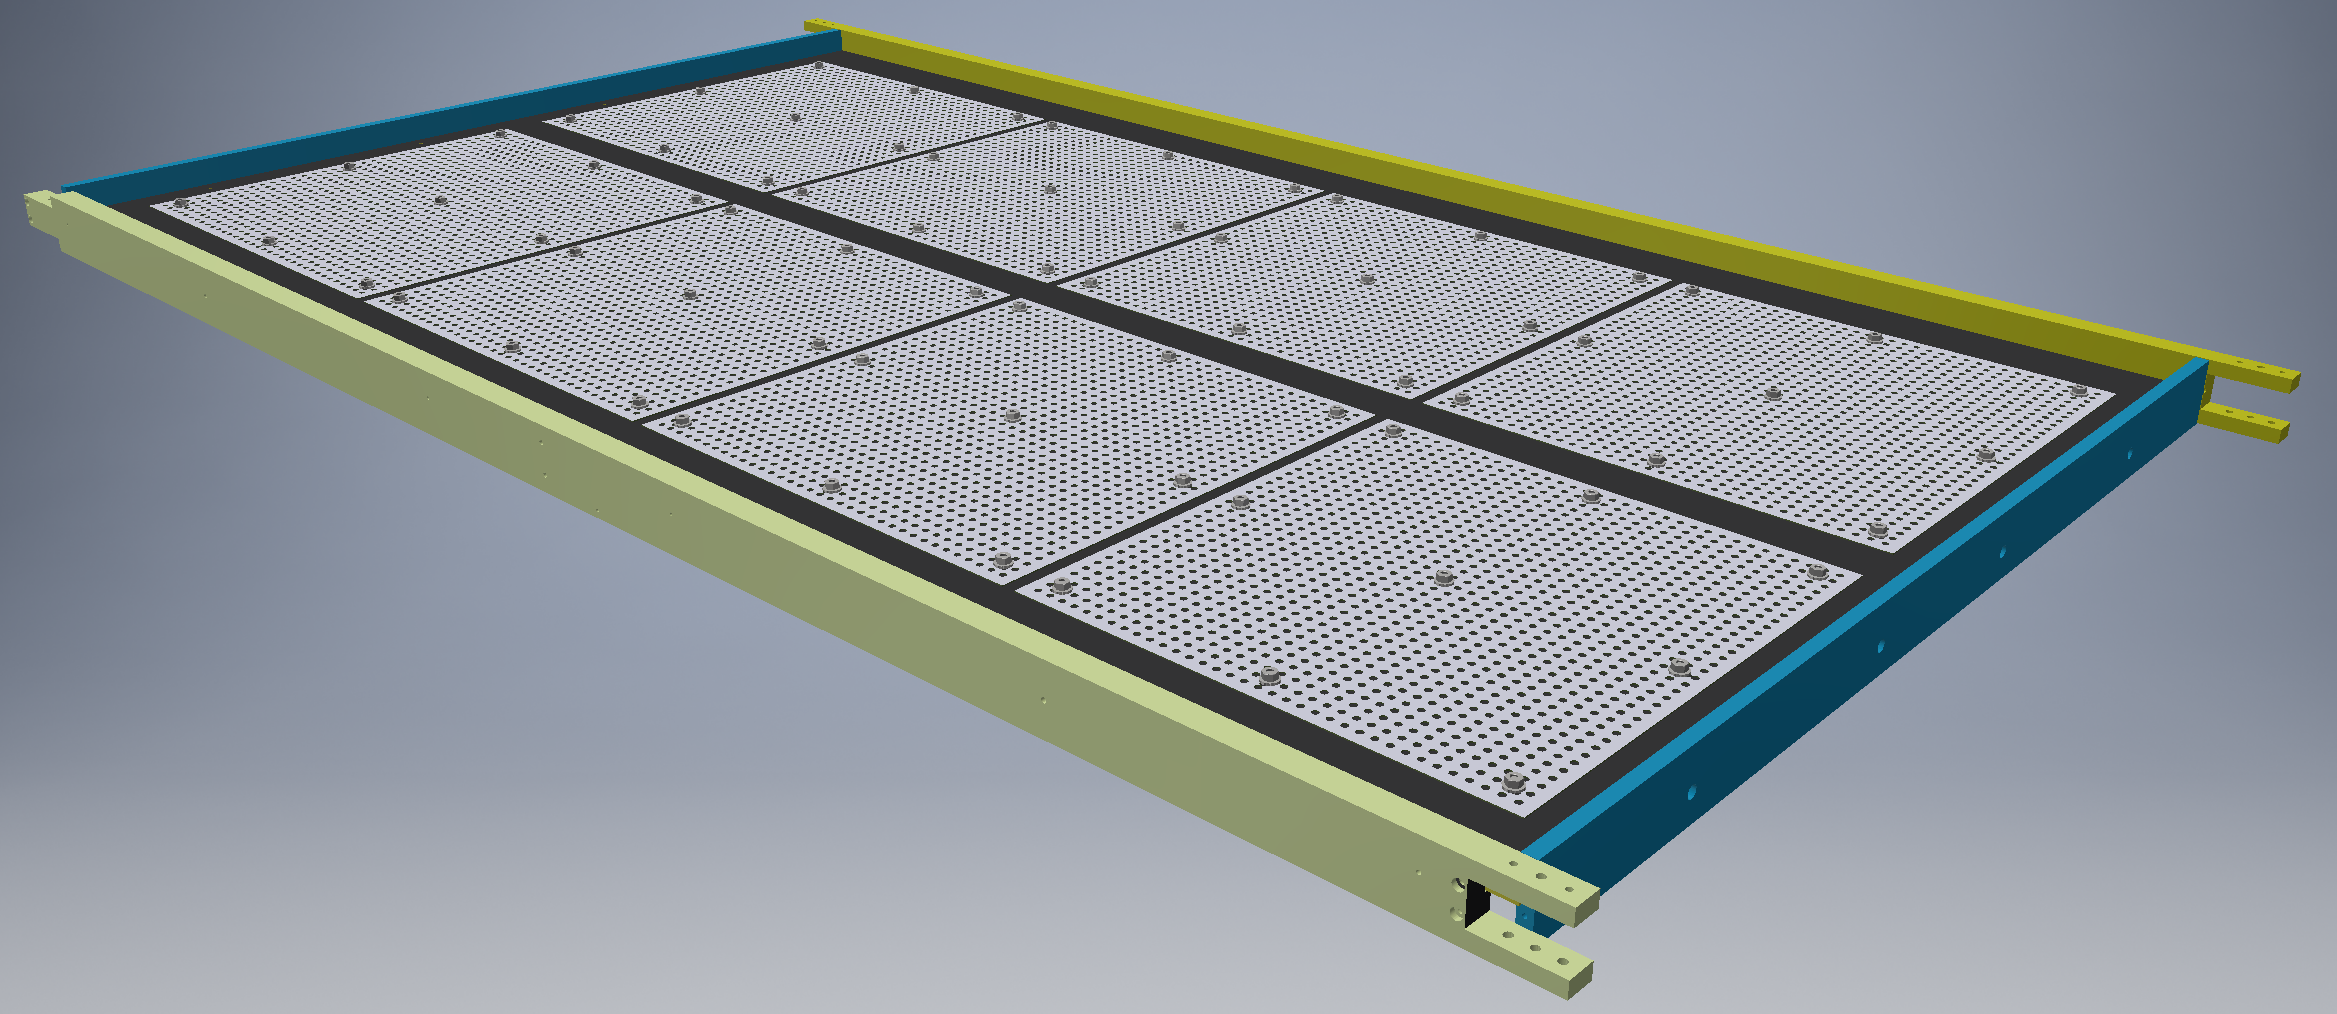
\includegraphics[width=0.9\textwidth]{ReflectorOnCPA.png}
\end{dunefigure}

\subsection{Calibration Laser Penetrations}

The Calibration Consortium is developing requirements for calibrating the \dword{tpc} electric field.  One existing technique is to use UV laser beams to ionize the \dword{lar} and generating straight tracks along known trajectories.  Since the field cage surrounds the \dword{tpc} active volume, one needs to either shoot through the gaps between the field cage profiles (as in MicroBooNE), or make openings in the field cage for the laser heads to pass through (as in SBND).    Fig.\ref{fig:SBND_laser}  shows the design of a corner of the SBND \dword{tpc} with a field cage opening, and a calibration laser head through the opening.  Implementing such openings is straightforward, if the openings are at the field cage module boundaries.  Doing so through the interior surface of a field cage panel is more complicated, but still simpler than the beam plug we designed for the ProtoDUNE SP.  There will be some minor drift field distortion around the openings.  Preliminary FEAs have shown the field distortion to be negligible. 

\begin{dunefigure}[SBND laser arrangement]{fig:SBND_laser}{SBND field cage opening to allow a calibration laser head to pass through. (Credit: BNL)}
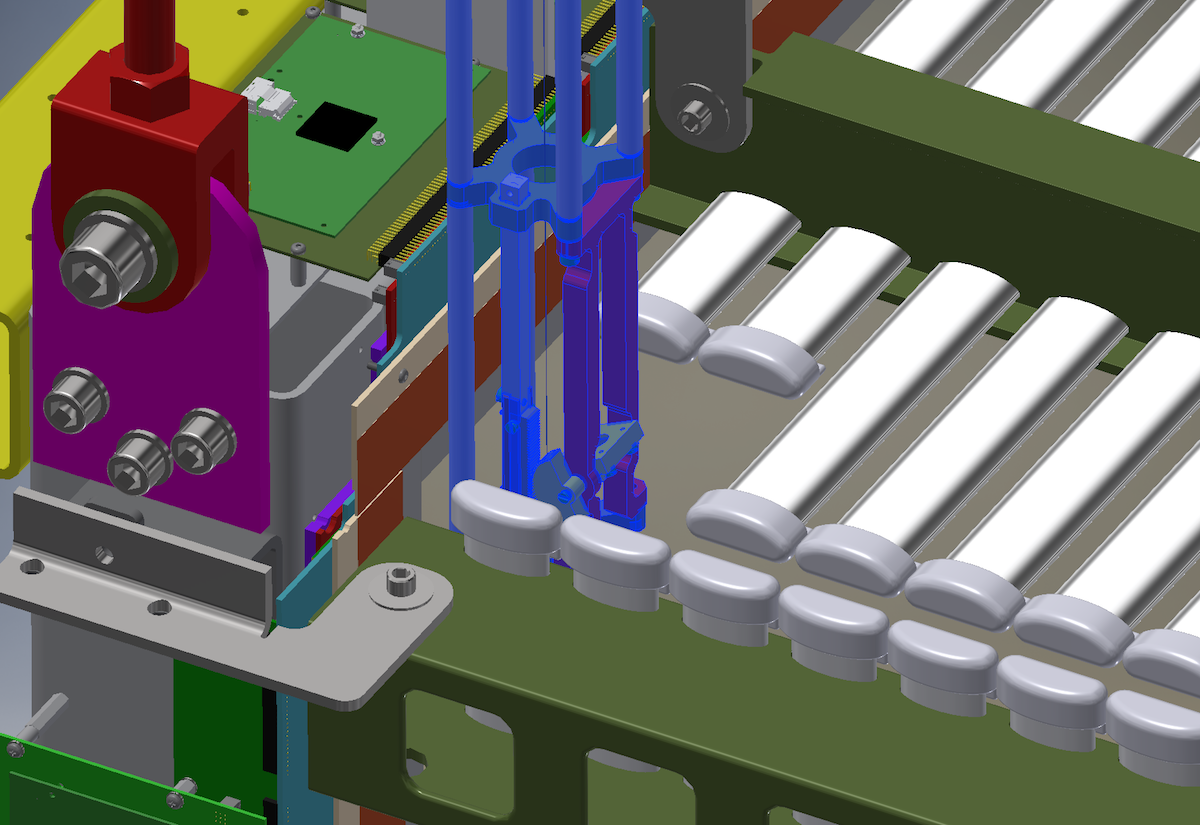
\includegraphics[width=0.7\textwidth]{SBND_Laser_Arrangement.png}
\end{dunefigure}


